% $Id$
%
% Copyright 2011, 2012, 2013, 2014; Daniel Bosk <daniel@bosk.se>
%
% This work is licensed under the Creative Commons Attribution-ShareAlike 3.0 
% Unported license.  To view a copy of this license, visit URL
%
%   http://creativecommons.org/licenses/by-sa/3.0/.
%

%\documentclass[a4paper,titlepage,reqno,final,oneside]{amsbook}
%\documentclass[a4paper,titlepage,reqno,final,twoside]{amsbook}
\documentclass[reqno,twoside,draft]{amsbook}
\usepackage{amsbooka}
\usepackage[utf8]{inputenc}
\usepackage[T1]{fontenc}
\usepackage{xparse}
\usepackage[ibycus,german,english,swedish]{babel}
\usepackage{graphicx}
\usepackage[hyphens]{url}
\usepackage{lettrine}
\usepackage[strict]{csquotes}
\usepackage{setspace}
\usepackage{nomencl}
\usepackage{marginnote}
\usepackage{subfig}
\usepackage{booktabs}
\usepackage[multiple]{footmisc}
\usepackage{verbatim}
\usepackage{asymptote}
\usepackage{hhcount}
\usepackage[binary-units]{siunitx}

\usepackage{ifdraft}
\ifdraft{%
  \usepackage{datetime}
  \usepackage{fancyhdr}
  \usepackage{showlabels}
}{%
  \if@twoside
    \usepackage[a4paper,rmargin=6cm]{geometry}
  \fi
}

\usepackage[natbib,style=alphabetic,maxbibnames=99]{biblatex}
\addbibresource{matematik-1.bib}
%\addbibresource{krypto/introcrypt.bib}
%\addbibresource{pwdanalysis/literature.bib}

\usepackage{interval}
\intervalconfig{soft open fences,scaled}

\usepackage{mleftright}
\usepackage{amssymb}
\usepackage{mathtools}
%\mathtoolsset{showonlyrefs}
\usepackage{amsthm}
\newtheorem{theorem}{Sats}[chapter]
\newtheorem{proposition}{Proposition}[chapter]
\newtheorem{lemma}{Lemma}[chapter]
\newtheorem{corollary}{Korollarium}[chapter]
\newtheorem{conjecture}{Förmodan}[chapter]
\theoremstyle{definition}
\newtheorem{axiom}{Axiom}[chapter]
\newtheorem{definition}{Definition}[chapter]
\newtheorem{example}{Exempel}[chapter]
\newtheorem{exercise}{Övning}[chapter]
\theoremstyle{remark}
\newtheorem{remark}{Anmärkning}[chapter]

\numberwithin{section}{chapter}
\numberwithin{equation}{chapter}
\numberwithin{figure}{chapter}
\numberwithin{table}{chapter}

\usepackage{varioref}
\renewcommand{\reftextbefore}{(föregående sida)}
\renewcommand{\reftextfacebefore}{(föregående sida)}
\renewcommand{\reftextafter}{(nästa sida)}
\renewcommand{\reftextfaceafter}{(nästa sida)}
\renewcommand{\reftextfaraway}[1]{(sidan~\pageref{#1})}
\usepackage{hyperref}
\usepackage[noabbrev,swedish]{cleveref}
\crefname{conjecture}{förmodan}{förmodan}
\crefname{axiom}{axiom}{axiom}
\crefname{exercise}{övning}{övning}
\Crefname{exercise}{Övning}{Övning}
\crefname{corollary}{korollarium}{korollarium}
%\crefname{proposition}{proposition}{proposition}

\renewcommand{\qedsymbol}{Q.E.D.}
\DeclareDocumentCommand{\N}{}{\ensuremath{\mathbb{N}}}
\DeclareDocumentCommand{\Z}{}{\ensuremath{\mathbb{Z}}}
\DeclareDocumentCommand{\Q}{}{\ensuremath{\mathbb{Q}}}
\DeclareDocumentCommand{\R}{}{\ensuremath{\mathbb{R}}}
\DeclareDocumentCommand{\powerset}{}{\ensuremath{\mathcal{P}}}
%\DeclareMathSymbol{\powerset}{\mathord}{MnSyC}{180}
\DeclareDocumentCommand{\U}{}{\ensuremath{\mathcal{U}}}
\DeclareDocumentCommand{\V}{}{\ensuremath{\mathcal{V}}}
\DeclareMathOperator{\card}{card}
\DeclareMathOperator{\tnot}{icke}
\DeclareMathOperator{\tor}{eller}
\DeclareMathOperator{\tand}{och}
\DeclareMathOperator{\congruent}{\equiv}


\makenomenclature{}
\makeindex{}

\includeonly{%
  sannolikhet%
}

\begin{document}
\ifdraft{%
  \fancypagestyle{plain}{%
    \renewcommand{\headrulewidth}{0pt}
    \fancyhead{}
    \fancyfoot[co,ce]{\thepage}
    \fancyfoot[ro,le]{%
      \tt Draft: \today~\currenttime{}
    }
  }
  \fancypagestyle{ams}{%
    \renewcommand{\headrulewidth}{0pt}
    \fancyhead[ce]{\small\leftmark}
    \fancyhead[co]{\small\rightmark}
    \fancyhead[lo,re]{}
    \fancyhead[ro,le]{\thepage}
    \fancyfoot[ro,le]{%
      \tt Draft: \today~\currenttime{}
    }
  }
  \pagestyle{ams}
}{}

\title{%
  Matematik för alla, volym I%
}
\author{%
  Daniel Bosk%
}

\frontmatter
%\begin{abstract}
%    \input{abstract.tex}
%\end{abstract}

\ifdraft{}{%
    \if@twoside
    \newgeometry{rmargin=4cm,lmargin=4cm}
    \fi
}
\maketitle
\ifdraft{}{%
    \if@twoside
    \restoregeometry{}
    \fi
}
%\begin{titlepage}
%   \begin{center}
%       \vskip0.1\textheight
%       \textsc{\huge \...@title}
%       \vskip0.1\textheight
%       \textsc{\large \...@author}
%       \vskip0.7\textheight
%       \textsc{\...@date}
%   \end{center}
%\end{titlepage}

\cleardoublepage{}
{
    \small
    \setlength{\parskip}{0.5em}
    \setlength{\parindent}{0em}
    \vspace*{\fill}
    \input{LICENSE}
}

\tableofcontents
\cleardoublepage{}

%\chapter*{Förord till första utgåvan}
\chapter*{Förord}
\lettrine{D}{agens matematikundervisning} har fått mycket kritik de senaste
åren.
En av de mest framstående kritiseringarna är Skolinspektionens rapport 2010:13,
\emph{Undervisningen i matematik i gymnasieskolan}.
Den så kallade matematiken som de senaste årtiondena dominerat svensk skola
upplevs som räknecentrerad och eleverna lär sig genom memorering snarare än
förståelse.
Detta undervisningsmaterial syftar till att motverka denna typ av undervisning 
och inlärning.
Det ämnar att eleverna ska \emph{förstå} matematik, inte memorera metoder genom
mekaniskt räknande.

Detta verk är utvecklat att behandla det centrala innehållet i ämnesplanen 
Matematik 1c för 2011 års läroplan för gymnasieskolan.
Omfattningen av detta material är en inledning till rigorös matematik, en grund
att bygga fortsatt undervisning på.
Syftet med detta material är således inte att vara ett fördjupningsmaterial,
utan att formalisera matematiken i dagens matematikundervisning.

De gamla kursplanerna och de nya ämnesplanerna för matematik fokuserar båda
mycket på tillämpad matematik.
Det gör även de flesta matematikböcker för skolan.
I dessa framställningar kommer matematiken i sig i skymundan.
Denna text fokuserar mer på \emph{ren matematik}, anledningen är att
matematiken sällan framhålls i sin rena form och svensk tradition är tillämpad
matematik.
Kompendiet är också upplagt annorlunda och ej avsett att följa den
traditionella svenska matematikundervisningen med några givna exempel följt av
ett större antal uppgifter som följer exemplet.
Faktum är att detta kompendium inte innehåller en enda, så kallad,
standarduppgift.
Det innehåller inte några uppgifter över huvud taget, jag har valt att kalla
dem för övningar för att komma bort från detta uppgiftsfokus.
Dessa övningar syftar till att låta läsaren öva sitt matematiska resonerande.
De ska inspirera till reflektion hos läsaren för att hjälpa denne att fördjupa 
sin förståelse för innehållet.

Materialet är framtaget med tanken att ackompanjeras av en undervisande lärare,
tanken är alltså inte att det ska användas för enskild läsning --- även om 
detta naturligtvis är möjligt.
Forskning har visat att lärande som en social process, med diskussioner och
gemensamt resonerande, är bättre för lärande än individuellt arbete.
Tanken är alltså att innehållet ska diskuteras och reflekteras över.
Läsaren uppmuntras därför att läsa materialet och därefter diskutera det med 
någon.

% XXX Extend about the study guide
En studiehandledning för att använda denna text inom gymnasieundervisning finns 
i \cref{Studiehandledning}.

Jag skrev början av detta material som en del av mitt examensarbete på
Civilingenjör- och lärarprogrammet vid Kungliga Tekniska högskolan (KTH) och
Stockholms universitet (SU) under våren 2011.
Jag vill därför rikta ett stort tack till mina handledare
Roy Skjelnes, universitetslektor i matematik vid KTH,
Lil Engström, universitetslektor emerita i matematikdidaktik vid SU, och
till Dan Laksov, professor emeritus i matematik vid KTH,
för värdefulla kommentarer och givande diskussioner under mitt arbete.

Jag har nu vidareutvecklat materialet till att täcka hela ämnesplanen, förfinat 
och utökat vissa delar.
Som lärare anser jag att information och kunskap ska vara fritt tillgängliga 
för alla, det är därför jag tillgängliggör detta verk fritt för alla att ta del 
av.
Jag publicerar det tillsammans med källkoden under licensen Creative Commons 
Erkännande-DelaLika 2.5 Sverige (CC BY-SA 2.5 SE)\footnote{%
  För att se en sammanfattning och kopia av licenstexten besök URL 
  \url{http://creativecommons.org/licenses/by-sa/2.5/se/}.
}.
Detta innebär att vem som helst får bygga vidare på denna text och publicera 
resultatet; de enda krav som föreligger är att resultatet också publiceras 
under denna (eller liknande licens) och att där står att resultatet bygger på 
detta verk.
Därför uppmuntrar jag att bygga vidare på detta arbete, och eventuella 
förbättringar inkorporerar jag mer än gärna tillbaka i detta verk.
Jag lägger även gärna till lektionsförslag eller andra förslag på tillämpningar 
som bilagor i detta verk eller hänvisar till andra tillämpningar som gjorts.

\vspace{2cm}
\begin{flushright}
  \parbox{0.5\textwidth}{%
    Söråker, den 25 juni 2012\\
    \vspace{10pt}%
    Daniel Bosk
  }
\end{flushright}


\mainmatter{}
\ifdraft{%
  \onehalfspacing{}
}{}
% main chapters
% $Id$
%
% Copyright 2011, 2012, 2013, 2014, 2015; Daniel Bosk <daniel@bosk.se>
%
% This work is licensed under the Creative Commons Attribution-ShareAlike 4.0 
% Unported license.  To view a copy of this license, visit URL
%
%   http://creativecommons.org/licenses/by-sa/4.0/.
%
\chapter{Introduktion}\label{Introduktion}
% XXX fysik, kemi använder matematiken
\lettrine{M}{atematiken har funnits} i mer än 5000 år, men började utvecklas i 
riktning mot dagens matematik först omkring 300 f.v.t.\ i antikens Grekland 
\cite{Kline1990mtf1}.
Innan dess var matematiken endast räkning, ett verktyg för att beräkna skatter 
och konstruera byggnadsverk.

Ordet matematik har enligt~\cite{OED2013maths} sitt ursprung i grekiskans 
\emph{\ibygr{ma'qhma} (m{\'a}th{\=e}ma)}, vilket betyder \emph{lärande, 
studier, vetenskap}.
Det är i det antika Grekland som dagens matematik har sitt ursprung.
De studerade främst geometri och gjorde detta genom att sätta upp några 
grundläggande antaganden, kallade postulat eller axiom, som de var övertygade 
om att de stämde överens med verkligheten.
Dessa var enkla antaganden, såsom att två parallella linjer aldrig kommer att 
skära varandra.
Utifrån dessa enkla postulat härledde de olika geometriska resultat med hjälp 
av logik och de kunde bevisa att det måste vara på ett visst sätt.
Även om de kunde se genom några enkla experiment hur saker förhöll sig till 
varandra nöjde de sig inte utan ett bevis utifrån postulaten eller tidigare 
bevisade resultat.
Anledningen till detta är enkel: för att övertyga sig om att någonting alltid 
stämmer, då räcker det inte med att testa tre fall, det räcker inte med 
hundratals fall, inte en tusentals --- dessa fall kanske avviker, eller att 
inget av dem är det specialfall som avviker.

Detta har inspirerat matematiker genom historien och är den drivkraft som 
verkat för att matematiken utvecklats till det som den är idag.
Dagens matematik bygger likt grekernas på några enkla grundantaganden som vi 
kallar för axiom.
Vidare måste begrepp som vi använder definieras tydligt för att vi exakt ska 
veta vad som menas med dem.
Detta var drivkraften bakom axiomatiseringen av de naturliga talen som vi 
kommer att se i \cref{DeNaturligaTalen}, bakom grundläggningen av de hela 
talen i \cref{ch:Heltalen}, de rationella talen i 
\cref{ch:Rationella} och de reella talen i \cref{ch:Reella}.
Länge hade matematikerna tagit talen som självklara, men vid 1800-talets mitt 
behövde de veta tydligare vad ett tal var för att kunna gå vidare.
Det som är intressant är att behovet av en axiomatisering uppstod historiskt i 
omvänd ordning av hur de logiskt är uppbyggda och presenteras i denna text.
För en detaljerad redogörelse över den historiska utvecklingen hänvisas till 
\citet{Kline1990mtf3}.

I en definition av ett objekt eller egenskap sätter vi upp regler för hur ett 
objekt som är av denna typ eller har denna egenskap ska bete sig.
Om vi kan visa att ett objekt uppfyller reglerna i definitionen, då måste
objektet också vara av den typen eller ha den egenskapen.

\begin{example}\label{ex:cykel}
  Vi använder följande definition: en \emph{cykel} har åtminstone ett hjul och 
  vevarmar med pedaler som används för att driva hjulen och ge cykeln fart.

  Om vi tittar på fordonet i \cref{fig:cykel} ser vi att det har 
  åtminstone ett hjul (det har två), det har vevaxlar med pedaler som används 
  för att driva hjulen och således ge fordonet fart.
  Alltså måste det enligt vår definition vara en cykel.
\end{example}
\begin{figure}
  % XXX create figs/cykel.eps
  \includegraphics[width=0.7\textwidth]{figs/cykel.eps}
  \caption{En illustration av en cykel.}\label{fig:cykel}
\end{figure}

\begin{example}\label{ex:bil}
  Vi använder samma definition som i \cref{ex:cykel}.
  Om vi tittat på fordonet i figur \cref{fig:sparkcykel} ser vi att det 
  har åtminstone ett hjul.
  Det saknas dock vevarmar för att driva hjulen.
  Vi kan således konstatera att en sparkcykel enligt definitionen i 
  \cref{ex:cykel} inte är en cykel.
\end{example}
\begin{figure}
  % XXX create figs/sparkcykel.eps
  \includegraphics[width=0.7\textwidth]{figs/sparkcykel.eps}
  \caption{En illustration av en sparkcykel.}\label{fig:sparkcykel}
\end{figure}

Med denna typ av definitioner kan vi veta exakt, vi kan bevisa att ett objekt 
är av en specifik typ --- likt vi gjorde i exemplen ovan.
Vi kan också göra det omvända, om ett objekt är av denna typen uppfyller det de
givna reglerna.
Exempelvis, om någon säger att de har en cykel, då måste den ha åtminstone ett 
hjul och vevarmar med pedaler som driver den framåt.
När vi bevisar saker kan vi alltså utgå från enbart dessa regler, det är detta 
som är grunden inom matematiken.


%%%%%%%%%%%%%%%%%%%%%%%%%%%%%%%%%%
% NOTATION
%%%%%%%%%%%%%%%%%%%%%%%%%%%%%%%%%%
\section{Den missförstådda algebran}

Innan vi går vidare till våra studier av matematiken ska vi ägna några rader åt 
något som i onödan förrvirrat alltför många: algebra.
Algebran har många gånger beskrivits som \enquote{att räkna med bokstäver}, 
vilket är tämligen missvisande, vi ska i detta avsnitt förklara vad algebra 
faktiskt är.

I vårt dagliga tal har vi diverse språkliga konstruktioner för att veta vilka 
objekt vi samtalar om, exempelvis \enquote{den svarta bilen närmast hitåt} 
eller \enquote{korsningen närmast skolan}.
Vi använder dessa beskrivningar utan större ansträngning.
Ibland blir det dock fel, vi har säkert alla hamnat i en situation som krävt 
uttrycket \enquote{jaha, du menar den, jag trodde att du menade något helt 
annat}.
Då måste vi förbättra noggrannheten i våra beskrivningar av objekten för att 
bli förstådda utan vidare missförstånd.

Vi kan också prata om klasser av objekt, exempelvis träd.
De flesta har säkert stött på uttrycken \enquote{en björk har löv} eller 
\enquote{björkar har löv}, \enquote{en tall har barr} eller \enquote{tallar har 
barr}.
Det är för de flesta självklart vad som menas med en björk, att det är ett träd 
av släktet björk (\emph{betula}).
Den specifika arten spelar ingen roll, exempelvis hängbjörk (\emph{betula 
pendula}) och dvärgbjörk (\emph{betula nana}) är båda björkar.
Uttryckssättet brukar användas i meningar som \enquote{en björk har vit-svart 
stam} eller \enquote{björkar har vit-svarta stammar}.

\begin{exercise}
  Prata med någon om valfritt ämne, var uppmärksam på hur ni uttrycker er för 
  att säkerställa att ni \enquote{pratar om samma sak}.
\end{exercise}

Matematiken är inte särskilt mycket konstigare än vanligt språk.
Ett av matematikens främsta verktyg är just språket, utan det skulle vi inte 
kunna uttrycka våra tankar på ett effektivt sätt.
Ett annat ovärderligt verktyg är pennan med tillhörande papper.
Detta hjälper oss dels att spara våra tankar, men framförallt att strukturera 
dem.

Säg nu att vi vill diskutera olika exotiska blommor som finns hos en 
blomsterhandlare.
Då vi själva inte är experter på exotiska blommor vet vi inte namnet på dem, så 
vi kan inte använda namnen för att diskutera dem.
Ibland kanske vi släktets namn, exempelvis orkidé (\emph{orchidaceae}), men det 
finns så många olika orkidéer att detta inte alltid hjälper.
Om alla blommor är av olika färg skulle vi kunna använda färgen för att 
identifiera de olika blommorna, exempelvis \enquote{jag tycker bäst om den 
gröna blomman}.
Men, det är sällan detta är fallet, så det är inte en hållbar metod.
En annan naturlig metod är att numrera dem, exempelvis \enquote{jag tycker bäst 
om den första blomman vi tittade på}.
Denna metod är mer hållbar.

Nu vill vi göra samma sak med papper och penna, kanske för att göra en 
inköpslista.
Då det tar mycket längre tid att skriva något än att säga samma sak, vill vi 
naturligtvis ha en kortare notation.
Vi kanske bara skriver \enquote{1:a} eller bara \enquote{1}, istället för 
\enquote{den första blomman} eller \enquote{blomma nummer ett}.
Om vi nu vill ha flera av en sort, då finns det en risk att vi förvirrar oss om 
vi skriver \enquote{2 3}.
Betyder detta att vi vill ha två av den tredje blomman eller tre av den andra 
blomman?
En bättre lösning är därför att vi hittar på namn eller symboler till de olika 
blommorna.
Vi skulle kunna rita en liten bild av de blommor vi tycker bäst om och vill 
köpa.
Detta tar dock tid, och blir inte alltid särskilt bra.
Vi kan därför använda symboler som vi redan har namn på, och som vi kan skriva 
väldigt effektivt: vårt alfabet.
Låt den första blomman vara \(a\), den andra \(b\), och så vidare.
Då finns det ingen risk att vi blandar ihop antalet med sorten likt ovan, vi 
kan skriva exempelvis \(2c\) och vet exakt vad vi menar.

Detta är bakgrunden till den matematiska notationen med bokstäver.
Det är således inget märkligt med den matematiska notationen som skrämt så 
många, det är helt enkelt ett enkelt sätt att namnge saker på ett skrivvänligt 
sätt.
En nackdel är att det finns så få bokstäver.
Därför brukar man ibland även ta till det grekiska alfabetet för att få fler 
bokstäver.
En sammanfattning av detta finns i \cref{tbl:greekalpha}.

\begin{table}
  \caption{Det grekiska alfabetet.}
  \begin{tabular}{lll}
    \textbf{Versal} & \textbf{Gemen} & \textbf{Uttal} \\
    \toprule
    \(A\) & \(\alpha\) & alfa \\
    \(B\) & \(\beta\) & beta \\
    \(\Gamma\) & \(\gamma\) & gamma \\
    \(\Delta\) & \(\delta\) & delta \\
    \(E\) & \(\epsilon\) & epsilon \\
    \(Z\) & \(\zeta\) & zeta \\
    \(H\) & \(\eta\) & eta \\
    \(\Theta\) & \(\theta\) & theta \\
    \(I\) & \(\iota\) & iota \\
    \(K\) & \(\kappa\) & kappa \\
    \(\Lambda\) & \(\lambda\) & lambda \\
    \(M\) & \(\mu\) & my \\
    \bottomrule
  \end{tabular}
  \hspace{1em}
  \begin{tabular}{lll}
    \textbf{Versal} & \textbf{Gemen} & \textbf{Uttal} \\
    \toprule
    \(N\) & \(\nu\) & ny \\
    \(\Xi\) & \(\xi\) & xi \\
    \(O\) & \(o\) & omikron \\
    \(\Pi\) & \(\pi\) & pi \\
    \(P\) & \(\rho\) & rho \\
    \(\Sigma\) & \(\sigma\) & sigma \\
    \(T\) & \(\tau\) & tau \\
    \(Y\) & \(\upsilon\) & ypsilon \\
    \(\Phi\) & \(\phi\) & phi \\
    \(X\) & \(\chi\) & khi \\
    \(\Psi\) & \(\psi\) & psi \\
    \(\Omega\) & \(\omega\) & omega \\
    \bottomrule
  \end{tabular}\label{tbl:greekalpha}
\end{table}

Oftast brukar bokstäverna väljas så att de underlättar för minnet, exempelvis 
\(b\) för blomma och \(k\) för kruka.
Sedan kan man använda subskript, exempelvis kan vi beteckna de olika blommorna 
ovan som \(b_1, b_2\) och så vidare.
Då kan vi skilja blommorna från krukorna, som vi kan benämna \(k_1, k_2\) och 
så vidare.


%%%%%%%%%%%%%%%%%%%%%%%%%%%%%%%%%%%%%
% VAD ÄR MATEMATIK?
%%%%%%%%%%%%%%%%%%%%%%%%%%%%%%%%%%%%%
\section{Vad är matematik?}
% - Skillnaden mellan matematiken och andra vetenskaper.
% - Abstrakt konstruktion som endast finns i sinnet.
% - Naturvetenskap i Sverige, filosofi i resten av världen.
%   - Sveriges störta bidrag till matematikhistorien är att vi tog död på René
%     Descartes (Touraine, 1596--Stockholm, 1650).
% - Behöver inte ha någon till synes uppenbar tillämpning, det är vackert.
%   - Pierre de Fermat (160{1,7,8}--1665), advokat, upphovsman till Fermats
%     lilla sats och Fermats stora (sista) sats.
%   - Fermat--Euler satsen är grunden för kryptosystemet när man loggar in på
%     banken via internet.
% - Demokratiskt organiserad. Alla kan bidra, ex. Fermat var advokat.
Som antyddes ovan, kan matematiken beskrivas som studiet av abstrakta 
konstruktioner.
Med abstrakta konstruktioner menar vi saker som endast finns i våra tankar, 
eller vad Platon (cirka 428--348 f.v.t.) kallade \enquote{idévärlden}.
Vi sätter upp axiomen och definitionerna, vilka vi skulle kunna kalla våra 
spelregler, och undersöker sedan vad dessa spelregler ger upphov till.

Historiskt har matematiken ofta varit sammankopplad med studiet av
verkligheten.
Vi har kunnat studera verkligheten med hjälp av matematiken genom att våra
grundregler varit grundläggande principer för verkligheten\footnote{%
  Se exempelvis Euklides postulat för geometrin i \cref{ch:Geometri} eller~\cite[kap.\ 4]{Kline1990mtf1}.
}.
Men trots detta är matematiken skild från verkligheten.
De axiom vi utgår ifrån behöver inte vara principer från verkligheten.
Det finns matematiska konstruktioner som kan te sig så verklighetsfrånkopplade
att icke-matematiker ifrågasätter varför de studeras, och detta för oss in på
ett viktigt konstaterande:
Matematiken har inte alltid studerats enbart för att kunna dra slutsatser om
verkligheten.
Många matematiker genom historien studerade matematiken enbart för den rena
matematikens skull --- för att den var vacker, inte för att den gick att
tillämpa på verkligheten.
De ville utforska den värld som spänns upp av axiomen.
Exempel på sådana är Pierre de Fermat (cirka 1607--1650) som är upphovsman till 
den kända \emph{Fermats stora sats}.
Han var advokat och amatörmatematiker.
Fermats stora sats eller \emph{Fermats sista sats} säger att ekvationen
\(x^n+y^n=z^n\), där \(x,y\) och \(z\) är heltal, saknar lösningar för heltal
\(n\) som är större än två.
Fermat lämnade en anteckning i marginalen av sin kopia av Diophantus (omkring 
år 250) bok \emph{Arithmetica} att han hade ett bevis för detta, men att 
marginalen var för liten för att rymma det.
Det tog matematiker ända fram till år 1994 att bevisa satsen, så möjligen
hade Fermat inte ett korrekt bevis då beviset som togs fram inryms på tusentals 
sidor och krävde hundratals år av matematisk utveckling.
Han hade däremot ett korrekt bevis för sin \emph{lilla sats} som säger att om
\(p\) är ett primtal, då ger \(a^{p-1}\) alltid resten \(1\) vid division med
\(p\).
(Detta tas upp i \cref{ch:Talteori}.)
Leonard Euler (1707--1783) generaliserade Fermats lilla sats till att gälla även
sammansatta tal, och denna generalisering är känd som \emph{Eulers sats} eller 
ibland \emph{Fermat--Eulers sats}.
Resultaten för dessa hade inget tillämpningsvärde för tiden, utan drivkraften
var att utforska matematikens vackra värld och finna vackra resultat som dessa.
År 1978 publicerades dock en tillämpning av satsen.
Det var Ronald Rivest (1947--), Adi Shamir (1952--) och Leonard Adleman 
(1945--) som då publicerade ett kryptosystem sedermera känt som RSA\@.
RSA-systemet bygger på Eulers sats och systemet ligger till grund för
mycket av den säkra kommunikationen som sker på internet idag.
Det dröjde alltså cirka 300 år innan någon fann en tillämpning, innan dess var 
det vara ett vackert resultat.

Detta visar även vikten av den så kallade grundforskningen, den forskning som 
inte har någon omedelbar tillämplighet, utan enbart syftar till att fördjupa 
mänsklighetens kunskap inom området.
Detta är inte viktigt bara för matematiken utan för alla vetenskaper.
För vi kan ställa oss frågan: hade vi hade haft säker kommunikation på internet
idag om vi bara utforskat det som verkat direkt tillämpbart?

%Vi ska med det gå vidare till nästa kapitel som handlar om matematikens grund
%-- logik och bevis.
%Det är logiken som är matematikens verktyg för att resonera kring de axiom som
%vi antagit.


%%%%%%%%%%%%%%%%%%%%%%%%%%%%%%%%%
% UPPLÄGG
%%%%%%%%%%%%%%%%%%%%%%%%%%%%%%%%%
%\section{Bokens upplägg}
%...
%

\ifdraft{}{%
  \part{Den matematiska grunden}
}
\chapter{Logik och bevis}
\label{ch:Logik}
\lettrine{M}{atematiken har sin} grund i logiken.
Det är logiken som ger matematiken möjligheten till ett resonemang och
möjligheten till härledning.
Matematiken utgår från några få grundläggande antaganden, kallade \emph{axiom},
från vilka matematiska resultat härleds.
En matematiker nöjer sig således inte med att undersöka några exempel -- eller
göra experiment -- inte ens tusen- eller miljontals exempel duger.
Det är detta som skiljer matematiken från exempelvis fysiken och kemin, trots
att dessa till mycket stor omfattning använder matematiken som hjälpmedel.
Vi känner inte till alla grundläggande principer för fysiken och kemin, utan 
det är (återstoden av) dessa vi försöker att finna genom grundforskningen inom 
dessa ämnen.
Vi känner däremot till alla grundläggande principer för matematiken, detta för
att matematiken är skapad av oss -- det är vi som bestämt dessa principer.
I detta kapitel ska vi lära oss mer om dessa.


%%%%%%%%%%%%%%%%%%%%%%%%%%%%%%%%%%
% LOGIK
%%%%%%%%%%%%%%%%%%%%%%%%%%%%%%%%%%
\section{Logik}

All matematisk argumentation består av \emph{utsagor}.
Utsagor\index{utsaga} är deklarativa meningar som kan klassificeras som 
antingen \emph{sanna} eller \emph{falska}.
Vi behöver inte alltid veta precis vilket, men det måste vara den ena eller den
andra -- aldrig båda.
Detta kallas inom logiken för \emph{lagen om det uteslutna tredje}\index{lagen 
om det uteslutna tredje}.
Om vi tittar på följande meningar:
\begin{enumerate}
  \item Denna text är skriven på svenska.
  \item Grön är en fin färg.
  \item Denna mening är falsk.
  \item Det finns oändligt många primtalstvillingar.
  \item \(x^2+1=0\)
\end{enumerate}

Den första meningen är en utsaga, och den är sann.
Den andra är ej en utsaga i logisk bemärkelse, det är en smaksak.
Den tredje meningen är ej en utsaga, den kan varken vara sann eller falsk
eftersom att det leder till motsägelsefulla slutsatser.
Den fjärde meningen är en utsaga, ingen vet dock om den är sann eller falsk.
Den femte och sista symbolföljden är en utsaga, men vi vet inte vad \(x\) är så
vi kan inte uttala oss om den skulle vara sann eller falsk.
Detta visar vikten av att tydligt specificera alla delar av en utsaga, så att
det är alldeles klart vad vi menar.
Den femte utsagan skulle behöva ändras till exempelvis \enquote{det finns ett
komplext tal \(x\) sådant att \(x^2+1=0\)} för att den skulle vara sann.
Om vi istället ändrat den till \enquote{det finns ett heltal \(x\) sådant att
\(x^2+1=0\)} skulle den vara falsk oavsett hur vi väljer \(x\) eftersom att
det inte finns ett sådant heltal.  En utsaga som alltid är falsk kallar vi för 
\emph{motsägelse}\index{motsägelse!utsaga} eller
\emph{kontradiktion}\index{kontradiktion|see {motsägelse}}.
En utsaga som alltid är sann kallar vi för \emph{tautologi}\index{tautologi}.

Två utsagor \(P\) och \(Q\) sägs vara logiskt 
ekvivalenta\index{ekvivalens!logisk} om \(P\) är sann
precis när \(Q\) är sann och följaktligen om \(P\) är falsk precis när \(Q\)
är falsk.
Vi skriver detta som \(P\equiv Q\).

\subsection{Kombinerade utsagor}

Vi vill också kunna forma nya utsagor från redan kända, detta genom att
kombinera och modifiera dem.
Om \(P\) är en utsaga, då säger vi att \emph{negationen}\index{negation!logisk} 
av \(P\), betecknad \(\lnot P\) eller \(\tnot P\), är falsk precis när \(P\) är 
sann och sann precis när \(P\) är falsk.
Vi kommer då fram till \emph{lagen om dubbelnegation}\index{lagen om 
dubbelnegation}.
Om vi funderar på vad som händer om vi tar \(\lnot(\lnot P)\) så kommer vi
fram till att \(P\equiv \lnot(\lnot P)\).
\begin{example}
  Ett exempel på negation, låt \(P\) vara utsagan \enquote{vi befinner oss i
  Sverige}.
  Då blir \(\lnot P\) \enquote{vi befinner oss inte i Sverige}.
  Vi kan också se att \(\lnot(\lnot P)\) blir \enquote{att vi inte befinner oss 
  inte i Sverige}, vilket är lite svårare att läsa men resulterar i att vi 
  måste befinna oss i Sverige.
\end{example}
\begin{example}
  Vi kan också titta på följande utsaga, \enquote{alla svenskar tycker om
  surströmming}.
  Negationen av den utsagan är \emph{inte} att ingen svensk tycker om
  surströmming, utan den är \enquote{inte alla svenskar tycker om 
  surströmming}.
  Det räcker då med att det finns en svensk som inte tycker om
  surströmming -- detta är en viktig skillnad att inte ta fel på!
\end{example}

Vi kan också kombinera utsagor genom \emph{konjunktioner}\index{konjunktion}.
Om \(P\) och \(Q\) är utsagor, då betecknar vi konjunktionen som \(P\tand Q\)
eller \(P\land Q\).
Konjunktionen är sann då både \(P\) och \(Q\) båda är sanna och falsk annars.
\begin{example}\label{ex:KonjunktionInternet}
  Låt \(P\) vara utsagan \enquote{jag bor i Sverige} och \(Q\) vara utsagan 
  \enquote{jag har en internetuppkoppling}.
  Då kan vi skapa den nya utsagan \(P\land Q\) som blir \enquote{jag bor 
    i Sverige \emph{och} jag har en internetuppkoppling}.
\end{example}

\begin{exercise}
  När är de olika utsagorna \(P\), \(Q\) och \(P\land Q\) i
  \cref{ex:KonjunktionInternet} sanna respektive falska?
\end{exercise}

Vi har också \emph{disjunktionen}\index{disjunktion} som betecknas \(P\tor Q\) 
eller \(P\lor Q\).
Disjunktionen är sann om antingen \(P\) eller \(Q\) eller båda är sanna, och är
således falsk endast när \(P\) och \(Q\) båda är falska.
\begin{example}
  Julfika kräver lussebullar \emph{eller} julfika kräver pepparkakor.
  Denna utsaga säger att om vi fikar lussebullar, då är det julfika.
  Den säger också att det är julfika om vi fikar pepparkakor.
  Den säger också att det är julfika om vi fikar både lussebullar och 
  pepparkakor samtidigt.
\end{example}

Konjunktionen och disjunktionen sammanfattas i en sanningstabell i
\cref{tbl:SanningKonjunktionDisjunktion}.

\begin{table}
  \caption{%
    Sanningstabell för konjunktionen och disjunktionen.
    S betecknar sant och F betecknar falskt.
  }
  \begin{tabular}{cccc}
    \(P\)  & \(Q\)   & \(P\land Q\)  & \(P\lor Q\) \\
    \toprule
    S      &  S      & S             & S \\
    S      &  F      & F             & S \\
    F      &  S      & F             & S \\
    F      &  F      & F             & F \\
    \bottomrule
  \end{tabular}\label{tbl:SanningKonjunktionDisjunktion}
\end{table}

\begin{exercise}\label{xrc:tartkalas}
  Vilken av följande logiska utsagor passar bäst för ett tårtkalas?
  På ett kalas
  \begin{enumerate}
    \item äts tårta \emph{och} dricks saft \emph{och} äts kakor
      \emph{och} dricks kaffe \emph{och} dricks te.
    \item äts tårta \emph{eller} dricks saft \emph{eller} äts kakor
      \emph{eller} dricks kaffe \emph{eller} dricks te.
  \end{enumerate}
\end{exercise}

\begin{exercise}
  Ingen av utsagorna i \cref{xrc:tartkalas} är egentligen riktigt bra 
  utsagor för att avgöra om något är ett tårtkalas.
  \begin{enumerate}
    \item Diskutera bristerna i de olika utsagorna.
    \item Utforma en egen bättre utsaga.
  \end{enumerate}
\end{exercise}

Hittills har vi kombinerat konjunktioner med konjunktioner och disjunktioner 
med disjunktioner, men det går naturligtvis även att kombinera konjunktioner 
med disjunktioner.
Vi visar här ett exempel på detta.

\begin{example}\label{ex:aldersgrans}
  I Sverige är åldersgränserna för film följande: under 7 år, under 11 år och 
  under 15 år~\cite{aldersgranser}.
  En film som inte får ses av barn under 11 år får ses av barn som uppfyller 
  följande utsaga: barnet är minst 11 år \emph{eller} barnet är minst 7 år 
  \emph{och} i vuxens sällskap.
  Notera att vi här kombinerat tre utsagor, först med disjunktion och sedan med 
  konjunktion.
\end{example}

\begin{exercise}
  Du kanske märkte av ett problem med utsagan i \cref{ex:aldersgrans}, om 
  inte kommer du att uppmärksamma det nu.
  Utsagan i exemplet har följande form: \(P\lor Q\land R\).
  Undersök om det spelar någon roll om vi tar \(P\lor Q\) eller \(Q\land R\) 
  först, det vill säga om \(P\lor (Q\land R)\equiv (P\lor Q)\land R\).
\end{exercise}

\begin{exercise}
  Testa att kombinera negationer, konjunktioner och disjunktioner, går det
  att forma några logiskt ekvivalenta utsagor?
\end{exercise}

\subsection{Implikationer}

Implikation är synonymt med ordet 
\emph{medför}\index{implikation}\index{medför|see {implikation}}.
Om \(P\) och \(Q\) är utsagor säger vi att \(P\) \emph{implicerar} \(Q\) eller
\emph{om \(P\), då \(Q\)}.
Vi ska undersöka när denna sammansatta utsaga bör vara sann och när den bör
vara falsk.
Låt oss formulera ett exempel.
\begin{example}
  Låt \(P\) vara utsagan \enquote{jag vinner pengar} och \(Q\) vara utsagan
  \enquote{jag köper nya böcker till skolan}.
  Utsagan \(P\implies Q\) blir då \enquote{\emph{om} jag vinner pengar,
  \emph{då} köper jag nya böcker till skolan}.
\end{example}
Implikationen är uppenbart falsk om jag vinner pengar men inte köper böcker till
skolan, men sann om jag köper böcker.
Annars, om jag inte vinner pengar, då har jag heller inte lovat att köpa
böcker till skolan.
Då måste utsagan vara sann i det fallet.
Men att jag inte vinner pengar hindrar mig ju inte att köpa böcker till
skolan ändå, följaktligen borde utsagan vara sann även i det fallet.
Det är detta resonemang som gjort att sanningsvärdena för implikationen är 
valda som de är.
Implikationens olika sanningsvärden sammanfattas i den vänstra delen av 
\cref{tbl:SanningImplikation}.

Vi kan naturligtvis vända på implikationen, om \(P\) och \(Q\) är utsagor och
\(P\implies Q\) då säger vi att dess \emph{invers}\index{invers!logisk} är 
\(Q\implies P\).
Inversen för en implikation är inte nödvändigtvis logiskt ekvivalent med
implikationen.
Ett exempel får illustrera.
\begin{example}\label{ex:kontrapositiv}
  Låt \(P\) vara utsagan \enquote{vi är i Stockholm} och \(Q\) vara utsagan 
  \enquote{vi är i Sverige}.
  Då blir \(P\implies Q\) utsagan \enquote{om vi är i Stockholm, då är vi i
  Sverige}.
  Dess invers \(Q\implies P\), \enquote{om vi är i Sverige, då är vi i
  Stockholm}, är däremot inte sann eftersom att vi skulle kunna vara i
  exempelvis Sundsvall, Göteborg eller Kiruna som också är städer i Sverige.

  Om vi däremot tittar på utsagan \(\lnot Q\implies \lnot P\), det vill säga
  \enquote{om inte vi är i Sverige, då är vi inte i Stockholm}, ser vi att 
  denna måste vara sann samtidigt som \(P\implies Q\).
\end{example}
Den senare utsagan i \cref{ex:kontrapositiv}, \(\lnot Q\implies \lnot P\), 
kallas för den \emph{kontrapositiva}\index{kontrapositiv!utsaga} utsagan av 
\(P\implies Q\).

Om \(P\implies Q\) och \(Q\implies P\) båda skulle vara sanna, vilket ibland är 
fallet, då skriver vi detta som \(P\iff Q\).
Utsagan \(P\iff Q\) kallas för 
\emph{dubbelimplikation}\index{dubbelimplikation|see {logisk ekvivalens}} eller
\emph{ekvivalens}\index{ekvivalens!logisk} och är sann då \(P\) och \(Q\) båda 
är sanna och då de båda är falska.
Den utläses som \emph{\(P\) om och endast om \(Q\)}\index{om och endast om|see 
{logisk ekvivalens}}.
\enquote{Om och endast om} förkortas ibland som \enquote{omm}.
Vi kan se att \(\iff\) får samma betydelse som \(\equiv\).

\begin{exercise}
  Undersök några olika logiska utsagor, likt den kontrapositiva utsagan, och se 
  om du kan finns några intressanta ekvivalenser.
\end{exercise}

Vi ska nu avsluta med en viktig logisk ekvivalens till implikationen.
Denna ligger till grund för motsägelsebevis.
Utsagan \((P\land\lnot Q)\implies C\), där \(C\) är en motsägelse och
därmed alltid är falsk, är logiskt ekvivalent med \(P\implies Q\).
Detta ses tydligast i en sanningstabell, och den är given i
\cref{tbl:SanningImplikation} tillsammans med implikationen och dess
kontrapositiva utsaga.
Implikationen \(P\implies Q\) är bara falsk när \(P\) är sann och \(Q\) är
falsk.
Konjunktionen \(P\land\lnot Q\) är sann endast när \(P\) är sann och \(Q\) är
falsk.
Om \(C\) alltid är falsk, då kommer \(P\land\lnot Q\implies C\) att vara falsk
endast när \(P\land\lnot Q\) är sann.
Men det är ju precis när \(P\) är sann och \(Q\) är falsk, det vill säga när
\(P\implies Q\) är falsk.
Följaktligen måste de vara logiskt ekvivalenta.

\begin{table}
  \caption{%
    Sanningstabell för implikationen och dess logiskt ekvivalenta former.
    S betecknar sant och F betecknar falskt.
  }
  \begin{tabular}{ccccccc}
    \(P\) &
    \(Q\) &
    \(P\implies Q\) &
    \(\lnot(P\land \lnot Q)\) &
    \(\lnot Q\implies \lnot P\) &
    \(C\) & \((P\land\lnot Q)\implies C\) \\
    \toprule
    S & S & S & S & S & F & S \\
    S & F & F & F & F & F & F \\
    F & S & S & S & S & F & S \\
    F & F & S & S & S & F & S \\
    \bottomrule
  \end{tabular}\label{tbl:SanningImplikation}
\end{table}


%%%%%%%%%%%%%%%%%%%%%%%%%%%%%%%%%%
% AXIOM, SATSER OCH BEVIS
%%%%%%%%%%%%%%%%%%%%%%%%%%%%%%%%%%
\section{Axiom, satser och bevis}

För att det ska kunna gå att härleda någonting måste det finnas
några grundläggande utsagor som en grund att bygga på.
Dessa utsagor kallar vi för \emph{axiom}\index{axiom}, och det är från dessa
alla matematiska härledningar utgår.
Vi har också definitioner som indirekt kan specificera axiom.

Vi har ovan redan sett några axiom, nämligen de logiska axiomen.
Det vill säga sanningstabellerna vi tittat på ovan, de fungerar som axiom för 
logiken.
Vi var dock inte tydliga med att dessa var axiom eftersom att vi inte visste 
vad ett axiom var då.
Vi ska i kommande kapitel ta upp de matematiska axiomen.
Det finns axiom som används i nästan all matematik, dessa är axiomen för
mängdläran (\cref{ch:Mangder}), och det finns olika axiomuppsättningar 
inom specifika områden inom matematiken.
Exempelvis ska vi se en axiomuppsättning för geometri 
i \cref{ch:Geometri}, denna gäller för klassisk geometri, det vill säga 
geometri i plana ytor.
I sfärisk geometri, geometri på ytan av en rund boll, som vi inte tar upp 
i denna volym, byts några av axiomen ut.

Grunden må vara viktig att stå på, men möjligheten att ta oss vidare till nya 
resultat -- satser -- är också av yttersta vikt.
Faktum är ju att vi tidigare behövde logiken för att kunna resonera och dra
slutsatser, för att kunna bevisa nya resultat.
Nya resultat, som är implikationer eller dubbelimplikationer, sammanfattas i
något som kallas för \emph{satser}\index{sats}.
En sats ges oftast på formen \enquote{om dessa villkor \(P\) är uppfyllda, då 
gäller även \(Q\)}, där \(P\) och \(Q\) är utsagor.
Men en sats kan inte bara presenteras utan vidare, den kräver alltid ett
\emph{bevis}\index{bevis}.
Ett bevis är en logisk härledning som utgår från axiomen och andra tidigare
bevisade satser för att visa att om \(P\) är sann då måste även \(Q\) vara sann
precis då.
Det vill säga visa att implikationen är sann.

Satsen är huvudbegreppet, men vi har även andra typer av satser.
Vi har \emph{lemman}\index{lemma}, som är hjälpsatser\index{hjälpsats}.
De är också satser, men av mindre betydelse.
Dessa behöver vi för att visa ett mindre resultat för att beviset för en annan
sats inte ska bli onödigt långt.
Vi har även \emph{korollarier}\index{korollarium}, som är
följdsatser\index{följdsats}.
Detta är satser som följer mer eller mindre direkt från en annan sats och har
därför ett mycket kort bevis.

Vi ska nu titta på några vanliga bevismetoder.
När ett bevis genomförs och presenteras brukar detta avslutas med 
\textsc{Q.E.D.}, som är en förkortning för latinets \emph{Quod Erat
Demonstrandum} och betyder \enquote{vilket skulle visas}.
Detta är ett arv från tiden då latin var det vetenskapliga språket och mer
eller mindre all vetenskaplig kommunikation skedde på latin.
Det skulle kunna jämföras med engelskans position idag.

Vi kommer nedan att beskriva den bakomliggande idén för respektive bevismetod.
Därefter kommer vi att se dem tillämpas i resterande kapitel i boken.

\subsection{Motexempelbevis}

Vi börjar med den enklaste bevismetoden.
Om någon skulle påstå att \enquote{alla svenskar tycker om surströmming}, då 
räcker det med att vi hittar en svensk som inte tycker om surströmming för att
motbevisa påståendet.
Det vill säga, vi hittar ett motexempel\index{motexempelbevis}.
Kom ihåg från tidigare att negationen av utsagan \enquote{alla svenskar tycker 
om surströmming} är \enquote{det finns åtminstone en svensk som inte tycker om
surströmming} och att det är denna utsaga som vi bevisar genom att finna en
sådan svensk.

\subsection{Direkta bevis}

Vi låter \(P\) och \(Q\) vara utsagor.
För att \emph{hypotesen}\index{hypotes} \(P\) ska implicera 
\emph{konklusionen}\index{konklusion} \(Q\) måste \(P\) vara sann
precis när \(Q\) är sann.
Vi åstadkommer detta genom konstruktionen av en kedja av implikationer
\[
  P\implies R_1, R_1\implies R_2, \ldots, R_n\implies Q.
\]
Enligt \emph{lagen om syllogism}\index{lagen om syllogism} måste då \(P\implies 
Q\).
Karakteristiskt för denna bevismetod är att det bara är att \enquote{jobba på} 
för att komma fram till konklusionen.

\begin{exercise}
  Övertyga dig själv med hjälp av sanningstabeller
  \begin{enumerate}
    \item att \(P\implies R_1\) och \(R_1\implies R_2\) och \(R_2\implies Q\) 
      är ekvivalent med \(P\implies R_1\implies R_2\implies Q\), därefter
    \item att \(P\implies Q\) är ekvivalent med \(P\implies R_1\implies 
      R_2\implies \cdots\implies Q\).
  \end{enumerate}
\end{exercise}

\subsection{Kontrapositiva bevis}

Låt \(P\) och \(Q\) vara utsagor.
Eftersom att vi tidigare, i \cref{tbl:SanningImplikation}, sett att den
kontrapositiva\index{kontrapositiv!bevis} implikationen \(\lnot Q\implies\lnot 
P\) är logiskt ekvivalent
med \(P\implies Q\) kan vi likväl bevisa den kontrapositiva implikationen som
\(P\implies Q\).
Vi vill kunna göra detta för att ibland kan det vara lättare att visa än \(P\) 
medför \(Q\).

\subsection{Motsägelsebevis}

Motsägelsebeviset\index{motsägelse!bevis} och det direkta beviset är kanske de 
bevismetoder som används flitigast i denna bok.
Motsägelsebeviset är effektivt och kan ofta vara enklare att använda än att
konstruera ett direkt bevis.
Metoden använder en logisk ekivalens, precis som föregående metod, nämligen att
\((P\land\lnot Q)\implies C\) är logiskt ekvivalent med \(P\implies Q\) när
\(C\) är en motsägelse.
Den säger att vi ska anta vår hypotes \(P\) och även anta motsatsen
\(\lnot Q\) till vår önskade konklusion \(Q\).
Om dessa antaganden tillsammans leder till en utsaga som alltid är falsk, det
vill säga en motsägelse \(C\), då har vi visat att \(P\) implicerar \(Q\)
eftersom att detta är logiskt ekvivalent.


\section{Fördjupande läsning}

För vidare läsning om logik, se exemeplvis bilaga A i \emph{Introduction to 
real analysis} av \citet{Bartle2000itr} eller, för ytterligare fördjupning, del 
A i \emph{Foundations of logic and mathematics} av 
\citet{nievergelt2002foundations}.


\chapter{Mängder}%
\label{ch:Mangder}%\nocite{Greger1971m,KTHCirkel2005rt}
\lettrine{M}{ängder är kanske} det mest grundläggande begreppet inom matematik.
Ja, kanske till och med mer grundläggande än talen.
En mängd kan beskrivas som ett matematiskt objekt som är en samling av andra
matematiska objekt.
Med andra ord, en mängd kan ses som en abstrakt påse som vi kan stoppa
matematiska saker i.
Och likt en påse som kan innehålla andra påsar kan även en mängd
innehålla andra mängder.
Det är om mängder som detta kapitel ska handla om.

I slutet av 1800-talet tillkom mängdläran till 
matematiken~\cite{Kline1990mtf3}.
Äran för denna upptäckt tilldelas Georg Cantor (1845--1918).
Cantor är också utan tvekan den som bidragit mest till utvecklingen av
mängdläran.
Under sin livstid gjorde han en uttömmande utforskning av mängder och gav
häpnadsväckande resultat.
Cantor fokuserade sina studier mot oändliga mängder och han fann bland annat
att det finns fler än en oändlighet.
Heltalen\footnote{%
  Det vill säga \(\dotsc, -3, -2, -1, 0, 1, 2, 3, \dotsc\).
} och de reella talen\footnote{%
  Det vill säga alla tal med oändliga decimalföljder, exempelvis \(\frac{1}{3} 
    = 0.\overline{333}\), där treorna fortsätter i all oändlighet.
} (vi kommer att diskutera dessa tal i \cref{ch:Heltalen,ch:Reella}) är båda 
oändligt många, men Cantor visade att de reella talen var fler än de hela 
talen.
Han fann följaktligen att det fanns olika stora oändligheter.
Faktum är att Cantor fann att det finns oändligt många olika stora 
oändligheter.

År 1877 ställde Cantor upp sin, inom matematiken, välkända hypotes kallad
\emph{kontinuumhypotesen}%
\index{kontinuumhypotesen}\index{Cantors  
  kontinuumhypotes|see{kontinuumhypotesen}}%
\footnote{\emph{Eng.} continuum hypothesis.}.
Denna hypotes, eller förmodan, säger följande:
\begin{conjecture}[Kontinuumhypotesen]\label{Kontinuumhypotesen}
  Det finns ingen mängd vars kardinalitet är strikt mellan dem för heltalen
  och de reella talen.
\end{conjecture}
Med andra ord, det finns ingen oändlighet större än antalet heltal men mindre
än antalet reella tal.
Det är ett tomrum däremellan, alltså inget kontinuum.

Cantor kunde dock aldrig bevisa sin hypotes och faktum är att den fortfarande 
står obevisad, ingen har kunnat visa om den är sann eller falsk.
År 1963 bevisade dock Paul Cohen (1934--) med hjälp av ett resultat från 1940 
av Kurt Gödel (1906--1978) att Cantors kontinuumhypotes inte går att bevisa 
eller motbevisa inom mängdläran själv.
Det krävs nya axiom för att kunna bevisa eller motbevisa den.
Michael Rathjen (University of Leeds) höll en föreläsning vid ett kollokvium 
i Stockholm den 15 oktober 2014~\cite{smcrathjen} där han beskrev de senaste 
årens framsteg mot att finna godtagbara axiom som kan leda till att 
kontinuumhypotesen kan bevisas eller motbevisas.
Problemet här är att axiom som antas måste vara så \enquote{små} som möjligt.  
Vi vill begränsa de utsagor vi antar och istället härleda så mycket som 
möjligt.
Kontinuumhypotesen i sig är alldeles \enquote{för stor} för att vi ska kunna 
anta den som ett axiom, den är inte självklart sann som ett axiom måste vara.
Detta kommer att klarna för oss när vi strax tittar på axiomen för mängdläran.


%%%%%%%%%%%%%%%%%%%%%%%%%%%%%%%%%%%%%%%%%%%%%
%% ZERMELO-FRAENKELS
%%%%%%%%%%%%%%%%%%%%%%%%%%%%%%%%%%%%%%%%%%%%%
%\section{Zermelo--Fraenkels axiom för mängdläran}%
%\label{sec:Zermelo-Fraekel}
%Cantor började sitt utforskande av mängdläran med en mycket enkel definition av 
%vad en mängd är~\cite{Kline1990mtf3}.
%Den definition som användes var följande:
%\begin{definition}[Cantors mängdbegrepp]\label{CantorMangd}
%  En \emph{mängd} är en samling av objekt.
%  Objekt som \emph{tillhör} mängden sägs vara \emph{element} i mängden.
%\end{definition}
%
%\subsection{Russells paradox}%
%\label{sec:RusselsParadox}
%\dots


%%%%%%%%%%%%%%%%%%%%%%%%%%%%%%%%%%%%%%%%%%%%
% BEGREPPET MÄNGD
%%%%%%%%%%%%%%%%%%%%%%%%%%%%%%%%%%%%%%%%%%%%
\section{Cantors mängdlära}

Det är nu dags att vi utforskar mängdbegreppet lite mer.
Även om Cantors definition av mängd inte längre används inom formell matematik 
är den tillräcklig för att introducera mängder och det är intressant att se 
utvecklingen.
Idag har Cantors definition ersatts av en uppsättning axiom för mängdläran,
kallade Zermelo--Fraenkels axiom efter matematikerna Ernst Zermelo (1871--1953)
och Abraham Fraenkel (1891--1965).
Den historiska utvecklingen av mängdbegreppet illustrerar väl vikten av 
formuleringarna hos de matematiska definitionerna.
Vår behandling av mängdbegreppet börjar därför med Cantors definition av mängd, 
följt av de problem som uppstår med den och slutligen ger vi Zermelo--Fraenkels 
definition.

\begin{definition}[Cantors 
  mängdbegrepp]\label{CantorMangd}\index{mängd}\index{element}
  En \emph{mängd} är en samling av objekt.
  Objekt som \emph{tillhör} mängden sägs vara \emph{element} i mängden.
\end{definition}
En mängd kan ibland också kallas för \emph{samling}.

En mängd anses vara bestämd, eller \emph{väldefinierad}, endast om man för
varje objekt kan avgöra om det ingår i mängden eller inte.
Vi säger att ett objekt \emph{tillhör} eller \emph{ej tillhör} en mängd.
Om \(M\) är en mängd och \(x\) är ett element i \(M\), då skriver vi detta som
\(x\in M\).
För ett objekt \(y\) som ej tillhör mängden \(M\) skriver vi \(y\notin M\).

Om vi vill beskriva en mängd kan vi gå tillväga på olika sätt.
Vi kan lista mängdens alla element och på så vis säga precis vad som utgör
mängden.
Detta kan bli problematiskt för mycket stora mängder, vi kan därför nöja oss
med en exakt beskrivning av vilka element som tillhör mängden.
\begin{example}\label{ExEnkelMangd}
  Låt \(M\) vara en mängd innehållandes elementen \(A,B\) och \(C\).
  Då skriver vi detta som \(M=\{A,B,C\}\).
\end{example}
\begin{example}
  Låt \(N\) vara mängden av alla namn kortare än fem bokstäver.
  Vi kan då skriva \[N=\{\text{alla namn kortare än fem bokstäver}\}\] eller
  \[N=\{n\colon n\text{ är ett namn kortare än fem bokstäver}\}\] som utläses
  \(N\) är mängden av alla \(n\) sådana att \(n\) är ett namn kortare än fem
  bokstäver.
  Denna mängd är väldefinierad för vi kan enkelt avgöra om ett element
  tillhör mängden eller inte.
  Om ett objekt ej är ett namn, då tillhör det heller inte mängden.
  Om ett objekt är ett namn och om det också är kortare än fem bokstäver
  tillhör det mängden, annars inte.
\end{example}
\begin{example}\label{ExTommaMangden}
  Den tomma mängden som inte har några element betecknas med \(\emptyset\).
  Vi har följaktligen att \(\emptyset=\{\}\).
\end{example}

Vi kan illustrera mängder som ringar som omsluter elementen som tillhör
mängden.
En sådan illustration kallas för Venndiagram, namngivet efter den brittiske 
logikern och filosofen John Venn (1834--1923).
Ett exempel på Venndiagram med två mängder kan ses i \cref{fig:Disjunkt}.
\begin{figure}
  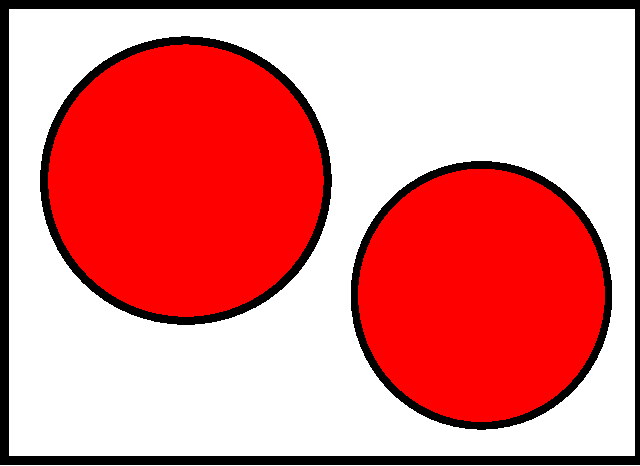
\includegraphics[width=0.3\textwidth]{figs/disjoint.pdf}
  \caption{%
    Två mängder.
    Bild:~\cite{Wikipedia2013Set}.
  }\label{fig:Disjunkt}
\end{figure}

Vi kan nu skapa mängder och tala om vilka element de innehåller, men hur kan vi
jämföra två mängder?
Hur vet vi om två mängder är lika?
\begin{definition}\label{def:Mangdlikhet}\index{mängd!likhet}\index{likhet}
  Vi säger att två mängder \(A\) och \(B\) är \emph{lika} om varje element i
  \(A\) även tillhör \(B\) och varje element i \(B\) även tillhör \(A\).
  Om \(A\) och \(B\) är lika skriver vi \(A=B\), annars skriver vi \(A\neq
  B\).
\end{definition}
\begin{exercise}\label{XrcLikhetMangd}
  Undersök vad detta innebär, vilka mängder är egentligen lika?
  Är \(\{1,2,3\}\) lika med \(\{1,1,3,3,2,3,2,1\}\)?
\end{exercise}
\begin{exercise}
  I inledning sades att en mängd kan innehålla andra mängder.
  En mängd \(X\) som tillhör en mängd \(M\) är då ett element som alla andra i
  mängden \(M\).
  Om \(X=\{1,2\}\) och \(M=\{X, 2, 3\}=\{\{1,2\},2,3\}\), vilka av följande
  utsagor är sanna och vilka är falska: 
  \(1\in M\), \(2\in M\) och \(3\in M\) samt \(\{1\}\in M\),
  \(\{2\}\in M\) och \(\{1,2\}\in M\).
\end{exercise}
\begin{exercise}\label{XrcBeskrivaTommaMangden}
  På hur många sätt kan man egentligen matematiskt beskriva den tomma
  mängden?
\end{exercise}

Vi fortsätter med ett annat viktigt begrepp, disjunktionen.
\begin{definition}\label{def:Disjunkt}\index{disjunkt}
  Två mängder \(A\) och \(B\) sägs vara \emph{disjunkta} om varje element i
  \(A\) ej är ett element i \(B\).
\end{definition}
\begin{exercise}
  Om \(A\) och \(B\) är mängder, betyder det samma sak att \(A\neq B\) som
  att \(A\) och \(B\) är disjunkta?
\end{exercise}
Mängderna i \cref{fig:Disjunkt} är disjunkta medan mängderna 
i \cref{fig:IckeDisjunkt} inte är det.
\begin{figure}
  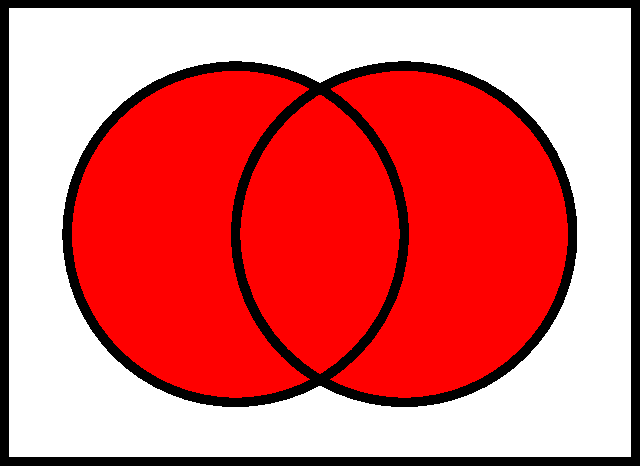
\includegraphics[width=0.3\textwidth]{figs/union.pdf}
  \caption{%
    Två icke disjunkta mängder.
    Bild:~\cite{Wikipedia2013Set}.
  }\label{fig:IckeDisjunkt}
\end{figure}


%%%%%%%%%%%%%%%%%%%%%%%%%%%%%%%%%%%%%%%%%%%%
% OPERATIONER PÅ MÄNGDER
%%%%%%%%%%%%%%%%%%%%%%%%%%%%%%%%%%%%%%%%%%%%
\section{Operationer på mängder}%
\label{sec:Mangdoperationer}
Efter att ha tittat på vad en mängd är och hur vi kan avgöra om
två mängder är lika ska vi nu titta på hur vi kan skapa nya mängder genom att
kombinera mängder som vi redan har.

\begin{definition}\label{def:Union}\index{union}
  Låt \(A\) och \(B\) vara mängder.
  Vi låter mängden \(A\cup B\) av alla element i \(A\) och alla element i
  \(B\) kallas för \emph{unionen} av \(A\) och \(B\).
  Det vill säga, \(A\cup B = \{x\colon x\in A\tor x\in B\}\).
\end{definition}
Detta illustreras med ett Venndiagram i \cref{fig:Union}.
\begin{figure}
  % XXX typeset set union figure with tex
  % XXX use eps format for figure
  \begin{minipage}{0.3\textwidth}
    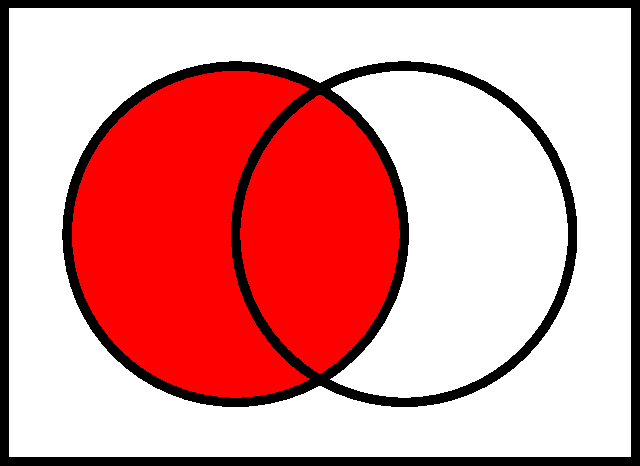
\includegraphics[width=\textwidth]{figs/A.pdf}
    \subcaption{Mängden \(A\).}
  \end{minipage}
  \hfill
  \begin{minipage}{0.3\textwidth}
    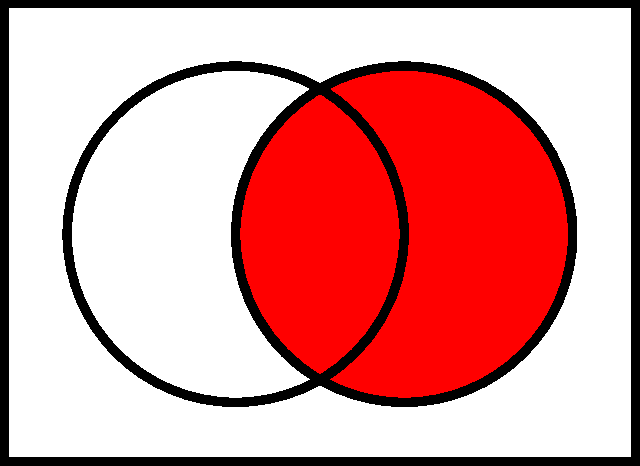
\includegraphics[width=\textwidth]{figs/B.pdf}
    \subcaption{Mängden \(B\).}
  \end{minipage}
  \hfill
  \begin{minipage}{0.3\textwidth}
    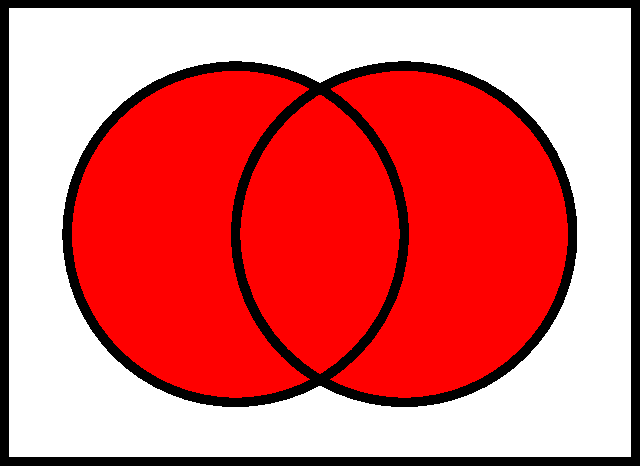
\includegraphics[width=\textwidth]{figs/union.pdf}
    \subcaption{Mängden \(A\cup B\).}
  \end{minipage}
  \caption{%
    Unionen av två mängder.
    Bild:~\cite{Wikipedia2013Set}.
  }\label{fig:Union}
\end{figure}

\begin{exercise}
  Utforska unionsoperationen, finns det några intressanta resultat om detta?
\end{exercise}

\begin{definition}\label{def:Snitt}\index{snitt}
  Låt \(A\) och \(B\) vara mängder.
  Vi låter mängden \(A\cap B\) av alla element i \(A\) som också tillhör
  \(B\) kallas för \emph{snittet} mellan \(A\) och \(B\).
  Det vill säga, \(A\cap B = \{x\colon x\in A\tand x\in B\}\).
\end{definition}
Begreppet snitt illustreras med ett Venndiagram i \cref{fig:Snitt}.
\begin{figure}
  % XXX typeset set intersection figure with tex
  % XXX use eps format for figure
  \begin{minipage}{0.3\textwidth}
    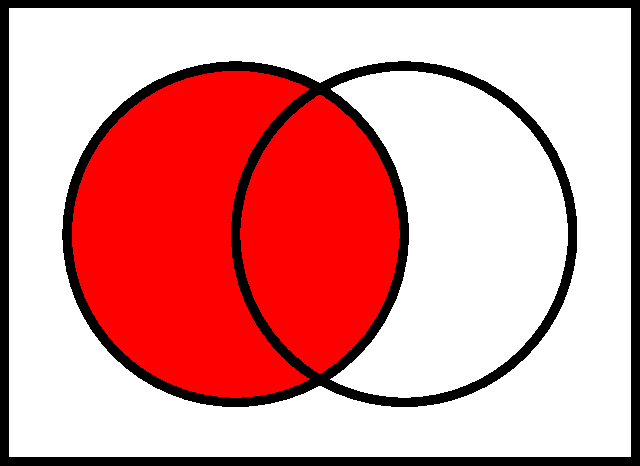
\includegraphics[width=\textwidth]{figs/A.pdf}
    \subcaption{Mängden \(A\).}
  \end{minipage}
  \hfill
  \begin{minipage}{0.3\textwidth}
    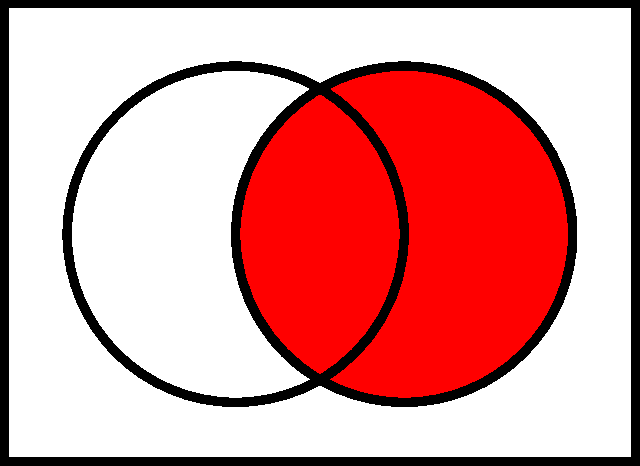
\includegraphics[width=\textwidth]{figs/B.pdf}
    \subcaption{Mängden \(B\).}
  \end{minipage}
  \hfill
  \begin{minipage}{0.3\textwidth}
    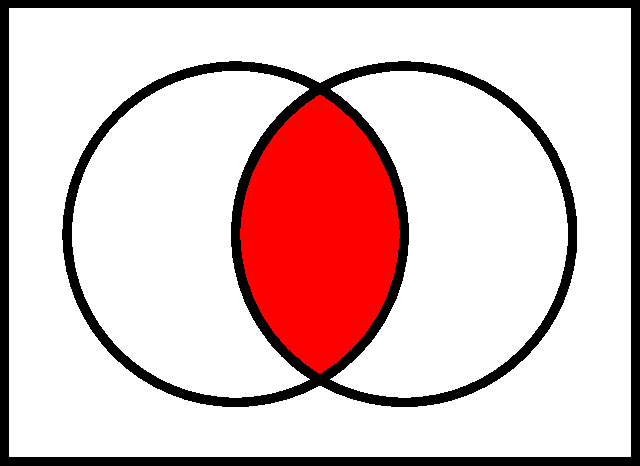
\includegraphics[width=\textwidth]{figs/intersection.pdf}
    \subcaption{Mängden \(A\cap B\).}
  \end{minipage}
  \caption{%
    Snittet av två mängder.
    Bild:~\cite{Wikipedia2013Set}.
  }\label{fig:Snitt}
\end{figure}

\begin{exercise}
  Utforska snittoperationen, finns det några intressanta resultat om detta?
\end{exercise}

\begin{exercise}
  Hur förhåller sig unions- och snittoperationerna?
  Exempelvis, spelar det någon roll om vi tar snittet av två unioner eller om 
  vi tar unionen av två snitt?
\end{exercise}

\begin{definition}\label{def:Mangddifferens}\index{differens}\index{mängd!differens}
  Låt \(A\) och \(B\) vara mängder.
  Vi låter mängden \(A\setminus B\) av alla element i \(A\) som inte tillhör
  \(B\) kallas för \emph{differensen} mellan \(A\) och \(B\).
  Det vill säga, \(A\setminus B = \{x\colon x\in A\tand x\notin B\}\).
\end{definition}
En illustration över mängderna \(A\), \(B\) och differensen \(A\setminus B\) 
ges i \cref{fig:Differens}.
\begin{figure}
  % XXX typeset set difference figure with tex
  % XXX use eps format for figure
  \begin{minipage}{0.3\textwidth}
    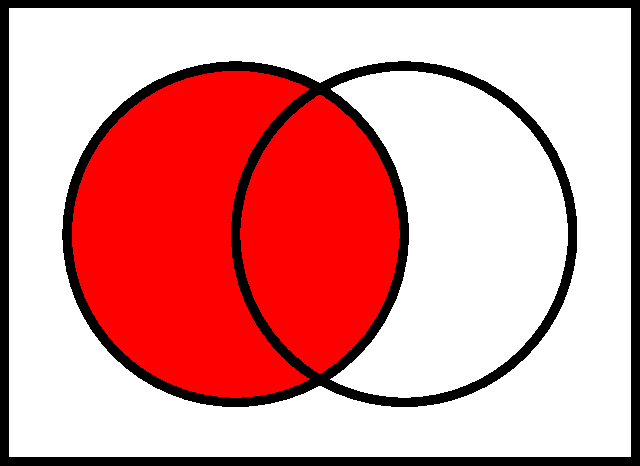
\includegraphics[width=\textwidth]{figs/A.pdf}
    \subcaption{Mängden \(A\).}
  \end{minipage}
  \hfill
  \begin{minipage}{0.3\textwidth}
    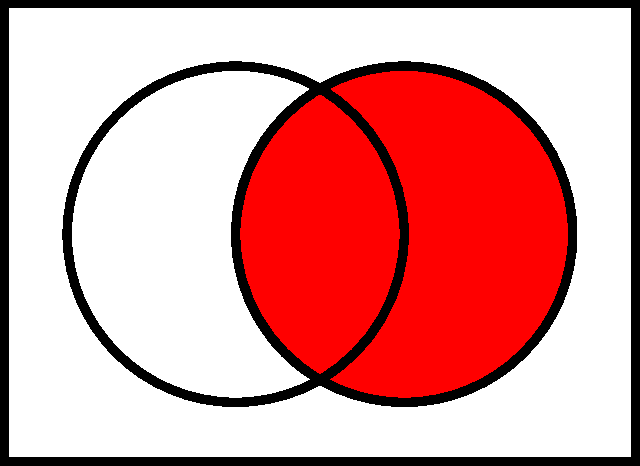
\includegraphics[width=\textwidth]{figs/B.pdf}
    \subcaption{Mängden \(B\).}
  \end{minipage}
  \hfill
  \begin{minipage}{0.3\textwidth}
    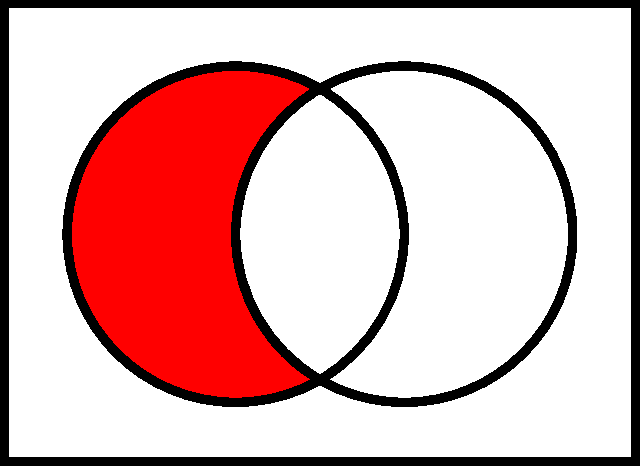
\includegraphics[width=\textwidth]{figs/A_setminus_B.pdf}
    \subcaption{Mängden \(A\setminus B\).}
  \end{minipage}
  \caption{%
    Differensen av två mängder.
    Bild:~\cite{Wikipedia2013Set}.
  }\label{fig:Differens}
\end{figure}

\begin{exercise}
  Blir det någon skillnad om vi istället definierar differensen som 
  \(A\setminus B = \{x\colon x\notin A\tand x\in B\}\)?
\end{exercise}
\begin{exercise}
  Finns det några intressanta resultat om differensen?
  Hur förhåller sig denna operation gentemot operationerna union och snitt?
\end{exercise}

\begin{definition}\label{def:KartesiskProdukt}\index{kartesisk produkt}
  Låt \(M\) och \(N\) vara mängder.
  Mängden \(\{(m,n)\colon m\in M\tand n\in N\}\) av alla ordnade par med första
  element i \(M\) och andra element i \(N\) 
  kallas för den \emph{kartesiska produkten} av \(M\) och \(N\) och skrivs
  \(M\times N\).
\end{definition}
Namnet kartesisk produkt kommer från den franske matematikern och filosofen
René Descartes (1596--1650) vars latinska namn var Renatus Cartesius.
Descartes matematiska studier gav upphov till denna typ av begrepp och därför
är den kartesiska produkten i efterhand uppkallad efter honom.

\begin{exercise}\label{xrc:Kortlek}
  Låt \(V\) vara mängden av alla valörer i en kortlek, det vill säga
  \(V=\{2,3,4,5,6,7,8,9,10,\text{knekt},\text{dam},\text{kung},\text{ess}\}\).
  Låt också \(F\) vara mängden av färger i en kortlek, det vill säga
  \(F=\{\spadesuit,\clubsuit,\heartsuit,\diamondsuit\}\).
  Vad blir \(F\times V\) och vad skulle denna mängd kunna användas för att
  representera?
\end{exercise}


%%%%%%%%%%%%%%%%%%%%%%%%%%%%%%%%%%%%%%%%%%%%
% DELMÄNGDER
%%%%%%%%%%%%%%%%%%%%%%%%%%%%%%%%%%%%%%%%%%%%
\section{Delmängder}%
\label{sec:Delmangder}
Härnäst ska vi titta på delar av mängder, eller mängder vars
element utgör en del av de element som finns i en annan mängd.
Detta är intressant för att det är inte alltid som vi är intresserade av hela
mängden, det är inte heller alltid som vi bara är intresserade av enbart ett
element.
Ibland kan det vara intressantare att titta på en del av elementen i en mängd,
och från dessa skapa en ny mängd.
Vi ger därför följande definition.

\begin{definition}\label{def:Delmangd}\index{delmängd}
  Låt \(A\) och \(B\) vara mängder.
  Vi säger att \(A\) är en \emph{delmängd} av \(B\) om varje element i \(A\)
  även tillhör \(B\).
  Vi skriver detta som \(A\subseteq B\) och utläser det som att \emph{\(A\)
  är inkluderad i \(B\)}.
  Vi kan likvärdigt skriva \(B\supseteq A\) och utläser detta som att
  \emph{\(B\) inkluderar \(A\)}.
  Om dessutom \(A\neq B\) är \(A\) en \emph{äkta} eller \emph{proper
  delmängd} av \(B\) och detta skrivs \(A\subset B\) respektive
  \(B\supset A\).
\end{definition}
I \cref{fig:Delmangd} illustreras begreppet genom ett Venndiagram.
\begin{figure}
  % XXX typeset set complement figure with tex
  % XXX use eps format for figure
  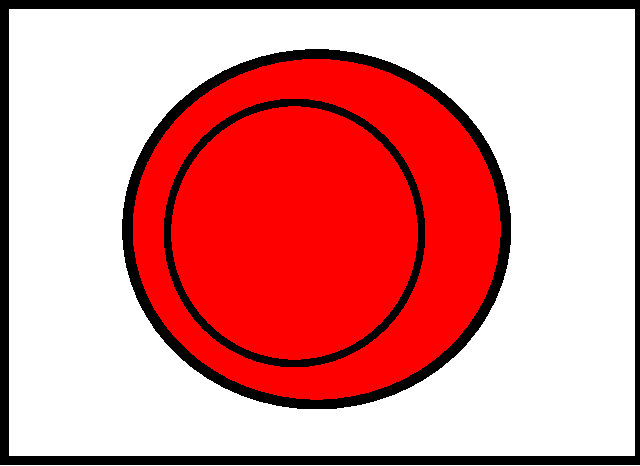
\includegraphics[width=0.3\textwidth]{figs/subset.pdf}
  \caption{%
    Två mängder, där den ena är inkluderad av den andre.
    Bild:~\cite{Wikipedia2013Set}.
  }\label{fig:Delmangd}
\end{figure}

\begin{exercise}
  Vad skulle det innebära om \(A\) är en delmängd av \(B\) och \(B\) är en
  delmängd av \(A\), det vill säga \(A\subseteq B\) och \(B\subseteq A\)?
  Är detta ens möjligt?
  Det är faktiskt så att det är en vanlig bevismetod inom matematiken att
  först visa \(A\subseteq B\) och sedan visa \(B\subseteq A\).
\end{exercise}

Vi fortsätter med en annan definition med koppling till delmängdsbegreppet.
\begin{definition}\label{def:Komplement}\index{komplement}
  Låt \(A\) vara en delmängd till mängden \(B\).
  Vi kallar mängden \(A^\complement = B\setminus A\) för \emph{komplementet}
  till \(A\) i mängden \(B\).
\end{definition}
Begreppet illustreras med ett Venndiagram i \cref{fig:Komplement}.
\begin{figure}
  % XXX typeset set complement figure with tex
  % XXX use eps format for figure
  
\includegraphics[width=0.3\textwidth]{figs/complement.pdf}
  \caption{%
    Komplementet till en delmängd.
    Bild:~\cite{Wikipedia2013Set}.
  }\label{fig:Komplement}
\end{figure}

\begin{exercise}
  Vad är det för skillnad mellan begreppen komplement och differens?
\end{exercise}

\begin{example}
  Låt \(M=\{1,2,3\}\) och \(A=\{1,2\}\) vara två mängder.
  Då har vi att \(A\subseteq M\), det vill säga \(A\) är en delmängd till
  \(M\), och faktiskt \(A\subset M\), det vill säga \(A\) är en äkta delmängd
  till \(M\).
  Vi har dessutom att komplementet till \(A\) är \(A^\complement =
  M\setminus A = \{3\}\).
\end{example}

Nu när vi har delmängder till en mängd \(M\), då kan det vara skönt att ha ett
enkelt notationssätt för mängden av alla delmängder till \(M\).
Denna mängd som innehåller alla delmängder till \(M\) som element kallas
\emph{potensmängd} och definieras härnäst.
\begin{definition}\label{def:Potensmangd}\index{potensmängd}
  Låt \(M\) vara en mängd.
  Vi kallar mängden av alla delmängder till \(M\) för \emph{potensmängden}
  av \(M\).
  Vi betecknar potensmängden till \(M\) som \(\powerset(M)\).
\end{definition}
\begin{exercise}
  Undersök hur potensmängden av en mängd \(M\) förhåller sig till mängden
  \(M\) själv.
\end{exercise}


%%%%%%%%%%%%%%%%%%%%%%%%%%%%%%%%%%%%%%%%%%%%
% RELATIONER
%%%%%%%%%%%%%%%%%%%%%%%%%%%%%%%%%%%%%%%%%%%%
\section{Relationer}\label{Relationer}

Vi ska nu titta på hur vi kan upprätta relationer mellan
elementen i en mängd.
I tidigare avsnitt har vi redan stött på en relation --- likheten mellan två
mängder.

\begin{definition}\label{def:BinarRelation}\index{relation}\index{binär 
    relation}
  En \emph{binär relation} \(R\) på en mängd \(M\) är en delmängd till den
  kartesiska produkten \(M\times M\).
  Om \((x,y)\in M\times M\) tillhör \(R\) skriver vi \(x\mathop R y\) som 
  utläses
  \emph{\(x\) är relaterat till \(y\) via \(R\)}.
\end{definition}

\begin{remark}\label{RelationDelmangdTillKartesiskProdukt}
  Mängden \(R\) är följaktligen en delmängd till den kartesiska produkten
  \(M\times M\).
\end{remark}

Enligt denna definition skulle likhetsrelationen mellan mängder vara en
relation på mängden av alla mängder och två mängder i denna mängd är relaterade
om de uppfyller kraven i \cref{def:Mangdlikhet}.
Vi ska titta på ett mindre abstrakt exempel.
\begin{example}
  Låt \(S\) vara mängden av alla personer som är skrivna på en adress i
  Sverige.
  Två personer \(p\in S\) och \(q\in S\) är relaterade via relationen \(G\)
  om de bor på samma gata.
  Om \(p\) bor på \enquote{Gatuvägen 1, 123\,45 Kommunen} och \(q\) bor på
  \enquote{Gatuvägen 3, 123\,45 Kommunen}, då gäller att \(p\mathop G q\) 
  eftersom att båda bor på \enquote{Gatuvägen}.

  Vi kan då också beskriva \(G\) på följande vis.
  Låt \(V_i\) vara mängden av alla personer som är skriva på någon väg \(i\).
  Då är \(G\) unionen av \(V_i\times V_i\) för alla vägar \(i\) i Sverige.
\end{example}

\begin{exercise}
  Använd mängderna som definieras i \cref{xrc:Kortlek} och definiera en
  relation för någon dessa.
  Inspiration: Du kan utgå från ditt favoritkortspel och definiera en eller
  flera lämpliga relationer mellan kort eller mängder av kort.
\end{exercise}


%%%%%%%%%%%%%%%%%%%%%%%%%%%%%%%%%%%%%%%%%%%%
% EKVIVALENSKLASS
%%%%%%%%%%%%%%%%%%%%%%%%%%%%%%%%%%%%%%%%%%%%
\subsection{Ekvivalensrelation och ekvivalensklass}
Vi ska nu titta på en speciell typ av relation --- ekvivalensrelationen.
Ekvivalensrelationen har en särskild struktur för hur element är relaterade
till varandra.
Den har sitt namn från att den påminner om likhetsbegreppet som vi tagit upp
tidigare.

\begin{definition}\label{def:Ekvivalensrelation}\index{ekvivalensrelation}\index{relation!ekvivalensrelation}
  En binär relation \(R\) på en mängd \(M\) som uppfyller att
  \begin{enumerate}
    \item för alla \(x\in M\) gäller att \(x\mathop R x\) (reflexivitet),
    \item för alla \(x,y\in M\) gäller att om \(x\mathop R y\) då gäller även
      \(y\mathop R x\) (symmetri),
    \item för alla \(x,y,z\in M\) gäller att om \(x\mathop R y\) och \(y\mathop 
      R z\)
      då gäller även att \(x\mathop R z\) (transitivitet),
  \end{enumerate}
  kallas för \emph{ekvivalensrelation}.
\end{definition}
\begin{exercise}
  Undersök vilka relationer du känner till som är reflexiva, symmetriska och
  transitiva, och följaktligen är ekvivalensrelationer.
\end{exercise}

En ekvivalensrelation \emph{partitionerar} en mängd \(M\) i disjunkta
delmängder kallade partitioner.
Dessa partitioner utgörs av något som brukar
kallas för ekvivalensklasser. %, som är disjunkta delmängder av mängden \(M\).
\begin{definition}\label{def:Ekvivalensklass}\index{ekvivalensklass}\index{ekvivalensrelation!ekvivalensklass}
  Låt \(R\) vara en ekvivalensrelation definierad på mängden \(M\).
  Om \(a\) är ett element i \(M\), då kallar vi mängden
  \(\{x\in M\colon x\mathop R a\}\) för \emph{ekvivalensklassen} för \(a\) och 
  betecknar denna som \([a]_R\), elementet \(a\) sägs vara en 
  \emph{representant} för ekvivalensklassen.
\end{definition}
Om det är klart under vilken relation ekvivalensklassen gäller räcker det med
att skriva \([a]\) istället för \([a]_R\).

På samma sätt som att det går att skapa en partition genom att införa en
ekvivalensrelation på mängden går det också att skapa en ekvivalensrelation på
mängden genom att partitionera den.

\begin{example}
  Låt \(F\) vara mängden av alla fåglar.
  Vi inför en relation \(A\) där två fåglar \(x\) och \(y\) är relaterade via
  \(A\) om de tillhör samma fågelart.
  Är detta en ekvivalensrelation?
  Om \(x\) är en berguv (\emph{Bubo bubo}), då måste \(x\mathop A x\) eftersom 
  att \(x\) tillhör samma fågelart som sig själv.
  Således är relationen reflexiv.
  Om \(x\) är en berguv och om \(x\mathop A y\), då måste även \(y\) vara en 
  berguv och följaktligen \(y\mathop A x\).
  Relationen är därför symmetrisk.
  Om \(x\) är en berguv och \(x\mathop A y\), då måste \(y\) vara en berguv.
  Om dessutom \(y\mathop A z\) måste \(z\) också vara en berguv.
  Eftersom både \(x\) och \(z\) är berguvar gäller att \(x\mathop A z\).
  Då är relationen transitiv.
  Relationen uppfyller kraven för en ekvivalensrelation och måste
  därför vara en ekvivalensrelation.

  Eftersom att relationen \(A\) är en ekvivalensrelation innebär det att den
  partitionerar mängden \(F\) av alla fåglar.
  Varje partition, eller ekvivalensklass, är en mängd av alla fåglar inom
  samma art.
  Exempelvis är mängden av alla berguvar en ekvivalensklass.
\end{example}

\begin{figure}
  % XXX typeset set partition figure with tex
  % XXX use eps format for figure
  
\includegraphics[width=5cm]{figs/set_partition.pdf}
  \caption{%
    En mängd (hela cirkeln) som är partitionerad i sex delmängder.
    Varje delmängd (färg) representerar en ekvivalensklass.
  }\label{fig:setPartition}
\end{figure}

Mängden av alla ekvivalensklasser hos \(M\) under relationen \(\sim\)
brukar betecknas \(M/\!\sim\) och kallas för \emph{kvotmängden av \(M\)
och \(\sim\)}\index{kvotmängd}.
Om \(m\) är ett element i \(M\), då är \([m]_\sim\) ett element i kvotmängden
\(M/\!\sim\).


%%%%%%%%%%%%%%%%%%%%%%%%%%%%%%%%%%%%%%%%%%%%
% AVBILDNINGAR
%%%%%%%%%%%%%%%%%%%%%%%%%%%%%%%%%%%%%%%%%%%%
\section{Avbildningar}
Vi ska nu införa ett annat väldigt centralt begrepp inom matematiken.
Vi ska titta på avbildningar, eller funktioner som kanske är det mer kända 
namnet.
Vi börjar med att definiera vad en funktion är.

\begin{definition}\label{def:Avbildning}\index{avbildning}\index{funktion}
  Låt \(A\) och \(B\) vara mängder.
  En \emph{funktion}, eller \emph{avbildning}, \(f\colon A\to B\) tilldelar
  till varje \(a\in A\) ett välbestämt \(b\in B\).
  Vi skriver \(f(a)=b\) eller \(a\mapsto b\) och säger att \(a\)
  \emph{avbildas} på \(b\) eller att \(b\) är \emph{bilden} av \(a\).
  Mängden \(A\) sägs vara funktionens \emph{definitionsmängd} och mängden
  \(B\) sägs vara funktionens \emph{värdemängd}.
\end{definition}
\begin{remark}
  Notera att varje funktion \(f\colon A\to B\) ger en funktionsgraf \(G_f\)
  som är en delmängd till den kartesiska produkten \(A\times B\).
  Det vill säga, \(G_f = \{(a,b)\in A\times B\colon f(a)=b\}\).
  Då är \((a,b)\in G_f\) om \(f(a)=b\), eller \(a\mapsto b\).
\end{remark}
\begin{example}
  Låt \(A=\{1,2,3\}\) och \(B=\{x,y,z\}\) vara mängder.
  Vi låter \(f\colon A\to B\) vara en funktion från \(A\) till \(B\).
  Vi låter \(1\mapsto x\), \(2\mapsto z\) och \(3\mapsto y\).
  Vi har då exempelvis att \(2\) avbildas på \(f(2)=z\).
\end{example}

\begin{exercise}
  Skulle en funktion kunna ses som en relation?
\end{exercise}

I de flesta fall är det inte lämpligt att lista alla avbildningarna för
funktionen, det vill säga ge dess funktionsgraf, som vi gjorde ovan.
Istället är det bättre att ge en beskrivning av hur elementen ska avbildas.
Vi ska illustrera med två exempel.
\begin{example}
  Låt \(M\) vara mängden av alla människor i Sverige och \(P\) vara mängden
  av alla geografiska platser på jorden.
  Låt \(p\colon M\to P\) vara en avbildning från \(M\) till \(P\).
  Vi avbildar då varje människa i \(M\) på den geografiska plats i \(P\) där
  den föddes.
\end{example}
\begin{example}
  Låt \(f\colon M\to M\) vara en avbildning från mängden
  \(M=\{0,1,2,3,\ldots\}\) till sig själv, och låt \(x\) avbildas på
  \(f(x)=x+1\).
\end{example}

Vi ska nu införa en egenskap för avbildningar.
Vi vill kunna beskriva en funktion som avbildar element på ett särskilt vis.
\begin{definition}\label{def:Injektiv}\index{injektiv}
  Låt \(f\) vara en funktion från en mängd \(A\) till en mängd \(B\).
  Vi säger att \(f\) är \emph{injektiv} om för varje \(x\in A\) och \(y\in
  A\) gäller att om \(f(x)=f(y)\) då är även \(x=y\).
\end{definition}
\begin{example}\label{ex:Surjektiv}
  Låt \(A=\{1,2,3\}\) och \(B=\{a,b\}\) vara mängder samt låt \(f\) vara en
  funktion från \(A\) till \(B\).
  Vi låter \(f(1)=a\), \(f(2)=b\) och \(f(3)=b\).
  Då är \(f\) inte injektiv eftersom att \(f(2)=f(3)\) men \(2\neq 3\).
\end{example}
\begin{example}\label{ex:Injektiv}
  Låt \(A=\{1,2\}\) och \(B=\{a,b,c\}\) vara mängder samt låt \(f\) vara en
  funktion från \(A\) till \(B\).
  Vi låter \(f(1)=a\) och \(f(2)=b\).
  Då är \(f\) injektiv eftersom att det för alla element \(x\in A\) gäller
  att om \(f(x)=f(y)\) då är \(x=y\).
\end{example}

En annan injektion illustreras i \cref{fig:Injektion}.
\begin{figure}
  % XXX typeset injection figure with tex
  \begin{minipage}{0.3\textwidth}
    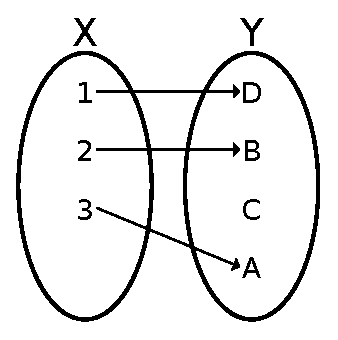
\includegraphics[width=\textwidth]{figs/injection.eps}
    \subcaption{%
      Injektion.
    }\label{fig:Injektion}
  \end{minipage}
  \hfill
  \begin{minipage}{0.3\textwidth}
    % XXX typeset surjection figure with tex
    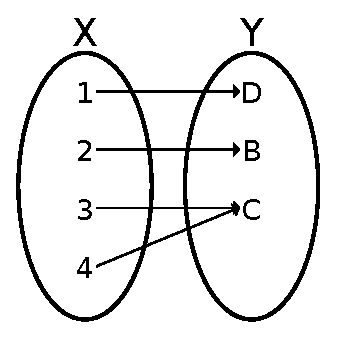
\includegraphics[width=\textwidth]{figs/surjection.eps}
    \subcaption{%
      Surjektion.
    }\label{fig:Surjektion}
  \end{minipage}
  \hfill
  \begin{minipage}{0.3\textwidth}
    % XXX typeset bijection figure with tex
    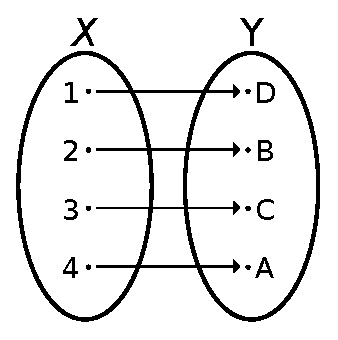
\includegraphics[width=\textwidth]{figs/bijection.eps}
    \subcaption{%
      Bijektion.
    }\label{fig:Bijektion}
  \end{minipage}
  \caption{%
    Exempel på funktioner som är injektiv, surjektiv respektive bijektiv 
    (injektiv och surjektiv).
    Bilder:~\cite{Wikipedia2013Injection}.
  }
\end{figure}

Vi ska införa en till egenskap likt den ovan.
\begin{definition}\label{def:Surjektiv}\index{surjektiv}
  Låt \(f\) vara en funktion från en mängd \(A\) till en mängd \(B\).
  Vi säger att \(f\) är \emph{surjektiv} om det för varje \(b\in B\)
  existerar ett \(a\in A\) sådant att \(b=f(a)\).
\end{definition}
\begin{example}
  Funktionen \(f\) i \cref{ex:Surjektiv} är surjektiv eftersom att
  det för varje element \(y\in B\) finns ett element i \(x\in A\) sådant
  att \(f(x)=y\).
\end{example}
\begin{example}
  Funktionen \(f\) i \cref{ex:Injektiv} är ej surjektiv eftersom att
  det finns ett element i \(B\), nämligen \(c\), sådant att
  \(f(x)\neq c\) för alla \(x\in A\).
\end{example}

I \cref{fig:Surjektion} illustreras ytterligare en surjektion.

\begin{definition}
  En avbildning som är både injektiv och surjektiv sägs vara
  \emph{bijektiv}\index{bijektiv}.
\end{definition}
\begin{exercise}
  Vad ändra mängderna i \cref{ex:Injektiv,ex:Surjektiv} för att dessa ska vara 
  bijektiva?
\end{exercise}

En bijektiv funktion illustreras i \cref{fig:Bijektion}.

%%%%%%%%%%%%%%%%%%%%%%%%%%%%%%%%%%%
% KARDINALITET
%%%%%%%%%%%%%%%%%%%%%%%%%%%%%%%%%%%
\section{Kardinalitet}
Vi kan avgöra om två mängder är lika genom att undersöka om alla
element finns med i båda mängderna, om de gör det så är mängderna lika.
Om det däremot saknas element kan vi i nuläget inte säga mycket mer än att
mängderna är olika.
Det kan dock vara intressant att kunna se hur två disjunkta mängder förhåller
sig till varandra.
Till exempel genom att bestämma hur stora de är.

När vi avgör hur stort någonting är, med avseende på antal, brukar vi räkna
antalet objekt.
Om vi exempelvis skulle avgöra hur många personer vi ser just nu börjar vi med
att peka på en person och säga \emph{ett}, peka på en annan person och säga
\emph{två}, och så vidare tills att vi har pekat på samtliga personer vi kan se.
Det vi egentligen gör när vi räknar på detta vis är att upprätta en avbildning
från talen \(1,2,3,\ldots\) till objekten vi räknar.
Vi kan utifrån denna idé definiera storleken för mängder, kallad en mängds
\emph{kardinalitet}, på följande vis.
\begin{definition}\label{def:Kardinalitet}\index{kardinalitet}
  Om \(A\) och \(B\) är mängder säger vi att de har samma \emph{kardinalitet}
  om det finns en bijektiv avbildning mellan \(A\) och \(B\).
  Vi skriver då att \(\card A = \card B\) eller \(|A| = |B|\).
  Om \(A\) har samma kardinalitet som mängden \(\{1,2,3,\ldots,n\}\) för
  något naturligt tal \(n\) skriver vi \(|A| = n\).
  Den tomma mängden \(\emptyset\) har kardinalitet \(|\emptyset| = 0\).
\end{definition}

\begin{example}
  Mängderna \(M=\{a,b,c\}\) och \(N=\{1,2,3\}\) har samma kardinalitet,
  nämligen \(3\).
  Detta eftersom att avbildningen \(f\colon M\to N\) sådan att \(f(a)=1\),
  \(f(b)=2\) och \(f(c)=3\) är bijektiv.
\end{example}

Anledningen till att vi definierar kardinalitet på detta vis är för att det är 
detta vi faktiskt gör när vi räknar, vi ställer upp en bijektion till en 
delmängd av de naturliga talen \(\N\).
Denna formulering är dock mer generell då vi inte låser oss till de naturliga 
talen.
Detta är viktigt då antalet element i mängden blir oändligt, men trots att de 
är oändligt stora vill vi fortfarande kunna jämföra dem.
Det var just detta som Cantor gjorde, och vi har redan i inledningen nämnt
några av de resultat som han kom fram till.

\ifdraft{}{%
  \part{Tal och aritmetik}
}
\chapter{De naturliga talen}\label{DeNaturligaTalen}

\lettrine{D}{e naturliga talen} är de tal som vi använder för att ordna
och räkna saker.
Talen \(1,2,3,\ldots\) är naturliga tal och det är dessa tal som människan
använt längst i historien.
Talet noll kom väldigt sent i historien, så sent som på 800-talet i Indien,
medan de andra talen använts sedan årtusenden tillbaka i tiden.
Vi ska ändå ta med talet \(0\) bland våra naturliga tal.
Mängden av naturliga tal betecknas \(\N\), det vill säga
\(\N=\{0,1,2,3,\ldots\}\).
Då dessa tal funnits länge i människans historia har de också betraktats som
självklara, så självklara att den tyske matematikern Leopold Kronecker 
(1823--1891) sade \enquote{Den käre Gud har skapat de hela talen, allt annat är 
  människans verk}~\cite[egen översättning]{Kline1990mtf3}.

Under 1800-talet blev dock matematikerna uppmärksamma på att det behövdes en
stadigare grund att bygga matematiken på.
Det gick inte längre att anta talen som självklara.
Hittills hade de naturliga talen (detta kapitel), heltalen 
(\cref{ch:Heltalen}) och de reella talen (\cref{ch:Reella}) ansetts 
vara självklara.
Men nu började självklarheten att ifrågasättas.

I detta kompendium kommer grunden att läggas först och sedan fortsätter vi
vår väg uppåt.
Det vill säga, vi börjar med de naturliga talen och går sedan vidare till de
hela talen, de rationella talen och slutligen de reella talen.
Att döma av det historiska förloppet grundades matematiken egentligen i omvänd
ordning.
Det vill säga, de reella talen grundades först.
Sedan se rationella talen, de hela talen och sist de naturliga talen.
%De reella talen var först att grundas, de grundades på de rationella talen.
%De rationella talen grundades därefter på heltalen.
%Heltalen grundades därefter på de naturliga talen.
%Slutligen grundades de naturliga talen genom de axiom som tas upp i detta
%kapitel.
%Analogt kan sägas att taket på huset byggdes innan grunden var lagd och
%väggarna resta.
Vi ska nu i kommande avsnitt titta närmare på de axiom som ligger till grund
för de naturliga talen.


%%%%%%%%%%%%%%%%%%%%%%%%%%%%%%%%%%%
% PEANOS AXIOM
%%%%%%%%%%%%%%%%%%%%%%%%%%%%%%%%%%%
\section{Peanos axiom för de naturliga talen}
Under 1800-talets slut och början av 1900-talet grundades de delar
av matematiken som redan använts sedan årtusenden tillbaka.
De naturliga talen fick sin axiomatiska grund när Richard Dedekind (1831--1916)
år 1888 publicerade ett antal axiom för de naturliga talen.
Året efter publicerade dock Giuseppe Peano (1858--1932) en förbättring av dessa
axiom och det är Peanos förbättrade axiom som godtagits och används idag,
om än i lite annorlunda formulering.

%Vi ska även se i \cref{sec:vonNeumannNaturliga} att Peanos axiom
%faktiskt kan härledas ur mängdteorin och att mängdteorin därför kan användas
%som fundamental teori för matematiken.
%Dedekind och Peanos axiom kan ändå användas som grund för de naturliga talen,
%men istället för att vara axiom blir de satser som kan härledas i mängdteorin.

Vi ska nu titta på Peanos axiom för de naturliga talen.
Börja med att släppa taget om allt du tror dig känna till om matematiken.
När du fortsätter efter denna mening ska din \enquote{matematikvärld} vara helt 
tom.
Därefter kan du fylla den med axiomen alltefter de presenteras i texten.
Vi börjar nu med det första axiomet.
\begin{axiom}\label{ax:NaturligaAxiomNoll}
  \(0\) är ett naturligt tal. 
\end{axiom}
Det första axiomet, \cref{ax:NaturligaAxiomNoll}, säger helt enkelt att det
finns åtminstone ett naturligt tal.
Det säger ingenting mer om \(0\) än att det är ett naturligt tal och
vi vet inte ännu vilka egenskaper som nollan besitter.
Detta är allt som nu finns i vår matematikvärld -- \enquote{noll är ett 
  naturligt tal}.
Vi går vidare till nästa axiom.

\begin{axiom}\label{ax:NaturligaAxiomEfterfoljare}
  För alla naturliga tal \(a\) existerar en efterföljare betecknad \(S(a)\)
  som är ett naturligt tal.
\end{axiom}
För ett naturligt tal \(n\), låter vi dess efterföljare betecknas med \(S(n)\).
På samma sätt låter vi \(S(S(n))\) beteckna efterföljaren till efterföljaren
till \(n\), och så vidare.
Notera att vi vet ännu inte vad som menas med en efterföljare.
Det enda vi vet är att alla naturliga tal har en efterföljare som är ett
naturligt tal.
Vi kan därmed fylla upp vår matematikvärld med en lång rad efterföljare och
efterföljare till efterföljare och så vidare.
\begin{axiom}\label{ax:NaturligaAxiomEjCirkular}
  För alla naturliga tal \(n\) gäller att \(0\) inte är dess efterföljare.
\end{axiom}
Vi kommer att återkomma till de två senaste axiomen.
Men låt oss först gå vidare med vad vi menar med likhet och att två naturliga
tal är lika.
Vi betecknar likhet med tecknet \(=\).
\begin{axiom}[Reflexivitet]\label{ax:NaturligaAxiomReflexivitet}
  För alla naturliga tal \(n\) gäller att \(n\) är lika med sig själv.
  Detta betecknas \(n=n\).
\end{axiom}
Vi kan nu också konstatera i vår matematikvärld att \(0=0\), och vi vet att
\(S(0)=S(0), S(S(0)) = S(S(0)), \ldots, S(S(\ldots S(0))) = S(S(\ldots
S(0)))\).
\begin{axiom}[Symmetri]\label{ax:NaturligaAxiomSymmetri}
  För alla naturliga tal \(a\) och \(b\) gäller att om \(a\) är lika med
  \(b\) då är även \(b\) lika med \(a\).
  Det vill säga, om \(a=b\) då är \(b=a\).
\end{axiom}
\begin{axiom}[Transitivitet]\label{ax:NaturligaAxiomTransitivitet}
  För alla naturliga tal \(a,b\) och \(c\) gäller att
  om \(a=b\) och \(b=c\) då är \(a=c\).
\end{axiom}
\begin{axiom}[Slutenhet under likhet]\label{ax:NaturligaAxiomSlutenhet}
  För alla naturliga tal \(a\) gäller att om \(a=b\) för något \(b\) då måste
  \(b\) också vara ett naturligt tal.
\end{axiom}
Axiomen~\ref{ax:NaturligaAxiomReflexivitet},~\ref{ax:NaturligaAxiomSymmetri},~\ref{ax:NaturligaAxiomTransitivitet} 
och~\ref{ax:NaturligaAxiomSlutenhet}
behandlar begreppet likhet (\(=\)).
Axiom~\ref{ax:NaturligaAxiomReflexivitet} säger att ett naturligt tal måste
vara lika med sig självt.
Denna egenskap kallas reflexivitet\index{reflexivitet}.
Axiom~\ref{ax:NaturligaAxiomSymmetri} säger att om ett naturligt tal är lika
med ett annat, då måste även omvändningen gälla.
Denna egenskap kallas symmetri\index{symmetri}.
Axiom~\ref{ax:NaturligaAxiomTransitivitet} säger att om vi får en kedja med
likheter, då måste ändarna av kedjorna vara lika.
Exempelvis, om \(a=b\) och \(b=c\) får vi att \(a=b=c\) och \(a=c\) måste då
gälla.
Denna egenskap kallas transitivitet\index{transitivitet}.
Axiom~\ref{ax:NaturligaAxiomSlutenhet} säger att om ett naturligt tal är lika
med någonting, då måste detta någonting också vara ett naturligt tal.
Denna egenskap kallas slutenhet\index{slutenhet}, hur vi än använder likhet kan
vi inte komma utanför de naturliga talen.
Vi vet nu hur begreppet likhet och \(=\) ska fungera och vad det betyder.

Vi ska nu introducera ytterligare ett axiom som vi vill kombinera med
tidigare axiom.
\begin{axiom}\label{ax:NaturligaAxiomInjektion}
  För alla naturliga tal \(a\) och \(b\) gäller att om deras efterföljare är
  lika måste även \(a\) och \(b\) vara lika.
  Det vill säga, om \(S(a)=S(b)\) då är \(a=b\).
\end{axiom}
Vi ska nu gå tillbaka till \cref{ax:NaturligaAxiomEfterfoljare} och
\cref{ax:NaturligaAxiomEjCirkular}.
Axiom~\ref{ax:NaturligaAxiomInjektion} säger att två olika tal kan inte ha 
samma efterföljare.
Detta betyder att vi inte kan få exempelvis grenstruktur eller ''öglor''.
Utan strukturen som måste uppstå är en linje där varje naturligt tal är en 
efterföljare till ett unikt annat naturligt tal -- med undantag för noll 
(\(0\)) som enligt \cref{ax:NaturligaAxiomEjCirkular} inte är efterföljare 
till något naturligt tal.
Axiom~\ref{ax:NaturligaAxiomEfterfoljare} säger att ett naturligt tals 
efterföljare alltid är ett naturligt tal och att en sådan alltid existerar.
Dessa två axiom säger tillsammans med \cref{ax:NaturligaAxiomInjektion} att
det finns oändligt många naturliga tal.
Om vi har ett naturligt tal kan vi alltid ta dess efterföljare enligt 
\cref{ax:NaturligaAxiomEfterfoljare}, men oavsett hur många efterföljare 
vi tar kommer vi enligt \cref{ax:NaturligaAxiomEjCirkular} aldrig tillbaka 
dit vi startade vid \(0\).
Vi vet att inget naturligt tal kan ha \(0\) som efterföljare, men \(S(0)\) då?
Om vi låter \(S(S(0))\) ha \(S(0)\) som efterföljare, då får vi en ögla trots
att det inte har \(0\) som efterföljare.
Därför behöver vi \cref{ax:NaturligaAxiomInjektion} som säger att då måste
\(S(S(0))\) och \(0\) vara samma naturliga tal -- vilket inte är sant och
följaktligen kan vi inte få några öglor.

Vi tittar nu på det sista axiomet.
\begin{axiom}[Induktionsaxiomet]\label{ax:NaturligaAxiomInduktion}
  Låt \(M\) vara en samling av objekt sådan att \(0\) tillhör \(M\) och har
  egenskapen att det för alla naturliga tal \(n\) gäller att om \(n\) tillhör
  samlingen \(M\) då tillhör även efterföljaren \(S(n)\) samlingen \(M\).
  Då innehåller \(M\) alla naturliga tal.
\end{axiom}
Det sista axiomet, \cref{ax:NaturligaAxiomInduktion}, beskriver
induktionsprincipen, de naturliga talen i sig och även mängden av alla
naturliga tal.
Det säger att om \(0\) tillhör en samling och efterföljaren till varje
naturligt tal i samlingen finns med, då innehåller mängden alla
naturliga tal.
Noll (\(0\)) är ett naturligt tal, då finns efterföljaren \(S(0)\) också med.
Eftersom att efterföljaren \(S(0)\) till \(0\) är ett naturligt tal, då måste
även \(S(S(0))\) vara med i denna samling.
Då säger vi att samlingen måste innehålla alla naturliga tal.
Det följer också från detta axiom att alla naturliga tal är på formen
\(S(S(\ldots S(0)))\).
Det är detta axiom som ligger till grund för bevismetoden induktion, därav
axiomets namn.
\begin{exercise}
  Genom diskussion jämför induktionsaxiomet,
  \cref{ax:NaturligaAxiomInduktion}, med hur induktionsbevis från
  \cref{ch:Mangder} genomförs.
\end{exercise}

Vi ska nu införa några välbekanta symboler.
\begin{definition}\label{def:NaturligaBeteckningar}
  Låt följande symboler beteckna de olika efterföljarna.
  \begin{equation*}
    1 = S(0),\quad
    2 = S(1),\quad
    3 = S(2),\quad
    \ldots
  \end{equation*}
  Låt dessutom \(\N=\{0,1,2,3,\ldots\}\) beteckna mängden av alla naturliga
  tal.
\end{definition}
\begin{remark}
  Märk väl att \(1,2\) och \(3\) enbart utgör symboler för
  \[
  S(0),S(S(0))\text{ respektive }S(S(S(0))).
  \]
  Vi vet inte hur dessa förhåller sig till varandra genom addition och
  multiplikation eftersom vi inte vet vad addition och multiplikation är
  ännu.
  Vi vet inte ens om dessa objekt som symbolerna representerar går att räkna.
  Ännu utgör dessa bara en oordnad ansamling av symboler.
\end{remark}

% TODO fixa definition av S^n(0) = S(S(...S(0)))
Vi ska nu göra en definition som kommer att förenkla vår notation avsevärt.
Denna definition använder faktiskt induktionsprincipen från induktionsaxiomet.
\begin{definition}\label{def:Efterfoljarpotenser}
  Låt \(S^0(0) = 0\).
  Om \(S^n(0)\) är definierad för något naturligt tal \(n\), då låter vi
  \(S^{S(n)}(0) = S(S^n(0))\).
\end{definition}
\begin{example}
  Vi ska titta närmare på det naturliga talet \(3=S^3(0)\).
  Vi har att \(0=S^0(0)\) och \(1=S(0)\), men då måste \(S(0)=S(S^0(0))\).
  Enligt \cref{def:Efterfoljarpotenser} är detta samma sak som
  \(S^{S(0)}(0)=S^1(0)\).
  Vi har också att \(2=S(S(0))\).
  På samma sätt som tidigare får vi att \(S(S(0))=S(S^1(0))\) och vi kan nu
  fortsätta med att konstatera att detta är lika med \(S^{S(1)}(0)=S^2(0)\).
  Vi kan nu använda detta resultat för att se att \(3=S(S(S(0)))\) faktiskt
  är \(S^3(0)\).
\end{example}


%%%%%%%%%%%%%%%%%%%%%%%%%%%%%%%%%%%%%
% VON NEUMANNS KONSTRUKTION
%%%%%%%%%%%%%%%%%%%%%%%%%%%%%%%%%%%%%
\section{Von Neumanns konstruktion av de naturliga talen}
\label{sec:vonNeumannNaturliga}
\dots


%%%%%%%%%%%%%%%%%%%%%%%%%%%%%%%%%%%%%
% ARITMETIK
%%%%%%%%%%%%%%%%%%%%%%%%%%%%%%%%%%%%%
\section{Aritmetik}
\index{aritmetik}
Ordet aritmetik kommer från grekiskans \emph{\ibygr{a)riqmo)s}},
som betyder tal, och \emph{\ibygr{a)riqmhtikh)}}, som betyder konsten att
räkna~\cite{OED2013arithmetic}.
Aritmetiken kan beskrivas som läran om att kombinera tal.
De delar av aritmetiken vi ska behandla i detta avsnitt är operationerna
addition (\(+\)) och multiplikation (\(\cdot\)).
Det vill säga, vi ska i detta avsnitt bestämma hur man räknar med de naturliga
talen.

Innan vi går vidare till att titta på addition och multiplikation behöver vi en
definition.
\begin{definition}\index{binär operation}
  En \emph{binär operation}\index{binär operation} \(\diamond\) på en mängd
  \(M\) är en funktion \(\diamond\colon M\times M\to M\) som tar två
  element \(x\) och \(y\) i \(M\) och parar dessa med ett element
  \(\diamond(x,y)\) i \(M\).
  Vanligtvis betecknas \(\diamond(x,y)\) med \(x\diamond y\).
  Det vill säga, \((x,y)\mapsto x\diamond y\).
\end{definition}


%%%%%%%%%%%%%%%%%%%%%%%%%%%%%%%%%%%%%
% ADDITION
%%%%%%%%%%%%%%%%%%%%%%%%%%%%%%%%%%%%%
\subsection{Addition}
Den första av de aritmetiska operationerna vi ska ta upp är addition.
Den definition vi använder oss av i detta kompendium är samma definition som
gavs av Peano år 1889.
Peanos definition av addition bygger även den på induktionsprincipen och kan
därför till en början kanske upplevas lite underlig och svårförståelig, men vi
ska diskutera den efteråt.
\begin{definition}[Summa]\label{def:NaturligaSumma}\index{summa}\index{term}\index{\(+\)}
  För varje par av naturliga tal \(a\) och \(b\) definieras en \emph{summa}
  \(a+b\) som är ett naturligt tal.
  Delarna \(a\) och \(b\) av en summa kallas för summans \emph{termer}.
  Vi definierar först
  \begin{equation}
    \label{eq:AdditionNoll}
    a+0 = a.
  \end{equation}
  Om summan \(a+b\) är definierad låter vi
  \begin{equation}
    \label{eq:AdditionRekursion}
    a+S(b) = S(a+b).
  \end{equation}
\end{definition}
Den första delen av definitionen är tämligen enkel.
Allt \cref{eq:AdditionNoll} säger är att om vi adderar noll från höger till
ett tal så får vi talet självt.
Det vill säga, det händer ingenting vid addition med noll från höger.
Detta är dock väldigt viktigt, och vi kommer att se varför alldeles strax. 

Den andra delen kan upplevas lite svårare.
Det \cref{eq:AdditionRekursion} säger är att ett tal adderat med efterföljaren
till ett annat är samma sak som efterföljaren till de båda talens summa.
Men hur hjälper det oss?
Det visas lättast med ett exempel.
\begin{example}
  Vi vill finna summan för talen \(2\) och \(3\).
  Alla tal kan skrivas som en kedja av efterföljare till noll, vi vet från
  \cref{def:NaturligaBeteckningar} att \(2=S(S(0))\) och \(3=S(S(S(0)))\).
  Om vi skriver summan \(2+3\) på formen från
  \cref{eq:AdditionRekursion} har vi \(2+S(S(S(0)))=S(2+S(S(0)))\).
  Men då fick vi ett nytt uttryck \(2+S(S(0))\) som är på samma form, summan
  av ett tal och efterföljaren till ett tal.
  Om vi använder \cref{eq:AdditionRekursion} igen får vi
  \(S(2+S(S(0)))=S(S(2+S(0)))\).
  Nu har vi återigen ett uttryck på samma form.
  Upprepning ger oss \(S(S(2+S(0)))=S(S(S(2+0)))\).
  Nu fick vi dock inte en summa av ett tal och en efterföljare, utan
  vi fick summan av ett tal och noll.
  Men vi vet ju från \cref{eq:AdditionNoll} att \(2+0=2\) och då får vi
  \(S(S(S(2)))\).
  Det är just detta som gör \cref{eq:AdditionNoll} så viktig, förr eller
  senare kommer vi fram till en summa där ena termen är noll och då måste vi
  veta vad det är.
  Utöver detta vi vet också att \(2=S(S(0))\), om vi sätter in detta får vi
  \(S(S(S(S(S(0)))))\) som vi enligt definition betecknar med \(5\).
  Följaktligen är \(2+3=5\).
\end{example}

Denna typ av återupprepande användning av sig själv kallas för
\emph{rekursion}\index{rekursion}.

\begin{exercise}
  Visa att om \(a\) är ett naturligt tal, då är \(a+1=S(a)\).
\end{exercise}
\begin{exercise}
  Visa att om \(a\) och \(b\) är naturliga tal, då är \(a+b=S^b(a)\).
\end{exercise}

Notera att \(a+0\) per definition är lika med \(a\), detta säger tyvärr
ingenting om \(0+a\).
\begin{exercise}
  Är \(0+a\) också lika med \(a\)?
  Bevisa ditt påstående.
\end{exercise}

Om vi studerar summan ser vi att \(+\) är en binär operation på mängden av
naturliga tal.
Vi kallar denna operation för \emph{addition}.
\begin{definition}[Addition]\label{def:NaturligaAddition}\index{addition}\index{naturliga 
    tal!addition}
  Additionsoperatorn \(+\) är en funktion \(+\colon\N\times\N\to\N\) sådan att
  varje par av naturliga tal \((a,b)\) avbildas på summan \(a+b\), som är
  ett naturligt tal som vi finner genom \cref{def:NaturligaSumma}.
\end{definition}



%%%%%%%%%%%%%%%%%%%%%%%%%%%%%%%%%%%%%
% IDENTITETSELEMENT
%%%%%%%%%%%%%%%%%%%%%%%%%%%%%%%%%%%%%
\subsection{Identitetselementet}
När vi nu sett nollans speciella betydelse är det dags att ge dess viktiga
egenskap ett namn.
Detta gör vi i följande definition.
\begin{definition}\index{identitetselement}%\index{enhet}
  Givet en mängd \(M\) med en definierad binär operation \(\diamond\colon 
  M\times M\to M\).
  Ett element \(e\) kallas \emph{identitetselement} om det för alla element
  \(x\) i mängden uppfyller att \(x\diamond e=e\diamond x=x\).
\end{definition}
\begin{example}
  Det naturliga talet \(0\) är det additiva identitetselementet för de
  naturliga talen.
\end{example}
Man kan nu undra varför vi vill ha en sådan definition enbart för nollan?
Anledningen är att det finns andra tal bland de naturliga talen som beter
precis som nollan, fast för en annan operation än addition.
Vi kommer att stöta på ett identitetselement till i nästa avsnitt.


%%%%%%%%%%%%%%%%%%%%%%%%%%%%%%%%%%%%%
% MULTIPLIKATION
%%%%%%%%%%%%%%%%%%%%%%%%%%%%%%%%%%%%%
\subsection{Multiplikation}
Multiplikation är den andra aritmetiska operationen vi ska titta på i detta
kapitel.
Även definitionen av multiplikation är den Peano gav år 1889.
Dessutom bygger även den på rekursion, precis som definitionen för addition.
\begin{definition}[Produkt]\label{def:NaturligaProdukt}\index{produkt}\index{faktor}\index{\(\cdot\)}
  För varje par av naturliga tal \(a\) och \(b\) definierar vi en
  \emph{produkt} \(a\cdot b\) som är ett naturligt tal.
  %Det vill säga \((a,b)\in\N\times\N\) och \(a\cdot b\in\N\), och alltså
  %\(\cdot\colon\N\times\N\to\N\) där \((a,b)\mapsto a\cdot b\).
  Delarna \(a\) och \(b\) av en produkt kallas för produktens \emph{faktorer}.
  Vi definierar först
  \begin{equation}
    a\cdot 0 = 0.
  \end{equation}
  Om produkten \(a\cdot b\) är definierad låter vi
  \begin{equation}
    a\cdot S(b) = a+(a\cdot b).
  \end{equation}
  Produkten \(a\cdot b\) skrivs vanligen som \(ab\).
\end{definition}

Likt summan ger även produkten en binär operation.
\begin{definition}[Multiplikation]\label{def:NaturligaMultiplikation}\index{multiplikation}\index{naturliga 
    tal!multiplikation}
  Multiplikationsoperatorn \(\cdot\) är en funktion
  \(\cdot\colon\N\times\N\to\N\) sådan att varje par av naturliga tal
  \((a,b)\) avbildas på produkten \(a\cdot b\), som är ett naturligt tal som
  vi finner genom \cref{def:NaturligaProdukt}.
  Denna operation kallar vi för \emph{multiplikation}.
\end{definition}

\begin{exercise}
  Vilket element är identitetselementet för multiplikation av de naturliga
  talen?
  Visa att så är fallet.
\end{exercise}
\begin{exercise}
  Visa att om \(a\) och \(b\) är naturliga tal, då är \[a\cdot b =
  \underbrace{a+a+\cdots+a}_b.\]
\end{exercise}
\begin{exercise}
  Visa att \(0\cdot a = 0\).
  Notera att \(a\cdot 0\) per definition är lika med \(0\), \(0\cdot a = 0\)
  fordrar dock ett bevis.
\end{exercise}


%%%%%%%%%%%%%%%%%%%%%%%%%%%%%%%%%%%%%
% LIKHET OCH OLIKHET
%%%%%%%%%%%%%%%%%%%%%%%%%%%%%%%%%%%%%
\section{Likhet och olikhet}
Det är nu dags att introducera ett sätt att jämföra tal som ej är
lika.
Vi har redan sett likhet, som vi betecknade med \(=\) och utläste \emph{är lika
med}.
Likheter är väldigt intressanta, men det finns många saker som inte är lika.
Exempelvis har vi de naturliga talen, de är oändligt många och inget av dem är
lika med något annat.
Därför definierar vi här en annan relation på de naturliga talen.

\begin{definition}[Olikhet]\index{olikhet}\index{naturliga 
    tal!olikhet}\index{<}\index{\(\leq\)}\index{>}\index{\(\geq\)}
  Låt \(a\) och \(b\) vara naturliga tal.
  Då säger vi att \(a\) är \emph{mindre än eller lika med} \(b\) om det finns
  ett naturligt tal \(n\) sådant att \(a+n=b\), vi skriver detta som
  \(a\leq b\).
  Vi kan också säga att \(b\) är \emph{större än eller lika med} \(a\) och
  beteckna detta genom \(b\geq a\).
  Om vi ej tillåter \(n\) att vara noll, då skriver vi \(a<b\)
  respektive \(b>a\).
  Vi utläser dessa som \(a\) är \emph{strikt mindre än} \(b\)
  respektive \(b\) är \emph{strikt större än} \(a\).
\end{definition}

\begin{example}
  Vi kan nu säga att \(0<1<2<3\) och så vidare.
  Det vill säga, vi har nu infört en form av ordning av de naturliga talen.
\end{example}

\begin{example}
  Låt \(x\) vara ett naturligt tal sådant att \(0<x\) och \(x<5\), det vill
  säga \(0<x<5\).
  Vi menar då att \(x\) kan vara något av talen \(1,2,3\) eller \(4\).
\end{example}

\begin{exercise}
  Är \(<\), \(\leq\), \(>\) och \(\geq\) relationer?
\end{exercise}


%%%%%%%%%%%%%%%%%%%%%%%%%%%%%%%%%%%%%
% EGENSKAPER FÖR ADDITION
%%%%%%%%%%%%%%%%%%%%%%%%%%%%%%%%%%%%%
\section{Additionens algebraiska egenskaper}

% XXX Ange referens för al-jabr
Ordet algebra kommer från arabiskans \emph{al-jabr} genom Muhammad
ibn M\={u}s\={a} al-Khw\={a}rizm\={\i}s (ca. 780-ca. 850) bok \emph{Al-Kit\={a}b
al-mukhta\d{s}ar f\={\i} h\={\i}s\={a}b al-\u{g}abr wa'l-muq\={a}bala}, på
svenska \emph{Den sammanfattande boken om beräkning genom komplettering och
  balansering}\footnote{%
  Egen översättning från \enquote{The Compendious Book on
  Calculation by Completion and Balancing}.
}.
Ordet \emph{al-jabr} betyder ordagrant \emph{återställande}.
Algebra kan beskrivas som matematikens studium av operationer och regler.
Vi ska nu titta närmare på hur den aritmetiska operationen addition beter sig.

Innan vi tittar på additionens algebraiska egenskaper behöver vi några
hjälpsatser.
Vi börjar med en mycket enkel hjälpsats som säger att om man adderar talet ett
till ett tal får man dess efterföljare.

\begin{lemma}\label{NaturligaAdderaEtt}
  Om \(a\) är ett naturligt tal, då är \(a+1\) dess efterföljare.
\end{lemma}
\begin{proof}
  Om vi tittar på additionen \(a+1\) har vi per definition att \(a+1=a+S(0)\).
  Från \cref{eq:AdditionRekursion} får vi att \(a+S(0)=S(a+0)\).
  Vi har från \cref{eq:AdditionNoll} att \(a+0=a\).
  Vi får då att
  \begin{equation}\label{eq:NaturligaAdderaEtt}
    a+1 = a+S(0) = S(a+0) = S(a).
  \end{equation}
  Således är \(a+1\) efterföljaren \(S(a)\) till \(a\).
\end{proof}

\begin{example}
  Om vi vidare tittar på additionen \(a+2\) har vi att
  \begin{equation*}
    a+2 = a+S(1) = S(a+1).
  \end{equation*}
  Vi har från \cref{NaturligaAdderaEtt} att \(a+1=S(a)\) och vi får att
  \begin{equation*}
    a+2=S(S(a))=(a+1)+1.
  \end{equation*}
\end{example}

Vi kan nu formulera en vidareutveckling av resultatet 
i \cref{NaturligaAdderaEtt}.
Vi ger vidareutvecklingen genom följande hjälpsats.
\begin{lemma}\label{lem:NaturligaAdderaN}
  Om \(a\) och \(n\) är naturliga tal gäller att
  \begin{equation}
    a+n=S^n(a).
  \end{equation}
\end{lemma}
\begin{proof}
  Vi har enligt \cref{def:NaturligaBeteckningar} att \(n=S^n(0)\).
  Då har vi att \(a+n=a+S^n(0)\).
  Enligt \cref{eq:AdditionRekursion} är \(a+S^n(0) = S(a+S^{n-1}(0))\), där
  \(n-1\) får beteckna det naturliga tal sådant att \(S(n-1)=n\).
  Men enligt \cref{eq:AdditionRekursion} är \(a+S^{n-1}(0)=S(a+S^{n-2}(0))\),
  där \(n-2\) är det naturliga tal sådant att \(S^2(n-2)=n\).
  Vi har nu att \[a+n=S(S(a+S^{n-2}(0)))=S^2(a+S^{n-2}(0)).\]
  Således har vi \(S^k(a+S^{n-k}(0))\) för \(k\leq n\).
  När \(k=n\) får vi \(S^n(a+S^{n-n}(0)) = S^n(a+0) = S^n(a)\).
\end{proof}

\begin{exercise}
  Visa att \(S^a(S^b(0)) = S^{b+a}(0)\).
\end{exercise}

Vi kan nu börja titta på vilka egenskaper som addition har.
En fråga som vi kan ställa oss, spelar det någon roll i vilken ordning vi
adderar?
Spelar det någon roll om vi adderar först \(1\) och \(2\) och sedan adderar
\(3\)?
Följande sats besvarar just den frågan.
\begin{theorem}[Associativitet]\label{thm:NaturligaAssociativitet}\label{thm:NaturligaAdditionAssociativ}\index{associativitet}\index{naturliga 
    tal!associativitet}
  Om \(a,b\) och \(c\) är naturliga tal, då gäller att \(a+(b+c)=(a+b)+c\).
\end{theorem}
\begin{proof}
  Vi börjar med att titta på \(a+(b+c)\).
  Enligt \cref{lem:NaturligaAdderaN} har vi att \(b+c=S^c(b)\).
  Enligt \cref{def:NaturligaBeteckningar} är \(b=S^b(0)\) och vi får
  att \(b+c=S^c(S^b(0))\).
  Vi har då kvar \(a+(b+c)=a+S^c(S^b(0))\).
  Enligt \cref{lem:NaturligaAdderaN} igen har vi
  \begin{equation}\label{eq:NaturligaAssociativ1}
    a+S^c(S^b(0))=S^c(S^b(a))=S^c(S^b(S^a(0))).
  \end{equation}

  Vi fortsätter med att kolla på \((a+b)+c\).
  Då har vi \(a+b=S^b(a)\) och således
  \begin{equation}\label{eq:NaturligaAssociativ2}
    S^b(a)+c=S^c(S^b(a))=S^c(S^b(S^a(0))).
  \end{equation}

  Vi ser att \cref{eq:NaturligaAssociativ1} och
  \cref{eq:NaturligaAssociativ2} är lika och således har vi även att
  \[a+(b+c)=(a+b)+c.\]
\end{proof}

\begin{example}
  Vi vill addera talen \(1,2\) och \(3\) genom \(1+2+3\).
  Enligt \cref{thm:NaturligaAssociativitet} spelar det ingen roll om vi
  först adderar \(1+2=3\) och sedan adderar \(3\), det vill säga \(3+3=6\),
  eller om vi först adderar \(2+3=5\) och sedan adderar \(1+5=6\).
  Som vi ser är \((1+2)+3=3+3=6\) och \(1+(2+3)=1+5=6\) båda lika med \(6\).
\end{example}

Vidare kan vi fråga oss, spelar det någon roll om vi adderar \(1\) med \(2\)
eller om vi adderar \(2\) med \(1\)?
Denna fråga besvaras med följande sats och bevis.
\begin{theorem}[Kommutativitet]\label{thm:NaturligaKommutativitet}\index{kommutativitet}\index{naturliga 
    tal!kommutativitet}
  Om \(a\) och \(b\) är naturliga tal, då gäller att \(a+b=b+a\).
\end{theorem}
\begin{proof}
  Vi har från \cref{lem:NaturligaAdderaN} att \(a+b=S^b(a)=S^b(S^a(0))\).
  Men
  \begin{equation}
    \label{eq:NaturligaKommutativ1}
    S^b(S^a(0)) =
    \underbrace{S(S(S(\cdots(S}_b(\underbrace{S(S(S(\cdots(S}_a(0)))))))))).
  \end{equation}

  På samma sätt har vi att \(b+a=S^a(b)=S^a(S^b(0))\) och
  \begin{equation}
    \label{eq:NaturligaKommutativ2}
    S^a(S^b(0)) =
    \underbrace{S(S(S(\cdots(S}_a(\underbrace{S(S(S(\cdots(S}_b(0)))))))))).
  \end{equation}

  Eftersom att \cref{eq:NaturligaKommutativ1} och
  \cref{eq:NaturligaKommutativ2} är lika måste vi ha \(a+b=b+a\).
\end{proof}

\begin{example}
  Vi vill addera talen \(1\) och \(2\).
  Enligt \cref{thm:NaturligaKommutativitet} spelar det ingen roll om vi 
  gör detta genom \(1+2\) eller \(2+1\).
  I båda fallen kommer vi fram till att \(1+2=2+1=3\).
\end{example}



%%%%%%%%%%%%%%%%%%%%%%%%%%%%%%%%%%%%%
% EGENSKAPER FÖR MULTIPLIKATION
%%%%%%%%%%%%%%%%%%%%%%%%%%%%%%%%%%%%%
\section{Multiplikationens algebraiska egenskaper}
Precis som för addition undrar vi nu hur multiplikation beter sig.
Spelar det någon roll i vilken ordning vi multiplicerar naturliga tal?
En ytterligare fråga som uppstår nu är dock: hur förhåller sig multiplikation
till addition?
Vi ska börja med att besvara denna fråga, sedan fortsätter vi med att undersöka
associativiteten och kommutativiteten som vi gjorde för addition.
\begin{theorem}[Distributivitet]\label{thm:NaturligaDistributivitet}\index{distributivitet}\index{naturliga 
    tal!distributivitet}
  Om \(a,b\) och \(c\) är naturliga tal gäller att
  \(a\cdot(b+c) = a\cdot b + a\cdot c\) och \((a+b)\cdot c = a\cdot c +
  b\cdot c\).
\end{theorem}
\begin{proof}
  Vi har först från \cref{lem:NaturligaAdderaN} att \(b+c=S^c(S^b(0))\).
  Således får vi att \(a\cdot (b+c) = a\cdot (S^c(S^b(0)))\).
  Från \cref{def:NaturligaMultiplikation} får vi då att
  \begin{align}
    \label{eq:NaturligaDistributivitet}
    \begin{split}
      a\cdot (b+c) &= a\cdot (S^c(S^b(0))) = \underbrace{a+a+\cdots+a}_{c} +
        a\cdot S^b(0) \\
        &= \underbrace{a+a+\cdots+a}_{c}+\underbrace{a+a+\cdots+a}_{b}.
    \end{split}
  \end{align}
  Om vi tittar på de enskilda delarna av uttrycket längst till höger.
  Då har vi enligt definitionen för produkten att
  \begin{align*}
    \underbrace{a+a+\cdots+a}_{b}
      &= \underbrace{a+a+\cdots+a}_{b-1}+a\cdot S(0) \\
      &= \underbrace{a+a+\cdots+a}_{b-2}+a\cdot S(1) \\
      &= \underbrace{a+a+\cdots+a}_{b-3}+a\cdot S(2) \\
      & \vdots \\
      &= a\cdot b.
  \end{align*}
  Vi har på samma sätt att
  \begin{equation*}
    \underbrace{a+a+\cdots+a}_{c} = a\cdot c.
  \end{equation*}
  Om vi använder detta i \cref{eq:NaturligaDistributivitet} får vi att
  \begin{equation*}
    a\cdot (b+c) = \underbrace{a+a+\cdots+a}_b+\underbrace{a+a+\cdots+a}_c
      = a\cdot b + a\cdot c,
  \end{equation*}
  vilket visar första delen av satsen.

  Om vi tittar på \((a+b)\cdot c\) får vi att
  \begin{equation*}
    (a+b)\cdot c = \underbrace{(a+b)+(a+b)+\cdots+(a+b)}_c.
  \end{equation*}
  Eftersom att additionen är associativ och kommutativ kan vi byta plats
  på termerna och får då
  \begin{equation*}
    \underbrace{(a+b)+(a+b)+\cdots+(a+b)}_c =
    \underbrace{a+a+\cdots+a}_c+\underbrace{b+b+\cdots+b}_c.
  \end{equation*}
  På samma sätt som ovan får vi att detta är \(a\cdot c + b\cdot c\).
  Då har vi visat att \((a+b)\cdot c = a\cdot c + b\cdot c\) och vi har visat
  satsen.
\end{proof}

\begin{exercise}
  Gäller det också att
  \(a\cdot (b_1+b_2+\cdots+b_n) =
    a\cdot b_1 + a\cdot b_2 + \cdots + a\cdot b_n\)?
\end{exercise}

Vi vet nu hur multiplikationen förhåller sig till additionen och kan då gå
vidare till att undersöka om multiplikationen har de associativa och
kommutativa egenskaperna som additionen har.
Vi börjar med associativiteten.
\begin{theorem}[Associativitet]\label{thm:NaturligaMultiplikationAssociativ}\index{associativitet}\index{naturliga 
    tal!associativitet}
  Om \(a\) och \(b\) är naturliga tal, då gäller att \(a\cdot(b\cdot
  c)=(a\cdot b)\cdot c\).
\end{theorem}
\begin{proof}
  Vi tittar först på \(a\cdot (b\cdot c)\) och får enligt definitionen för
  multiplikation att
  \begin{equation*}
    a\cdot (b\cdot c) = a\cdot (\underbrace{b+b+\cdots+b}_c).
  \end{equation*}
  Eftersom att multiplikationen är distributiv
  (\cref{thm:NaturligaDistributivitet}) får vi att
  \begin{equation}
    \label{eq:NaturligaMultAssoc1}
    a\cdot (\underbrace{b+b+\cdots +b}_c) = \underbrace{a\cdot b+a\cdot
      b+\cdots+a\cdot b}_c.
  \end{equation}

  Vi tittar nu på \((a\cdot b)\cdot c\).
  Enligt definitionen för multiplikation är
  \begin{equation}
    \label{eq:NaturligaMultAssoc2}
    (a\cdot b)\cdot c = \underbrace{a\cdot b+a\cdot b+\cdots+a\cdot b}_c.
  \end{equation}

  Eftersom att \cref{eq:NaturligaMultAssoc1} och
  \cref{eq:NaturligaMultAssoc2} är lika har vi visat satsen.
\end{proof}

\begin{theorem}[Kommutativitet]\index{kommutativitet}\index{naturliga 
    tal!kommutativitet}
  Om \(a\) och \(b\) är naturliga tal, då gäller att \(a\cdot b=b\cdot a\).
\end{theorem}
\begin{proof}
  Beviset använder induktion.
  Låt \(a\) vara ett naturligt tal.
  Vi vill visa att \(a\cdot b = b\cdot a\) för alla naturliga tal \(b\).
  För \(b=0\) är det klart att multiplikationen är kommutativ.
  För \(b=1\) har vi att
  \begin{equation}
    \label{eq:MultKommutativ1}
    a\cdot 1 = a+a\cdot 0 = a.
  \end{equation}
  Vi har också att
  \begin{equation*}
    1\cdot a = \underbrace{1+1+\cdots+1}_a.
  \end{equation*}
  Enligt \cref{NaturligaAdderaEtt} och att additionen är associativ
  (\cref{thm:NaturligaAdditionAssociativ}) får vi att
  \begin{equation}
    \label{eq:MultKommutativ2}
    \underbrace{1+1+\cdots+1}_a = S^a(0) = a.
  \end{equation}
  Eftersom att \cref{eq:MultKommutativ1} och \cref{eq:MultKommutativ2} är
  lika måste också \(a\cdot 1 = 1\cdot a\).

  Antag att multiplikationen är kommutativ för alla \(b\) mindre än \(k\).
  Vi har då att \(a\cdot k = k\cdot a\).
  Vi vill nu visa att då måste multiplikationen vara kommutativ även för
  \(b=k+1\).
  Eftersom att multiplikation är distributiv över addition
  (\cref{thm:NaturligaDistributivitet}) har vi att \(a\cdot (k+1) = a\cdot
  k + a\cdot 1\).
  Vi har redan konstaterat att \(a\cdot k = k\cdot a\) och att \(a\cdot 1 =
  1\cdot a\), och följaktligen är \(a\cdot (k+1) = a\cdot k + a\cdot 1 =
  k\cdot a + 1\cdot a\).
  Vi har från distributiviteten igen att \(k\cdot a + 1\cdot a = (k+1)\cdot
  a\).
  Således är multiplikationen kommutativ även för \(b=k+1\) och den måste
  därför vara kommutativ för alla naturliga tal.
\end{proof}
\begin{exercise}
  Vilka likheter finns mellan beviset ovan och induktionsaxiomet för de
  naturliga talen?
\end{exercise}

\begin{exercise}
  Visa att \((a+b)(c+d) = ac+ad+bc+bd\).
\end{exercise}


%%%%%%%%%%%%%%%%%%%%%%%%%%%%%%%%%%%
% ALGEBRAISKA EGENSKAPER
%%%%%%%%%%%%%%%%%%%%%%%%%%%%%%%%%%%
\section{Algebraiska egenskaper för de naturliga talen}
\label{sec:HeltalensAlgebraiskaEgenskaper}
Det är nu dags att sammanfatta de algebraiska egenskaperna för de
naturliga talen.
Vi har i tidigare avsnitt visat att de naturliga talen har följande egenskaper.

\theoremstyle{plain}
\newtheorem*{AlgebraicPropertiesNatural}{Algebraiska egenskaper för de
  naturliga talen}
\begin{AlgebraicPropertiesNatural}\label{def:HeltalenEgenskaper}
  På mängden \(\N\) av hela tal definieras två binära operationer,
  addition (\(+\)) och multiplikation (\(\cdot\)).
  För addition gäller följande:
  \begin{description}
    \item[Kommutativitet] \(a+b=b+a\) för alla \(a,b\in\N\).
    \item[Associtivitet] \((a+b)+c=a+(b+c)\) för alla \(a,b,c\in\N\).
    \item[Additivt identitetselement] Det finns ett element \(0\in\N\)
      sådant att för alla \(a\in\N\) gäller att \(0+a = a+0 = a\).
  \end{description}
  För multiplikation gäller följande:
  \begin{description}
    \item[Kommutativitet] \(a \cdot b=b \cdot a\) för alla \(a,b\in\N\).
    \item[Associtivitet] \((a \cdot b) \cdot c=a \cdot (b \cdot c)\) för
      alla \(a,b,c\in\N\).
    \item[Multiplikativt identitetselement] Det finns ett element
      \(1\in\N\) sådant att för alla \(a\in\N\) gäller att
      \(1 \cdot a = a \cdot 1 = a\).
  \end{description}
  Utöver detta gäller även
  \begin{description}
    \item[Multiplikativ distributivitet över addition]
      \(a \cdot (b+c) = (a \cdot b) + (a \cdot c)\) och
      \((b+c) \cdot a = (b \cdot a) + (c \cdot a)\) för alla reella tal
      \(a,b,c\in\N\).
  \end{description}
\end{AlgebraicPropertiesNatural}

För en djupare och mer generell behandling av dessa egenskaper rekommenderas 
läsaren till~\cite{Bartle2000itr,Grillet2007aa}.


%%%%%%%%%%%%%%%%%%%%%%%%%%%%%%%%%%%%%
% POTENSER
%%%%%%%%%%%%%%%%%%%%%%%%%%%%%%%%%%%%%
\section{Potenser}
Det kan bli tröttsamt i längden att skriva ut många faktorer i en
produkt.
För additionen kunde vi istället för att skriva \(a+a+\cdots+a\)
multiplicera \(a\) med antalet \(a\)-termer i summan, på så vis behöver vi inte
skriva ut alla \(a\)-termer utan det räcker med att vi vet vilken term och hur
många vi ska addera.
Vi vill naturligtvis kunna göra liknande för multiplikation.
Istället för att skriva ut alla \(b\)-faktorer i en produkt \(b\cdot
b\cdots b\) räcker det med att vi skriver faktorn och antalet av denna
faktor.
Då skriver vi produkten \(b\cdot b\cdots b\) med \(n\) faktorer som \(a^n\).
Detta åstadkommer vi med potenser som definieras enligt följande.
\begin{definition}
  Låt \(a\) och \(n\) vara naturliga tal.
  Låt \(a^1=a^{S(0)}=a\).
  Om \(a^n\) är definierad låter vi \(a^{S(n)}=a\cdot a^n\).
  Vi kallar \(a^n\) för en \emph{\(a\)-potens} med \emph{exponenten} \(n\).
\end{definition}
\begin{remark}
  Notera att \(a^0\) ej är definierad för något naturligt tal \(a\).
  Vi återkommer till detta i \cref{ch:Rationella} som handlar om rationella
  tal.
\end{remark}

\begin{example}
  Vi har produkten \(2\cdot 2\cdot 2\) som består av tre termer som alla är
  \(2\).
  Vi kan då skriva produkten som en \(2\)-potens, nämligen \(2^3\).
  Enligt definitionen är \(2^3=2\cdot 2^2=2\cdot 2\cdot 2^1 = 2\cdot 2\cdot
  2\).
\end{example}

\begin{example}
  Talet \(72\) kan skrivas som produkten \(8\cdot 9=2\cdot 2\cdot 2\cdot
  3\cdot 3\).
  Om vi använder potensform får vi att \(72=2^3\cdot 3^2=2^3 3^2\).
\end{example}

\begin{example}
  Talet \(4\) kan skrivas som en \(4\)-potens, nämligen \(4^1\).
  Det kan också skrivas som en \(2\)-potens, nämligen \(4=2\cdot 2=2^2\).
\end{example}


%%%%%%%%%%%%%%%%%%%%%%%%%%%%%%%%%%%%%
% RESULTAT OM POTENSER
%%%%%%%%%%%%%%%%%%%%%%%%%%%%%%%%%%%%%
\subsection{Några resultat om potenser}
Vi ska nu titta på några enkla resultat som följer av vår definition av
potenser.
En första fråga kan vara, vad händer om vi adderar två potenser?
\begin{example}\label{ex:AdderaPotenser}
  Vi vill addera potenserna \(a^n\) och \(b^m\) där \(a\) och \(b\) är
  naturliga tal och \(n\) och \(m\) är naturliga tal skilda från noll.
  Om vi adderar dem får vi
  \begin{equation*}
    a^n + b^m = \underbrace{a\cdot a\cdots a}_n + \underbrace{b\cdot
    b\cdots b}_m.
  \end{equation*}
  Vi kan inte komma särskilt mycket längre och vi kan konstatera att detta
  var ett föga intressant resultat.
\end{example}

Om vi istället testar att multiplicera två potenser.
\begin{example}\label{ex:MultipliceraPotenser}
  Vi vill multiplicera potenserna \(a^n\) och \(b^m\) där \(a\) och \(b\) är
  naturliga tal och \(n\) och \(m\) är naturliga tal skilda från noll.
  Vi får då att
  \begin{equation*}
    a^n\cdot b^m = a^n b^m = \underbrace{a\cdot a\cdots a}_n\cdot
    \underbrace{b\cdot b\cdots b}_m.
  \end{equation*}
  Detta verkar mer lovande, vad händer om \(a=b\)?

  Om \(a=b\) får vi att
  \begin{multline}
    \label{eq:MultipliceraPotenser}
    a^n b^m = a^n a^m = \underbrace{a\cdot a\cdots a}_n\cdot\underbrace{a\cdot
    a\cdots a}_m = \\
    \underbrace{a\cdot a\cdots a}_{n}\cdot a^m = a^{S^n(m)} = a^{n+m}.
  \end{multline}
\end{example}

Detta är ett intressant resultat och vi sammanfattar det som följande sats.
\begin{theorem}\label{thm:AdderaExponenter}
  Om \(a\), \(n\neq 0\) och \(m\neq 0\) är naturliga tal, då är \(a^n a^m =
  a^{n+m}\).
\end{theorem}
\begin{proof}
  Satsen följer direkt från \cref{eq:MultipliceraPotenser}.
\end{proof}

\begin{example}
  Vi vill multiplicera potenserna \(2^3\) och \(2^5\).
  Vi får då enligt \cref{thm:AdderaExponenter} att
  \begin{equation*}
    2^3 2^5 = 2^{3+5} = 2^8.
  \end{equation*}
  Om vi kontrollerar ser vi att \(2^3=8\) multiplicerat med \(2^5=32\)
  faktiskt är \(2^8=256\).
\end{example}

Eftersom att det fungerar att addera exponenterna ter det sig naturligt att
fråga om vi även kan multiplicera exponenterna och vad det skulle betyda.
\begin{example}\label{ex:MultipliceraExponenter}
  Om \(a\), \(n\neq 0\) och \(m\neq 0\) är naturliga tal kan vi skapa
  potensen \(a^{nm}\).
  Vi vet att \[nm = \underbrace{n+n+\cdots+n}_m\] och således att
  \begin{equation}
    \label{eq:MultipliceraExponenter1}
    a^{nm}=a^{n+n+\cdots+n}=\underbrace{a^n a^n\cdots a^n}_m.
  \end{equation}
  Men vi har nyss definierat potenser för att förenkla skrivandet av sådana
  produkter.
  Följaktligen får vi att
  \begin{equation}
    \label{eq:MultipliceraExponenter2}
    a^n a^n\cdots a^n = (a^n)^m.
  \end{equation}
\end{example}
Vi sammanfattar resultatet i följande sats.
\begin{theorem}
  Låt \(a\), \(n\neq 0\) och \(m\neq 0\) vara naturliga tal.
  Då gäller att \((a^n)^m = a^{nm}\).
\end{theorem}
\begin{proof}
  Satsen följer från \cref{ex:MultipliceraExponenter}.
\end{proof}

Vi har nu visat att vi har addition och multiplikation av exponenter.
Följande sats visar också att multiplikation av exponenter är distributiv över
addition av exponenter.
\begin{theorem}\label{thm:MultipliceraExponenter}
  Om \(a\), \(b\), \(n\neq 0\), \(m\neq 0\) och \(p\neq 0\) är naturliga tal,
  då är \((a^n b^m)^p = a^{np} b^{mp}\).
\end{theorem}
\begin{proof}
  Om vi tittar på vad \((a^n b^m)^p\) faktiskt betyder, så finner vi att
  \begin{equation*}
    (a^n b^m)^p = \underbrace{(a^n b^m)(a^n b^m)\cdots (a^n b^m)}_p.
  \end{equation*}
  Eftersom att multiplikation är associativ och kommutativ får vi att
  \begin{equation*}
    \underbrace{(a^n b^m)(a^n b^m)\cdots (a^n b^m)}_p =
    \underbrace{a^n a^n\cdots a^n}_p \underbrace{b^m b^m\cdots b^m}_p =
    (a^n)^p (b^m)^p.
  \end{equation*}
  Vi har från \cref{ex:MultipliceraExponenter} att \((a^n)^p(b^m)^p =
  a^{np}b^{mp}\).
  Och därför är \((a^n b^m)^p = a^{np} b^{mp}\).
\end{proof}

Vi avslutar avsnittet med ett exempel som nyttjar de båda satserna.
\begin{example}
  Vi vill multiplicera \(4^3\) och \(12^2\).
  Vi vet att \(4=2\cdot 2\), det vill säga \(4=2^2\), samt att \(12=3\cdot
  4=3\cdot 2^2\).
  Om vi använder detta och tittar på vad vi hade från början, \(4^3\) är
  således \((2^2)^3=2^{2\cdot 3}=2^6\).
  \(12^2\) blir då \((3\cdot 2^2)^2\) och således \(12^2=3^{1\cdot
  2} 2^{2\cdot 2} = 3^2 2^4\).
  Om vi multiplicerar dem får vi
  \begin{equation*}
    (\underbrace{2^6}_{4^3}\cdot \underbrace{3^2 2^4}_{12^2}) =
    2^6 2^4 3^2 = 2^{6+4} 3^2 = 2^{10} 3^2.
  \end{equation*}
\end{example}

\begin{exercise}
  Visa att addition av exponenter och multiplikation av exponenter båda är
  associativa och kommutativa operationer.
\end{exercise}


%%%%%%%%%%%%%%%%%%%%%%%%%%%%%%%%%%%%%
% VÄLORDNINGSPRINCIPEN
%%%%%%%%%%%%%%%%%%%%%%%%%%%%%%%%%%%%%
\subsection{Välordningsprincipen}
\dots

\begin{theorem}[Välordningsegenskapen hos de naturliga 
  talen]\label{def:Valordningsprincipen}\index{välordningsegenskapen}\index{naturliga 
    tal!välordningsegenskapen}
  Om en mängd \(M\subseteq\N\) är en delmängd till de naturliga talen och om
  \(M\neq\emptyset\) ej är den tomma mängden, då existerar ett element
  \(m\in M\) i \(M\) sådant att \(m\leq k\) är mindre än \(k\) för alla
  \(k\in M\) i \(M\).
\end{theorem}
\begin{proof}
  \dots
\end{proof}


%%%%%%%%%%%%%%%%%%%%%%%%%%%%%%%%%%%%%
% AVSLUTANDE REFLEKTION
%%%%%%%%%%%%%%%%%%%%%%%%%%%%%%%%%%%%%
\section{Avslutande reflektion}
Som en avslutande reflektion till detta kapitel ges följande
övningsuppgifter.
Tanken med dessa övningar är att reflektera över matematikens existens, hur den
förhåller sig till verkligheten etc.

\begin{exercise}
  Diskutera förhållandet mellan matematiken och verkligheten.
  En inledande fråga i diskussionen kan vara:
  Grundar sig matematiken i verkligheten eller är den oberoende av
  verkligheten?
  Diskutera.
\end{exercise}

\begin{exercise}
  a: Om matematiken är oberoende av verkligheten, hur kan den användas
  för att utforska och förutsäga verkligheten? Och om verkligheten såg
  annorlunda ut, skulle matematiken se likadan ut?

  b: Om matematiken grundar sig i verkligheten, hur kan den användas för att
  förutsäga verkligheten när den behöver verkligheten för att visas vara sann?
\end{exercise}


\chapter{De hela talen}
\label{ch:Heltalen}
\lettrine{V}{i är nu välbekanta} med de naturliga talen,
\(\N=\{0,1,2,\ldots\}\).
Vi har operationerna addition och multiplikation och vet hur dessa fungerar.
I detta kapitel kommer vi att utöka de naturliga talen med avseende på
addition.

Om vi adderar två tal \(a\) och \(b\) får vi ett tredje tal \(c\), vi skriver
detta som \(a+b=c\).
Det finns dock inget sätt att ta oss tillbaka till \(a\), det vill säga det
finns inget naturligt tal \(d\) sådant att \(c+d=a+b+d=a\).
Ett annat sätt att säga det på är att det finns inga naturliga tal \(n\) och
\(m\) sådana att deras summa \(n+m=0\) är lika med identitetselementet noll.
Detta är dock en väldigt intressant och önskvärd egenskap.
Vi ska förtydliga vad vi menar och ge denna egenskap ett namn.
\begin{definition}\label{def:invers}\index{invers}
  Givet en mängd \(M\) med en definierad binär operation \(\diamond\colon 
  M\times M\to M\) och ett identitetselement \(e\).
  Ett element \(b\) kallas för \emph{inversen till} ett element \(a\) om
  \(a\diamond b = b\diamond a = e\).
\end{definition}
\begin{exercise}
  Utforska inversbegreppet.
  Frågor att inspirera:
  I \cref{def:invers}, är \(a\) inversen till något element?
  Hur många inverser kan ett element ha?
  Har alla element en invers?
\end{exercise}
%\begin{remark}
%  Av inversens natur följer att om \(b\) är inversen till \(a\), då är även
%  \(a\) inversen till \(b\).
%\end{remark}

Vi ska i detta kapitel tillföra denna egenskap till additionen för de naturliga
talen.
Resultatet är vad som kallas de hela talen, och mängden av de hela talen
betecknas\footnote{Anledningen till att de betecknas med \(\Z\) är tyskans
\emph{Zahlen} som betyder tal.} \(\Z\).


%%%%%%%%%%%%%%%%%%%%%%%%%%%%%%%%%%%
% UTÖKNINGEN
%%%%%%%%%%%%%%%%%%%%%%%%%%%%%%%%%%%
\section{Utökningen av de naturliga talen}
\label{sec:HeltalensKonstruktion}
Låt oss nu skapa de hela talen.
Det enda vi har att tillgå är de naturliga talen, dessa vet vi att de
existerar och hur de fungerar.
Vi börjar med att låta mängden \(M = \N\times\N =
\{(a,b)\colon a\text{ och }b\text{ är naturliga tal}\}\) vara mängden av alla
ordnade par av naturliga tal.
\begin{example}
  Vi har exempelvis att \((1,2)\in M\) och \((2,1)\in M\) samt att
  \((1,2)\neq (2,1)\).
\end{example}

Låt oss nu införa en relation \(\sim\) på denna mängd.
Om \((a,b)\) och \((c,d)\) är ordnade par av naturliga tal, det vill säga
element i mängden \(M\), då vill vi att \((a,b)\sim (c,d)\) ska vara sant
precis när \(a+d=b+c\).
Denna relation \(\sim\) är faktiskt en ekvivalensrelation.
För att visa detta kollar vi att relationen uppfyller axiomen i
\cref{def:Ekvivalensrelation} för en ekvivalensrelation.
Additionen är kommutativ och eftersom att \(a+b=b+a\) har vi
\((a,b)\sim (a,b)\), och följaktligen är den reflexiv.
Om \((a,b)\sim (c,d)\) då är \(a+d=b+c\) och således 
\begin{align*}
  c+b &= b+c,\\
  d+a &= a+d \text{\ och\ } \\
  c+b &= d+a.
\end{align*}
Den sista ekvationen ger precis \((c,d)\sim (a,b)\).
Relationen måste då vara symmetrisk.
För att visa transitiviteten behövs följande resultat.
\begin{lemma}\label{lem:AdditionInjektiv}
  Låt \(x\) och \(y\) vara naturliga tal.
  Om \(z\) är ett naturligt tal och \(x+z=y+z\) då är \(x=y\).
\end{lemma}
\begin{exercise}
  Bevisa \cref{lem:AdditionInjektiv}.
\end{exercise}
Om \((a,b)\sim (c,d)\) och \((c,d)\sim (e,f)\), då har vi först att
\begin{equation}
  \label{eq:VisaHeltalensEkvivalensrelation1}
  a+d = b+c
\end{equation}
och sedan att
\begin{equation}
  \label{eq:VisaHeltalensEkvivalensrelation2}
  c+f=d+e.
\end{equation}
Detta ger
\begin{equation*}
  a+d+f = b+c+f = b+d+e.
\end{equation*}
Eftersom att additionen är kommutativ får vi \(a+f+d = b+e+d\) och
enligt \cref{lem:AdditionInjektiv} har vi då att \(a+f = b+e\) som
betyder att \((a,b)\sim (e,f)\).
Eftersom att relationen då även är transitiv är relationen en
ekvivalensrelation.

Vi betecknar ekvivalensklasserna på följande sätt:
Om \((a,b)\) är ett element i \(M\), då är
\([(a,b)]=\{(x,y)\in M\colon (a,b)\sim (x,y)\}\).
Det vill säga, \([(a,b)]\) innehåller alla talpar i \(M\) som uppfyller
ekvivalensrelationen med talparet \((a,b)\).
\begin{example}
  Vi har att \((0,0)\sim (1,1)\) eftersom att \(0+1 = 0+1\).
  Följaktligen har vi \([(0,0)]=[(1,1)]\) och \((1,1)\in [(0,0)]\), men
  naturligtvis även \((0,0)\in [(0,0)]\).
\end{example}
\begin{remark}
  Kom ihåg att det inte spelar någon roll om vi väljer \((0,0)\) eller
  \((1,1)\) som representant för
  ekvivalensklassen \([(0,0)]=[(1,1)]\) eftersom att det är samma
  ekvivalensklass.
\end{remark}
\begin{example}
  Vi har däremot \((0,0)\nsim (1,0)\) eftersom att \(0+0\neq 0+1\),
  och följaktligen \((1,0)\notin [(0,0)]\).
\end{example}

Låt oss nu definiera en binär operation \(+\) som vi kallar för addition och en
binär operation \(\cdot\) som vi kallar för multiplikation på mängden av
ekvivalensklasser hos \(M\).
Vi låter \([(a,b)]+[(c,d)] = [(a+c, b+d)]\) och \([(a,b)]\cdot [(c,d)] =
[(ac+bd, ad+bc)]\).
Vi måste dock visa att dessa är väldefinierade.
%\begin{proof}[Väldefinierad addition]
Om \((a,b)\sim (a^\prime, b^\prime)\) och \((c,d)\sim (c^\prime,
d^\prime)\), då vill vi visa att \((a+c, b+d)\sim (a^\prime+c^\prime,
b^\prime+d^\prime)\).
Vi har från \((a,b)\sim (a^\prime,b^\prime)\) att \(a+b^\prime =
b+a^\prime\) och från \((c,d)\sim (c^\prime,d^\prime)\) att
\(c+d^\prime=d+c^\prime\).
Om vi adderar vänsterleden i de båda ekvationerna, då måste detta vara lika
med summan av högerleden.
Det vill säga, \((a+b^\prime) + (c+d^\prime) = (b+a^\prime) +
(d+c^\prime)\).
Eftersom att additionen är associativ och kommutativ får vi att
\begin{equation*}
  a+c+b^\prime+d^\prime = b+d+a^\prime+c^\prime,
\end{equation*}
och således måste \((a+c,b+d)\sim (a^\prime+c^\prime, b^\prime+d^\prime)\).
%\end{proof}
\begin{exercise}
  Visa att multiplikationen också är väldefinierad.
\end{exercise}

\begin{example}\label{ex:HeltalAddition}
  Om vi adderar \([(1,2)]\) och \([(2,4)]\) får vi
  \begin{equation*}
    [(1,2)]+[(2,4)] = [(1+2,2+4)] = [(3, 6)] = [(0,3)].
  \end{equation*}
\end{example}
\begin{example}\label{ex:HeltalMultiplikation}
  Om vi multiplicerar \([(1,2)]\) och \([(2,4)]\) får vi
  \begin{equation*}
    [(1,2)]\cdot [(2,4)] = [(1\cdot 2 + 2\cdot 4, 1\cdot 4 + 2\cdot 2)] =
    [(10, 8)] = [(2,0)].
  \end{equation*}
\end{example}

Vi har nu objekt med egenskaperna att de beter sig som de naturliga talen, men
vi kan även addera dem för att få identitetselementet.
Identitetselementet för addition måste vara ekvivalensklassen \([(0,0)]\).
Eftersom att \([(a,b)]+[(0,0)] = [(a+0,b+0)] = [(a,b)]\) och
\([(0,0)]+[(a,b)] = [(0+a,0+b)] = [(a,b)]\) måste \([(0,0)]\)
vara identitetselementet för addition.

\begin{exercise}
  Hur skulle de naturliga talen kunna representeras med dessa objekt?
\end{exercise}

Den additiva inversen till \([(a,b)]\) är \([(b,a)]\) eftersom att
\([(a,b)]+[(b,a)]=[(a+b,b+a)]=[(a+b,a+b)]\).
Eftersom att \(0+(a+b)=0+(a+b)\) har vi enligt ekvivalensrelationen att
\((0,0)\sim (a+b,a+b)\) och därför måste de tillhöra samma ekvivalensklass.
Detta innebär att \([(a,b)]\) och \([(b,a)]\) måste vara varandras inverser
under addition.

\begin{exercise}
  Kan ett tal ha fler än en invers?
\end{exercise}

Vi sammanfattar detta avsnitt med följande definitioner.
Vi börjar med att definiera vad de hela talen är.
\begin{definition}[Heltalen]\index{heltal}
  Låt \(M=\N\times\N\) vara mängden av alla naturliga talpar och \(\sim\)
  vara ekvivalensrelationen på mängden \(M\) sådan att \((a,b)\sim (c,d)\)
  är uppfylld för elementen \((a,b)\) och \((c,d)\) i \(M\) om \(a+d=b+c\).

  Låt \(\Z = M/\!\sim = \{[(a,b)]\colon (a,b)\in M\}\) vara mängden av alla
  ekvivalensklasser för \(M\) under ekvivalensrelationen \(\sim\).
  Varje element \(n\) i \(\Z\) kallar vi ett \emph{heltal}.

  Låt också \(0\) beteckna \([(0,0)]\in\Z\), \(1\) beteckna \([(1,0)]\in\Z\)
  och \(a\) beteckna \([(a,0)]\in\Z\) för alla naturliga tal \(a\).
  Beteckna också den additiva inversen \([(0,a)]\in\Z\) till \([(a,0)]\) med
  \(-a\).
\end{definition}
De nya beteckningarna och ekvivalensklasserna visas i
\cref{fig:HeltalensEkvivalensklasser}.
\begin{figure}
  \centering
  \begin{asy}
    // Courtesy of Thomas Douillard, thomas.douillard at gmail.com
    // From Wikipedia
    // import settings
    import graph;
    size(10cm,0);
    // returns a pair representation of a relative number
    // of the equivalent class
    pair pairRepresentation(int n){//
            if(n>0){//
                    return(n,0);
            }else{//
                    return(0,-n);
            }
    }
    string nullString(real r){//
            return "";
    }
    void drawCoordinates(pair point, align align=NoAlign){//
            label("$("+string(point.x)+","+string(point.y)+")$",point,align,
              fontsize(10));
    }
    unitsize(50,50);
    int num = 5;
    int i;
    for (i=-1*num ; i<=num ; ++i) {//
            pair point = pairRepresentation(i) ;
            dot(point,red);
            // equivalence classes labelled with usual names, in blue
            label("$\mathbf{"+string(i)+"}$",point,5SW,fontsize(10)+blue);
            int j;
            for(j=abs(i);j<num;++j) {//
                    drawCoordinates(point,E);
                    pair nextpoint = point + (1,1);
                    draw(point -- nextpoint,blue+Dotted+linewidth(2));
                    dot(point,red+linewidth(5));
                    point=nextpoint;
            }
            dot(point,red);
            draw(point -- point+(0.5,0.5),blue+Dotted+linewidth(2));
            dot(point,red+linewidth(5));
            drawCoordinates(point,E);
    }
    // axes
    real decay=-0.2;
    ticks tick=RightTicks(N=0,n=1,end=false,nullString);
    xaxis("$n_1$",YEquals(decay),decay,num+1.0,tick,Arrow);
    yaxis("$n_2$",XEquals(decay),decay,num+1.0,LeftTicks(N=0,n=1,end=false,nullString),Arrow);
  \end{asy}
  \caption{%
    Ekvivalensklasser för par av naturliga tal \((n_1,n_2)\) under
    relationen \(\sim\).
    Bild:~\cite{Wikipedia2013Integer}.
  }\label{fig:HeltalensEkvivalensklasser}
\end{figure}

När vi nu vet vad ett heltal är kan det vara passande att införa aritmetiska
operationer för dem.
Vi börjar med additionen och fortsätter med multiplikationen senare.
\begin{definition}[Addition]\index{addition}\index{heltal!addition}
  Låt \(x=[(a,b)]\) och \(y=[(c,d)]\) vara heltal och \(+\) en binär
  operation på \(\Z\), kallad \emph{addition}, sådan att
  \(x+y=[(a,b)]+[(c,d)]\) är lika med \([(a+c,b+d)]\).
\end{definition}
\begin{exercise}
  I \cref{ex:HeltalAddition}, vilka tal adderades och vilket blev resultatet?
\end{exercise}
\begin{exercise}
  Är additionen kommutativ för de hela talen?
\end{exercise}
\begin{exercise}
  Är additionen associativ för de hela talen?
\end{exercise}

Nu när vi kan addera heltal är det lämpligt att vi tittar på hur vi kan jämföra
dem annat än med likhet.
Olikheter infördes med hjälp av additionen för de naturliga talen, det är inte
förvånande att vi gör detsamma för heltalen.
\begin{definition}[Olikhet]\index{olikhet}
  Låt \(x=[(a,b)]\) och \(y=[(c,d)]\) vara heltal.
  Vi säger att \(x\) \emph{är mindre än} \(y\), betecknat \(x<y\), om
  \(a+d<b+c\) enligt relationen \(<\) för de naturliga talen.
  Vi kan också säga att \(y\) \emph{är större än} \(x\) och skriver då
  \(y>x\).
  Vi säger att \(x\) \emph{är mindre än eller lika med} \(y\) om \(a+d\leq
  b+c\), detta betecknas \(x\leq y\).
  Vi kan också säga att \(y\) \emph{är större än eller lika med} \(x\) och
  betecknas \(y\geq x\).
\end{definition}

Nu när vi kan ordna de hela talen är den naturliga efterföljande definitionen
denna.
\begin{definition}\index{negativt tal}\index{positivt tal}
  Låt oss kalla ett tal mindre än noll för ett \emph{negativt} tal, och låt
  oss kalla ett tal större än noll för ett \emph{positivt} tal.
\end{definition}
Vi har nu infört olika namn för talen på båda sidorna om talet noll.
Notera att enligt denna definition är noll varken positivt eller negativt.

\begin{exercise}
  Hur ordnas de hela talen?
\end{exercise}

Nu till inverserna.
\begin{definition}\index{negation}\index{additiv invers}
  Om \(x=[(a,b)]\) är ett heltal, då är \(-x=-[(a,b)]=[(b,a)]\) dess
  \emph{additiva invers}.
  Denna kallas även för \emph{negationen} av \(x\).
\end{definition}
\begin{remark}
  Låt \(a\) och \(b\) vara heltal och \(-b\) den additiva inversen till
  \(b\).
  Normalt skriver vi \(a+(-b)\) som \(a-b\) för att spara in på några tecken.
  Vi benämner \(a-b\) som \emph{subtraktionen}\index{subtraktion} av \(b\)
  från \(a\).
  Ur en matematisk synvinkel är subtraktion inte en egen operation utan vi
  adderar den additiva inversen för \(b\) till \(a\).
\end{remark}

\begin{exercise}
  Visa att ett nollskilt naturligt tal är ett positivt tal.
\end{exercise}
\begin{exercise}
  Visa att den additiva inversen för ett nollskilt naturligt tal är ett
  negativt tal.
\end{exercise}
\begin{exercise}
  De naturliga talens ordning är \(0 < 1 < 2 < 3 < \ldots\), enligt relationen 
  \(<\) definierad för de naturliga talen.
  Gäller denna ordning även för relationen \(<\) definierad för de hela talen?
\end{exercise}

Den andra aritmetiska operationen, multiplikation, ger vi i den sista
definitionen.
\begin{definition}[Multiplikation]\index{multiplikation}\index{heltal!multiplikation}
  Låt \(x=[(a,b)]\) och \(y=[(c,d)]\) vara heltal och \(\cdot\) en binär
  operation på \(\Z\), kallad \emph{multiplikation}, sådan att
  \(x\cdot y=[(a,b)]\cdot [(c,d)]\) är lika med \([(ac+bd,ad+bc)]\).
  Vi skriver ofta \(xy\) istället för \(x\cdot y\).
\end{definition}
\begin{exercise}
  I \cref{ex:HeltalMultiplikation}, vilka tal multiplicerades och vilket
  blev resultatet?
\end{exercise}

Vi ska nu visa ett lemma som vi kommer att behöva i kommande avsnitt.
Lemmat talar om att produkten av ett helt tal och noll blir noll.
\begin{lemma}\label{lem:IngenNolldelare}
  För alla heltal \(a\) gäller att \(a\cdot 0 = 0\cdot a = 0\).
\end{lemma}
\begin{proof}
  Antag att \(a = [(b,c)]\) där \(b\) och \(c\) är naturliga tal.
  Vi har per definition att \(a\cdot 0 = [(b,c)]\cdot [(0,0)] =
  [(b\cdot 0 + c\cdot 0, a\cdot 0 + c\cdot 0)] = [(0,0)] = 0\).
  På samma sätt får vi att \(0\cdot a = [(0,0)]\cdot [(b,c)] = [(0\cdot b +
  0\cdot c, 0\cdot c + 0\cdot b)] = [(0,0)] = 0\).
\end{proof}

\begin{exercise}
  Är multiplikationen kommutativ för de hela talen?
\end{exercise}
\begin{exercise}
  Är multiplikationen associativ för de hela talen?
\end{exercise}
\begin{exercise}
  Är multiplikationen distributiv över additionen för de hela talen?
\end{exercise}


%%%%%%%%%%%%%%%%%%%%%%%%%%%%%%%%%%%
% ALGEBRAISKA EGENSKAPER
%%%%%%%%%%%%%%%%%%%%%%%%%%%%%%%%%%%
\section{Algebraiska egenskaper för de hela talen}
\label{sec:HeltalensAlgebraiskaEgenskaper}
Det är nu dags att sammanfatta de algebraiska egenskaperna för de
hela talen.
De hela talen bygger på de naturliga talen och ska vara en utökning av dessa.
Vi hade för avsikt att de hela talen skulle ha samma algebraiska egenskaper som
vi visat att de naturliga talen har.
Vi fortsätter därför härnäst med en sammanfattning av de algebraiska egenskaper
som de hela talen måste ha.
Dessa är desamma som för de naturliga talen förutom tillägget om att varje tal
\(a\) har en additiv invers \(-a\).

\theoremstyle{plain}
\newtheorem*{AlgebraicPropertiesIntegers}{Algebraiska egenskaper för de hela
  talen}
\begin{AlgebraicPropertiesIntegers}\label{def:HeltalenEgenskaper}
  På mängden \(\Z\) av hela tal definieras två binära operationer,
  addition (\(+\)) och multiplikation (\(\cdot\)).
  För addition gäller följande:
  \begin{description}
    \item[Kommutativitet] \(a+b=b+a\) för alla \(a,b\in\Z\).
    \item[Associtivitet] \((a+b)+c=a+(b+c)\) för alla \(a,b,c\in\Z\).
    \item[Additivt identitetselement] Det finns ett element \(0\in\Z\)
      sådant att för alla \(a\in\Z\) gäller att \(0+a = a+0 = a\).
    \item[Additiv invers] För alla \(a\in\Z\) finns ett element \(-a\in\Z\)
      sådant att \(a + (-a) = (-a) + a = 0\).
  \end{description}
  För multiplikation gäller följande:
  \begin{description}
    \item[Kommutativitet] \(a \cdot b=b \cdot a\) för alla \(a,b\in\Z\).
    \item[Associtivitet] \((a \cdot b) \cdot c=a \cdot (b \cdot c)\) för
      alla \(a,b,c\in\Z\).
    \item[Multiplikativt identitetselement] Det finns ett element
      \(1\in\Z\) sådant att för alla \(a\in\Z\) gäller att
      \(1 \cdot a = a \cdot 1 = a\).
  \end{description}
  Utöver detta gäller även
  \begin{description}
    \item[Multiplikativ distributivitet över addition]
      \(a \cdot (b+c) = (a \cdot b) + (a \cdot c)\) och
      \((b+c) \cdot a = (b \cdot a) + (c \cdot a)\) för alla hela tal
      \(a,b,c\in\Z\).
  \end{description}
\end{AlgebraicPropertiesIntegers}

För en mer detaljerad behandling av dessa egenskaper hänvisas läsaren till 
\cite{Bartle2000itr,Grillet2007aa}.



%%%%%%%%%%%%%%%%%%%%%%%%%%%%%%%%%%%%%%%%%%%%
% ALGEBRAISKA EGENSKAPER FÖR DE NEGATIVA TALEN
%%%%%%%%%%%%%%%%%%%%%%%%%%%%%%%%%%%%%%%%%%%%
\section{Algebraiska egenskaper för de negativa talen}
Vi är redan bekanta med de naturliga talen, och därmed också den
delen av de hela talen som motsvarar de naturliga talen.
Därför ska vi i detta avsnitt fokusera på de nya talen, de heltal \(a<0\) som
är mindre än noll -- eller de negativa talen.

Låt oss börja med ett av de fundamentala resultaten,
% (-1)a = -a
nämligen att ett heltal \(a\) multiplicerat med \(-1\) ger dess invers \(-a\).
Vi formulerar detta som en sats.
\begin{theorem}\label{thm:FaktoriseraNegativaTal}
  Låt \(a\) vara ett heltal.
  Då är \(a\) multiplicerat med \(-1\) inversen \(-a\) till \(a\).
  Det vill säga, \((-1)\cdot a = -a\).
\end{theorem}
\begin{proof}
  Vi har att \(1+(-1) = 0\).
  Om vi multiplicerar noll med ett tal får vi enlingt
  \cref{lem:IngenNolldelare} fortfarande noll.
  Följaktligen får vi att \(a(1+(-1))=0\) eftersom att vi då multiplicerar
  \(a\) med noll.
  Eftersom att multiplikation är distributiv över addition får vi då att
  \begin{equation*}
    a(1+(-1)) = 1\cdot a + (-1)a = a + (-1)a = 0.
  \end{equation*}
  Då måste \((-1)a\) vara inversen \(-a\) till \(a\).
\end{proof}
\begin{remark}
  Notera att detta och följande resultat även kan härledas direkt från
  talparskonstruktionen i \cref{sec:HeltalensKonstruktion} trots att vi
  i detta bevis väljer att använda oss av de algebraiska egenskaperna givna i
  \cref{sec:HeltalensAlgebraiskaEgenskaper}.
\end{remark}

% (-1)(-1) = (-1)^2 = 1
Vi fortsätter med kanske det mest häpnanväckande resultatet, som är en
följdsats till föregående.
\begin{corollary}\label{NegMultNegEqPos}
  Den additiva inversen \(-1\) till heltalet ett multiplicerad med sig
  själv är ett.
  Det vill säga \((-1)(-1) = 1\).
\end{corollary}
\begin{proof}
  Eftersom att \(-1\) är ett heltal följer det från
  \cref{thm:FaktoriseraNegativaTal} att om vi multiplicerar det med \(-1\)
  får vi dess invers.
  Inversen för \(-1\) är \(1\) och således har vi att \((-1)(-1)=1\).
\end{proof}

\begin{exercise}
  Om \(a\) och \(b\) är heltal, gäller då att \((-a)(-b) = ab\) för alla
  heltal \(a\) och \(b\)?
\end{exercise}

Låt oss avsluta med ett exempel om addition av två negativa tal.
\begin{example}
  % (-1)+(-1) = -2
  Om vi adderar \(-1\) och \(-1\), vad får vi då?
  Eftersom att vi adderar två lika termer kan vi skriva additionen som
  multiplikationen \(2\cdot (-1) = (-1)+(-1)\).
  Vi vet från \cref{thm:FaktoriseraNegativaTal} att ett heltal
  multiplicerat med \(-1\) är dess invers, då får vi \((-1)+(-1)=2\cdot
  (-1) = -2\).
\end{example}
\begin{example}
  Vi kan också beräkna summan \((-1)+(-1)\) genom att använda heltalens
  distributiva egenskap.
  Eftersom att \((-1)=(-1)\cdot 1\) och att multiplikation är distributiv
  över addition får vi att \((-1)+(-1) = (-1)(1+1) = (-1)(2) = -2\).
\end{example}
\begin{exercise}
  % (-1)(a+b) = (-a)+(-b)
  Om \(a\) och \(b\) är heltal,
  gäller generellt att \((-a)+(-b)=-(a+b)\)?
\end{exercise}

\begin{exercise}
  % (-1)(a-b) = (-1)(a+(-b)) = (-a)+b
  Utred vad \(-(a-b)\) egentligen betyder.
\end{exercise}


%%%%%%%%%%%%%%%%%%%%%%%%%%%%%%%%%%%%%%%%%%%%
% POTENSER
%%%%%%%%%%%%%%%%%%%%%%%%%%%%%%%%%%%%%%%%%%%%
\subsection{Potenser för heltalen}
Vi ska nu införa potenser för de hela talen, likt de vi införde för de
naturliga talen.
Vi definierar potenser enligt följande definition.
\begin{definition}
  Låt \(a\) vara ett heltal.
  Vi definierar att \(a^1=a\).
  Om \(a^{n}\) är definierat för något naturligt tal \(n > 0\), då är
  \(a^{n+1} = a\cdot a^n\).
  Vi utläser \(a^n\) som en \emph{\(a\)-potens med exponenten \(n\)}, eller 
  \emph{\(a\) upphöjt till \(n\)}.
\end{definition}

\begin{exercise}
  Utforska potenser för de hela talen.
  Finns det några intressanta resultat om dessa potenser?
  %Gäller resultaten vi visat för de naturliga talen?
\end{exercise}


\chapter{Talteori}%
\label{ch:Talteori}%\nocite{Laksov2005kou,Bartle2000itr}
\lettrine{T}{alteori är studiet} av talen, primärt de hela talen.
Ett exempel på ett mycket enkelt talteoretiskt fynd är att vartannt tal är 
jämnt och vartannat är udda; det vill säga att varje heltal \(n\) kan skrivas 
som \(n = 2k\) om det är jämnt respektive \(n = 2k+1\) om det är udda, där 
\(k\) är ett heltal.

Enligt en redogörelse av \citet{Kline1990mtf1} inleddes studiet av talen redan 
av babylonierna\footnote{%
  Babylonier är en benämning av de folk som levde i området Mesopotamien, ett 
  område mellan floderna Eufrat och Tigris i vad som idag är 
  Irak~\cite{Kline1990mtf1}.
}, vars storhetstid var mellan cirka 2500--300 f.v.t.\@
De härledde bland annat resultatet att \[1 + 2 + 4 + \cdots + 2^n = 2^n + (2^n 
- 1) = 2^{n+1} - 1.\]
% XXX Ge exempel på Pythagoreiska tripplar: a^2 + b^2 = c^2
% XXX Ta upp Diophantos
Grekerna fortsatte i sin tur att studera talen under sin storhetstid, vilken 
varade mellan cirka 600 f.v.t.\ till omkring år 300.
De mest kända grekiska matematiker och filosofer som studerade talteori är 
kanske Pythagoras\index{Pythagoras} (cirka 585--500 f.v.t.), då främst 
gemensamt med sina anhängare kända som Pythagoréerna\index{Pythagoréerna}, samt 
Euklides\index{Euklides} (omkring 300 f.v.t.).
Anledningen till att saker tillskrivs Pythagoréerna är för att de historiska 
dokument som finns tillgängliga inte skiljer på vad som åstadkommits av 
Pythagoras själv eller hans lärljungar, därför används Pythagoras och 
Pythagoréerna synonymt i de flesta texter (denna inräknad).

Bland Pythagoréernas resultat kan nämnas att
\begin{equation}
  \label{eq:pyth-square}
  n^2 + (2n + 1) = (n + 1)^2.
\end{equation}
Anledningen till detta resultat var att Pythagoréerna representerade tal som 
prickar i sanden, se figurerna~\ref{fig:pyth-triangles} 
och~\ref{fig:pyth-squares}.
\begin{figure}
  \centering
  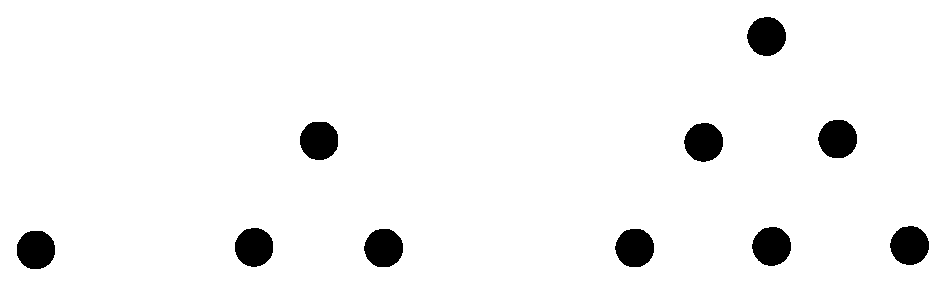
\includegraphics[width=4cm]{figs/pyth-triangles.eps}
  \caption{%
    Talen 1, 3 och 6 representerade med Pythagoreiska trianglar.
  }\label{fig:pyth-triangles}
\end{figure}
\begin{figure}
  \centering
  
\includegraphics[width=4cm]{figs/pyth-squares.eps}
  \caption{%
    Talen 1, 4 och 9 representerade med Pythagoreiska kvadrater.
  }\label{fig:pyth-squares}
\end{figure}
Tal som kunde representeras som en triangel kallade de följaktligen för 
triangulära tal\index{triangulära tal} och tal som kunde representeras som 
kvadrater kallades för kvadratiska tal\index{kvadratiska tal}.
Ett resultat som fascinerade dem var att varje kvadratiskt tal kunde 
konstrueras genom additionen av två triangulära tal.
Ett annat, det som gavs som \cref{eq:pyth-square} ovan, är hur nästa 
kvadratiska tal återfinns; \( (n+1)^2 \) är det kvadratiska tal som följer 
\(n^2\) och \(2n + 1\) är antalet prickar som måste läggas till längs kanterna.
\begin{exercise}
  Undersök om det finns ett liknande uttryck för triangulära tal.
\end{exercise}
\begin{exercise}
  För vilka triangulära tal gäller att om två triangulära tal adderas är 
  resultatet ett kvadratiskt?
\end{exercise}

Fermats och Eulers resultat som omnämndes redan i \cref{Introduktion} är ett 
mycket intressant talteoretiskt resultat.
Det är fortfarande historiskt, dock modernt i jämförelse med ovan nämnda 
resultat.
Vi kommer att behandla Fermats och Eulers satser senare i detta kapitel.

Ytterligare ett resultat, ett olöst sådant, är Goldbachs förmodan.
Denna förmodan uttalades av Chrisitan Goldbach (1690--1794)~\cite{goldbach} och 
säger att varje naturligt tal kan skrivas som en summa av primtal.
Begreppet primtal är centralt för talteorin och vi kommer strax att återkomma 
till dessa.


%%%%%%%%%%%%%%%%%%%%%%%%%%%%%%%%%%%%%%%%%%%%
% DELBARTHET
%%%%%%%%%%%%%%%%%%%%%%%%%%%%%%%%%%%%%%%%%%%%
\section{Delbarhet}
Ett av de centrala begreppen inom talteorin är delbarheten hos de hela 
talen.
Vi inleder avsnittet med att definiera vad vi menar med detta.
\begin{definition}[Delbarhet]\index{delbarhet}\index{delare}\index{äkta delare}
  Vi säger att ett tal \(a\in\Z\) delar ett tal \(b\in\Z\) om det finns ett tal 
  \(q\in\Z\) sådant att \(b = qa\).
  Vi skriver då \(a\mid b\), vilket utläses som \emph{\(a\) delar \(b\)}.
  På motsvarande sätt har vi \(a\nmid b\) för \emph{\(a\) delar inte \(b\)}.
  Om dessutom \(a\neq b\) sägs \(a\) vara en \emph{äkta delare} till \(b\).
\end{definition}
\begin{example}
  Vi har att \(2\mid 4\) eftersom att \(4 = 2\cdot 2\), två är dessutom en äkta 
  delare.
  Tre är däremot inte en delare till fyra, så \(3\nmid 4\).
  Vi har att \(3\mid 12\) eftersom att \(12 = 3\cdot 2^2\), tre är dessutom en 
  äkta delare till \(12\).
  Vi har har \(12\mid 12\) eftersom att \(12 = 1\cdot 12\), men \(12\) är dock 
  inte en äkta delare till \(12\).
\end{example}
\begin{exercise}\label{xrc:delare}
  Undersök hur olika tal delar varandra och se om ni finner något samband.
\end{exercise}

För att underlätta i kommande bevis ger vi först ett antal fundamentala lemman 
om egenskaperna för delbarhet.
\begin{lemma}\label{lem:divtransitiv}
  Om \(a\mid b\) och \(b\mid c\), då måste även \(a\mid c\).
\end{lemma}
\begin{proof}
  Låt \(b = xa\) och \(c = yb\), då måste \(c = yxa\) och följaktligen måste 
  \(a\mid c\).
\end{proof}
\begin{lemma}\label{lem:divassoc}
  Om \(a\mid b\) och \(a\mid c\), då måste \(a\mid xb + yc\) för alla heltal 
  \(x\) och \(y\).
\end{lemma}
\begin{exercise}
  Bevisa \cref{lem:divassoc}.
\end{exercise}
\begin{lemma}\label{lem:divdistnondiv}
  Om \(a\mid b\) och \(a\nmid c\), då måste \(a\nmid b+c\).
\end{lemma}
\begin{exercise}
  Bevisa \cref{lem:divdistnondiv}, ett förslag är att tillämpa 
  \cref{lem:divassoc}.
\end{exercise}
\begin{exercise}
  Diskutera och förklara varför \(3\mid 6\) men \(3\nmid 5\), \(3\nmid 2\) och 
  \(3\nmid 1\) då \(6 = 5 + 1 = 4 + 2 = 3 + 2 + 1 = 3 + 3\).
\end{exercise}
\begin{lemma}\label{lem:divnoll}
  Om \(ab\neq 0\) och \(a\mid b\) och \(b\mid a\), då måste \(a = b\) eller \(a 
  = -b\).
\end{lemma}
\begin{proof}
  Låt \(a = xb\) och \(b = ya\), då måste \(b = yxb\).
  Eftersom att \(b\neq 0\) måste \(yx = 1\) och således är \(x\) och \(y\) 
  antingen båda \(1\) eller båda \(-1\).
\end{proof}
\begin{lemma}\label{lem:divneg}
  Om \(a\mid b\), då måste \(-a\mid b\), \(-a\mid -b\) och \(a\mid -b\).
\end{lemma}
\begin{exercise}
  Bevisa \cref{lem:divneg}.
\end{exercise}
\begin{exercise}
  Diskutera innebörden av de olika lemmorna.
\end{exercise}

När vi nu är bekanta med begreppet delare ska vi introducera 
divisionsalgoritmen.
Denna ger oss ett verktyg för att dela heltal med varandra och är faktiskt den 
första typen av division som introduceras i svensk skola, den introduceras 
redan i årskurs 1--3 i grundskolan.

\begin{theorem}[Divisionsalgoritmen]\label{thm:divisionsalgoritmen}\index{divisionsalgoritmen}
  Låt \(b\) vara ett positivt heltal.
  För varje heltal \(a\) finns unika heltal \(q\) och \(r\) sådana att \[a = qb 
  + r,\] där \(0\leq r < b\).
\end{theorem}

Innan vi bevisar att algoritmen är korrekt är det lämpligt att vi bevisar ett 
antal lemman.

\begin{lemma}\label{lem:DisjunktaIntervallAvZ}
  Låt \( i_x = \{y\in\Z \colon xb\leq y < (x + 1)b\} \) beteckna ett intervall 
  för varje \(x\in\Z\).
  Då är \(i_x\) och \(i_{x'}\) disjunkta, det vill säga \(i_x\cap \i_{x'} = 
    \emptyset\).
  Deras union \(\cup_{x\in \Z} i_x = \Z\) utgör hela \(\Z\).
\end{lemma}
\begin{exercise}
  Bevisa ovanstående lemma.
  Arbeta med de två delarna var för sig: bevisa att intervallerna är disjunkta 
  och bevisa att unionen utgör hela \(\Z\).
\end{exercise}

\begin{proof}[Bevis för divisionsalgoritmen]
  Eftersom att intervallerna \[
    i_x = \{y\in\Z \colon xb\leq y < (x + 1)b\}
  \] för alla \(x\in\Z\) är disjunkta och deras union \(\cup_{x\in \Z} i_x = 
    \Z\) utgör hela \(\Z\) (\cref{lem:DisjunktaIntervallAvZ}) måste det finnas 
  ett heltal \(q\) sådant att \(qb\leq a < (q+1)b\).
  Låt \(r = a - qb\), då får vi från \(qb\leq a < (q + 1)b\) att \[ r = a - qb 
  < (q + 1)b - qb = b.\]

  För att visa att \(q\) och \(r\) är unika antar vi att det existerar något 
  \(q^\prime\neq q\) och något \(r^\prime\neq r\) sådana att \(a = q^\prime 
  b + r^\prime\).
  Då måste \[0 = (qb + r) - (q^\prime b + r^\prime) = (q - q^\prime)b + (r 
  - r^\prime)\] och således \[ (q - q^\prime)b = -(r - r^\prime) = r^\prime 
  - r.\]
  Följaktligen har vi att \(b\) delar \(r^\prime - r\), men detta är omöjligt 
  då \(0\leq r, r^\prime < b\) ger \(-b < r - r^\prime < b\).
  Vi har då visat att \(r = r^\prime\) och \(q = q^\prime\) och således att 
  \(q\) och \(r\) är unika.
\end{proof}

\begin{definition}
  Vi kallar \(q\) och \(r\) i \cref{thm:divisionsalgoritmen} för
  \emph{heltalskvoten till \(a\) vid division med \(b\)} respektive
  \emph{resten till \(a\) vid division med \(b\)}.
\end{definition}

Notera att enligt våra definitioner stämmer det överens att ett tal \(a\) delar 
ett tal \(b\) då resten är noll.

\begin{exercise}\label{xrc:KvotenMindre}
  Bevisa följande.
  Låt \(a\) och \(b\) vara två heltal.
  Heltalskvoten \(q\) till \(a\) vid division med \(b\) är strikt mindre än 
  \(a\) om \(b\) är strikt större än ett.
\end{exercise}
\begin{exercise}
  Visa att om \(a^2 = 4q + r\) är \(r\) lika med noll eller ett.
\end{exercise}

%%%%%%%%%%%%%%%%%%%%%%%%%%%%%%%%%%%%%%%%%%%%
% PRIMTAL OCH SAMMANSATTA TAL
%%%%%%%%%%%%%%%%%%%%%%%%%%%%%%%%%%%%%%%%%%%%
\subsection{Primtal och sammansatta tal}
Det självklara steget för den nyfikne efter att vi definierat delare är att 
undersöka vilka tal som delar varandra (\cref{xrc:delare}).
Detta har fascinerat matematiker sedan tusentals år tillbaka.
Vi vet redan att både Pythagoréerna och Euklides studerat detta.
Vi ska därför fortsätta genom att definiera ytterligare ett fundamentalt 
begrepp.
\begin{definition}\index{primtal}\index{sammansatt tal}
  Ett tal \(p > 2\) större än två vars enda positiva delare är \(1\) och \(p\) 
  sägs vara ett \emph{primtal}.
  Om \(p\) har fler delare kallas det för ett \emph{sammansatt tal}.
\end{definition}

Följande sats, aritmetikens fundamentalsats, visades i princip av Euklides.
I den sjunde boken av hans \emph{Elementa} finns två satser som tillsammans
kan visa aritmetikens fundamentalsats.
Den visades dock först i sin helhet av Carl Friedrich Gauss (1777--1855) i sin
bok tillika doktorsavhandling \emph{Disquisitiones 
  Arithmeticae}~\cite{Kline1990mtf3}, som är latin för \emph{utforskning av
tal}.
Gauss skrev boken 1798 när han var 20 år gammal och den publicerades 1801.
Den handlar om talteori och sammanfattar tidigare resultat, men introducerar
även nya.
Aritmetikens fundamentalsats var ett av dessa nya resultat.
\begin{theorem}[Aritmetikens 
  fundamentalsats]\label{thm:AritmetikensFundamentalsats}\index{aritmetikens 
    fundamentalsats}
  Ett heltal \(n\in\Z\) kan skrivas som en unik produkt av primtal och \(1\)
  eller \(-1\).
\end{theorem}
%\begin{proof}
%  % XXX Komplettera med bevis för Aritmetikens fundamentalsats
%  \dots
%\end{proof}
\begin{exercise}
  Beviset kan delas upp i två delar.
  Bevisa först att varje tal antingen är ett primtal eller kan skrivas som en 
  produkt av primtal.
  Detta görs enklast med ett induktionsbevis.
  Bevisa därefter att om ett tal kan skrivas som en produkt av primtal, då är 
  den produkten unik sånär som på ordningen av faktorerna\footnote{%
    Det vill säga \(a\cdot b\) och \(b\cdot a\) räknas som samma produkt.
  }.
  Antag att \(p_1p_2\dotsb p_m = q_1q_2\dotsb q_n\), bevisa att \(m = n\) och 
  att varje \(p_i\) motsvarar ett \(q_j\).
\end{exercise}

Följande sats har varit känd under väldigt lång tid, den är idag känd som
Euklides sats.
Eventuellt var satsen känd även tidigare, men den skrevs ned av Euklides i
den nionde boken av \emph{Elementa}.
Euklides \emph{Elementa} bestod av totalt 13 böcker och användes som lärobok
i matematik ända fram till 1900-talet.
\begin{theorem}[Euklides sats]\index{Euklides sats}
  Det finns oändligt många primtal.
\end{theorem}
\begin{proof}
  Vi antar att det finns ändligt många primtal, då kan vi beteckna mängden av 
  alla primtal som \(P = \{p_1, p_2, \dotsc, p_n\}\).
  Vi tittar på ett heltal \(m\).
  Enligt aritmetikens fundamentalsats, 
  \cref{thm:AritmetikensFundamentalsats}, kan vi välja detta \(m\) sådant 
  att \(m = p_1\cdots p_n\) är produkten av alla primtal.
  Vi låter dessutom \(q=m+1\).
  Eftersom att \(q > p_i\) för alla \(i\) kan inte \(q\) vara ett element i
  \(P\), och därför är \(q\) inte ett primtal.
  Då finns det igen enligt aritmetikens fundamentalsats ett primtal \(p\) som 
  delar \(q\).
  Eftersom att \(p\) är ett primtal måste enligt vårt antagande \(p = p_j\) för 
  något \(j\), och alltså måste \(p\) dela \(m\).
  Men om \(p\) delar både \(m\) och \(q = m + 1\), då måste \(p\) även dela
  \(q - m = 1\).
  Då detta är omöjligt får vi en motsägelse och det måste alltså finnas
  oändligt många primtal.
\end{proof}


\section{Fermats och Eulers satser}\label{sec:fermateuler}
% XXX Skriv avsnitt om Fermats och Eulers satser
[Avsnittet är ej ännu färdigskrivet.]

\begin{theorem}[Fermats lilla sats]\index{Fermats lilla sats}
  Låt \(p\) vara ett primtal.
  För alla heltal \(a\) som ej är delbara med \(p\) har vi att resten till 
  \(a^{p-1}\) vid division med \(p\) är \(1\).
\end{theorem}
\begin{proof}
  % XXX Komplettera bevis för Fermats lilla sats
  \dots
\end{proof}

\begin{exercise}
  Låt \(p\) vara ett primtal.
  Visa att för alla \(a < p\) mindre än \(p\) har vi att resten till \(a^p\) 
  vid division med \(p\) är \(a\).
\end{exercise}

\begin{definition}
  % XXX Ange definition för största gemensamma delare
  Största gemensamma delare \dots
\end{definition}
\begin{definition}
  % XXX Ange definition för relationen relativt prima
  Relativt prima \dots
\end{definition}

\begin{theorem}[Eulers sats]\index{Eulers sats}
  Låt \(n\) vara ett positivt heltal.
  För varje tal \(a\) sådant att \(a\) och \(n\) är relativt prima har vi att 
  \[ a^{\phi(n)} \congruent 1 \pmod n. \]
\end{theorem}
\begin{proof}
  % XXX Komplettera bevis för Eulers sats
  \dots
\end{proof}


\section{Stora problem inom talteorin}

Fermats stora sats, eller Fermats förmodan, ställde Fermat upp år 1637.
Han påstod sig ha ett elegant bevis, men att detta inte rymdes i marginalen där 
han skrev kommentaren.
Satsen ges här som sats istället för förmodan då den bevisades 1995 av Andrew 
Wiles (1953--).

\begin{theorem}[Fermats förmodan]\index{Fermats förmodan}\index{Fermats stora 
    sats|see{Fermats förmodan}}
  Det finns inga heltal \(a\), \(b\) och \(c\) sådana att \(a^n + b^n = c^n\) 
  för något heltal \(n\) större än två.
\end{theorem}

Då Wiles bevis är betydligt längre än denna text i sin helhet återges inte 
beviset här.
Dessutom krävs det många års universitetsstudier i matematik för att kunna 
tillgodogöra sig det.

Ett annat stort problem, men som fortfarande saknar bevis, är \emph{Goldbachs 
förmodan}.
Som nämndes i inledningen ställdes denna förmodan upp av Goldbach under 
1700-talet.
\begin{conjecture}[Goldbachs förmodan]\index{Goldbachs förmodan}
  Varje naturligt tal kan skrivas som en summa av primtal.
\end{conjecture}
En enklare version av Goldbachs förmodan bevisades år 2013, det resultatet 
säger att alla udda tal kan skrivas som en summa av primtal.

Nu till några begrepp som vi fått från Fermat och Marin Mersenne (1588--1648).
\begin{definition}
  Ett tal på formen \(F_n = 2^{2^n} + 1\) kallas för ett \emph{Fermattal}.
  Ett tal på formen \(M_p = 2^p - 1\), där \(p\) är ett primtal kallas för ett 
  \emph{Mersennetal}.
  När \(M_p\) i sin tur är ett primtal kallas det för ett 
  \emph{Mersenneprimtal}.
\end{definition}
Fermat hävdade att alla Fermattal är primtal.
Han hade dock inget bevis och det visar sig att det enbart är de fyra första 
som är primtal, det femte visade Euler att det är ett sammansatt tal.
Det är enbart dessa fyra Fermattal som vi känner till som är primtal, det är 
okänt om det finns några fler~\cite{Laksov2005kou}.
\begin{conjecture}
  Det finns oändligt många Fermattal.
\end{conjecture}
Det finns däremot desto fler kända Mersenneprimtal, vi vet dock inte om det 
finns oändligt många.
\begin{conjecture}
  Det finns oändligt många Mersenneprimtal.
\end{conjecture}

Låt oss nu gå vidare till en annan typ av tal som också fascinerat matematiker 
genom tiderna, nämligen perfekta tal.
\begin{definition}
  Ett heltal \(n\) sägs vara ett \emph{perfekt tal}\index{perfekt tal} om \(n\) 
  är summan av alla sina äkta positiva delare.
\end{definition}
\begin{example}
  Talet \(6\) är ett perfekt tal då \(6 = 3\cdot 2\cdot 1 = 3 + 2 + 1\).
\end{example}

Euler bevisade åtminstone ett resultat om perfekta tal, det ges som följande 
sats.
\begin{theorem}
  Alla jämna perfekta tal \(n\) kan skrivas på formen \(p(p + 1)/2\), där \(p\) 
  är ett Mersenneprimtal.
\end{theorem}
Det finns dock mycket som vi inte vet om perfekta tal.
Följande två hypoteser är fortfarande varken bevisade eller motbevisade.
\begin{conjecture}
  Det finns inga udda perfekta tal.
\end{conjecture}
\begin{conjecture}
  Det finns oändligt många perfekta tal.
\end{conjecture}

För vidare fördjupning inom området talteori rekommenderas
Laksovs \citetitle{Laksov2005kou}~\cite{Laksov2005kou} eller
Shoups \citetitle{ShoupNTB}~\cite{ShoupNTB}.

\chapter{Rationella tal}
\label{ch:Rationella}
Grekerna.
Pythagoréerna och studiet av musik.

\chapter{De reella talen}%
\label{ch:Reella}%\nocite{Kline1990mtf3,KTHCirkel2005rt}
% XXX Skriv om de reella talens konstruktion
[Ej ännu färdigskrivet.]

%%%%%%%%%%%%%%%%%%%%%%%%%%%%%%%%%%%%%%
%% DEDEKINDS SNITT
%%%%%%%%%%%%%%%%%%%%%%%%%%%%%%%%%%%%%%
%\section{Dedekinds snitt}
%% XXX Skriv om Dedekinds snitt
%\dots
%
%\begin{definition}[Snitt]
%  % XXX Definiera Dedekinds snitt
%  \dots
%\end{definition}
%
%
%%%%%%%%%%%%%%%%%%%%%%%%%%%%%%%%%%%%%%
%% ARITMETIK
%%%%%%%%%%%%%%%%%%%%%%%%%%%%%%%%%%%%%%
%\section{Aritmetik}
%% XXX Skriv om aritmetik med de reella talen
%\dots
%
%\begin{definition}[Algebraiska egenskaper hos de reella talen]
%  På mängden \(\R\) definieras två binära operatorer, addition (\(+\)) och
%  multiplikation (\(\cdot\)).
%  För addition gäller följande:
%  \begin{description}
%    \item[Kommutativitet] \(a+b=b+a\) för alla \(a,b\in\R\).
%    \item[Associtivitet] \((a+b)+c=a+(b+c)\) för alla \(a,b,c\in\R\).
%    \item[Additiv enhet] Det finns ett element \(0\in\R\) sådant att
%      för alla \(a\in\R\) gäller att \(0+a = a+0 = a\).
%    \item[Additiv invers] För alla \(a\in\R\) finns ett element \(-a\in\R\)
%      sådant att \(a + (-a) = (-a) + a = 0\).
%  \end{description}
%  För multiplikation gäller följande:
%  \begin{description}
%    \item[Kommutativitet] \(a \cdot b=b \cdot a\) för alla \(a,b\in\R\).
%    \item[Associtivitet] \((a \cdot b) \cdot c=a \cdot (b \cdot c)\) för
%      alla \(a,b,c\in\R\).
%    \item[Multiplikativ enhet] Det finns ett element \(1\in\R\) sådant att
%      för alla \(a\in\R\) gäller att \(1 \cdot a = a \cdot 1 = a\).
%    \item[Multiplikativ invers] För alla \(0 \neq a\in\R\) finns ett
%      element \(1/a\in\R\) sådant att
%      \(a \cdot (1/a) = (1/a) \cdot a = 1\).
%  \end{description}
%  Utöver detta gäller även
%  \begin{description}
%    \item[Multiplikativ distribuitet över addition]
%      \(a \cdot (b+c) = (a \cdot b) + (a \cdot c)\) och
%      \((b+c) \cdot a = (b \cdot a) + (c \cdot a)\) för alla reella tal
%      \(a,b,c\in\R\).
%  \end{description}
%\end{definition}
%
%\begin{exercise}
%  Utforska vad de algebraiska egenskaperna hos de reella talen tillåter.
%\end{exercise}
%\begin{exercise}
%  Om \(x\in\R\) och \(a\in\R\) båda är reella tal och \(x + a = a\),
%  visa att \(x=0\).
%\end{exercise}
%\begin{exercise}
%  Om \(x\in\R\) och \(a\in\R\) båda är reella tal och \(a \cdot x = a\),
%  visa att \(x=1\).
%\end{exercise}
%\begin{exercise}
%  Om \(a\in\R\) är ett reellt tal, visa att \(a \cdot 0 = 0\).
%\end{exercise}
%\begin{exercise}
%  Om \(0 \neq a \in \R\) och \(b\in\R\) är reella tal och \(a \cdot b = 1\),
%  visa att \(b = 1/a\).
%\end{exercise}
%\begin{exercise}
%  Om \(a\in\R\) och \(b\in\R\) är reella tal och \(a \cdot b = 0\),
%  visa att antingen \(a=0\) eller \(b=0\), eller båda.
%\end{exercise}
%
%
%%%%%%%%%%%%%%%%%%%%%%%%%%%%%%%%%%%%%%%%%%%
%% POTENSER
%%%%%%%%%%%%%%%%%%%%%%%%%%%%%%%%%%%%%%%%%%%
%\subsection{Potenser}
%% XXX Skriv om potenser med de reella talen
%\dots
%

%{Förkunskaper: mängder, heltalsdivision, potenser}
\chapter{Talsystem}%
\index{talsystem}\index{talbeteckningssystem|see{talsystem}}%
\label{ch:Talsystem}
\lettrine{V}{i vet sedan} tidigare avsnitt att tal existerar och att det finns
olika typer av tal; naturliga tal, hela tal, rationella tal och irrationella
tal.
Vi vet dessutom att det finns oändligt\footnote{Med detta är det inte sagt att
de olika mängderna har samma kardinalitet.} många tal av varje typ samt att de
går att räkna med på olika sätt.
Men vad är egentligen ett tal?

Ett tal är inom matematiken ett \emph{abstrakt objekt} som följer givna regler,
som vi sett i kapitlen om de naturliga (\cref{DeNaturligaTalen}) och de hela 
talen (\cref{ch:Heltalen}).
Är då \(123\) ett tal?
Nej, som framgått av vår tidigare redogörelse för talen är \(123\) bara en 
\emph{representation} av talet vi \emph{benämner} etthundratjugotre.
Etthundratjugotre är följaktligen också enbart en representation av talet.

Ett talsystem\index{talsystem}, eller
talbeteckningssystem\index{talbeteckningssystem}, tillhandahåller ett entydigt
sätt att representera dessa abstrakta tal på.
Detta görs genom olika tecken och teckenkombinationer.
De tecken vi är vana vid i västkulturerna är siffrorna \(0\) till \(9\), vilka 
ursprungligen är arabiska siffror.
Vi behöver här skilja på ett tal och en siffra.
Siffror är tecken som används för att representera tal.
Det vill säga, talet \(123\) representeras av sammansättningen av de tre
siffrorna \(1,2\) och \(3\).

Genom historien har det använts många olika talsystem, varav några finns kvar
än idag.
I \cref{tbl:OlikaEtthundratjugotre} ges några representationer av
etthundratjugotre i olika talsystem.

\begin{table}
  \caption{%
    Olika representationer av etthundratjugotre i olika talsystem.
  }\label{tbl:OlikaEtthundratjugotre}
  \begin{tabular}{ll}
    \toprule
    Binära talsystemet & \(1111011\) \\
    Decimala talsystemet & \(123\) \\
    Hexadecimala talsystemet & \(7B\) \\
    Romerska talsystemet & CXXIII \\
    \bottomrule
  \end{tabular}
\end{table}

\begin{exercise}\label{xrc:HittaTalsystem}
  Lista alla sätt du känner till att representera tal på.
\end{exercise}
\begin{exercise}\label{xrc:SkapaTalsystem}
  Hitta på ett eget sätt att representera tal på.
\end{exercise}

Det talsystem som är vanligast idag är det \emph{decimala talsystemet}, där
tecknen som används är siffrorna \(0, 1, 2, 3, 4, 5, 6, 7, 8\) och \(9\).
\begin{remark}
  Märk väl skillnaden mellan ett decimalt tal och ett tal angivet med decimal.
  Ett decimalt tal är ett tal representerat med det decimala talsystemet.
  Det andra är ett tal med decimalkomma och decimaler, exempelvis
  \(1.2\).
\end{remark}
Andra vanliga talsystem är det binära, med siffrorna \(0\) och \(1\), och det
hexadecimala, med 16 olika siffror.
Dessa två används flitigt inom datateknik.
Det decimala, det binära och det hexadecimala talsystemen är av en speciell
typ av talsystem som kallas \emph{positionssystem}.
Anledningen till namnet är att en siffras position har betydelse för dess
värde.
\begin{example}\label{ex:PositionensBetydelse}
  I \(111\) betyder den första ettan \(100\) medan den andra ettan
  betyder \(10\) och den sista betyder \(1\).
  Det vill säga, samma siffra har olika betydelse beroende på vilken position
  den har i representationen som den befinner sig i.
\end{example}
Positionssystemen behandlas i detalj i ett kommande avsnitt.

Det romerska talsystemet är däremot inte ett positionssystem, utan är en
modifikation av typen \emph{teckenvärdessystem}.
Det romerska systemet behandlas i nästa avsnitt.


%%%%%%%%%%%%%%%%%%%%%%%%%%%%%%%%%%%%%%%%%
% DET ROMERSKA TALSYSTEMET
%%%%%%%%%%%%%%%%%%%%%%%%%%%%%%%%%%%%%%%%%
\section{Det romerska talsystemet}%
\index{romerska talsystemet}\index{talsystem!romerskt}%
\label{sec:RomerskaTalsystemet}
Det romerska talsystemet är baserat på en modifikation av ett
\emph{teckenvärdessystem}.
I ett teckenvärdessystem har varje tecken ett speciellt värde.
Detta till skillnad från positionssystemet där positionen är avgörande för
tecknets värde.
I ett mycket enkelt teckenvärdessystem, som används idag, representerar ett
streck talet ett, två streck representerar talet två, och så vidare till och
med talet fyra.
Det vill säga, samma tecken har alltid samma värde och upprepningar adderas
tillsammans för att få talet de representerar.
Talet fem representeras däremot med fyra streck, som ovan, och ett femte streck
snett över de fyra andra strecken.
Detta bildar ett nytt tecken även om det är logiskt uppbyggt från tidigare
tecken.
Systemet består således av två tecken, ett tecken som har värdet ett och ett
tecken som har värdet fem.
Se \cref{fig:Strecktal}.

\begin{figure}
  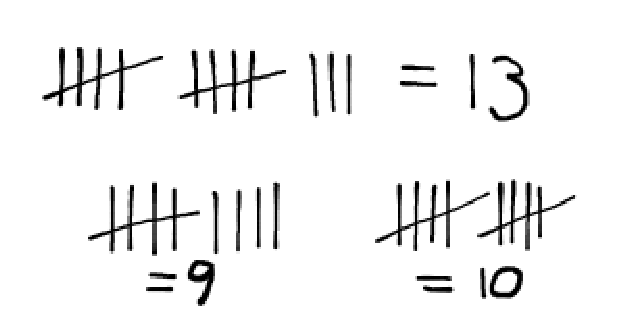
\includegraphics[width=4cm]{figs/strecktal.eps}
  \caption{%
    Tecknen i ett enkelt teckenvärdessystem.
  }\label{fig:Strecktal}
\end{figure}

Det romerska systemet är en modifiering av detta system.
Tecknen och deras betydelse i det romerska talsystemet ges i
\cref{tbl:RomerskaSiffror}.

\begin{table}
  \caption{%
    De romerska siffrorna.
  }\label{tbl:RomerskaSiffror}
  \begin{tabular}{ccccccc}
    \toprule
    I & V & X & L & C & D & M \\
    1 & 5 & 10 & 50 & 100 & 500 & 1000 \\
    \bottomrule
  \end{tabular}
\end{table}

Det romerska talsystemt fungerar nästan på samma sätt som ett
tecken\-värdes\-system.
Den väsentliga skillnaden är att i teckenvärdessystemet summeras alla tecknens
värden medan det i det romerska systemet även finns subtraktion.
I det romerska systemet subtraheras ett tecken av lägre värde som står före ett
tecken med högre värde.
Exempelvis, IV ger \(4\) eftersom att en etta står före en femma.
VI ger däremot \(6\) eftersom att tecknens värde summeras.
Talen 1-10 ges i \cref{tbl:RomerskaTal} och några andra större tal finns i
\cref{tbl:RomerskaTal2}.

\begin{table}
  \caption{%
    Talen 1-10 i det decimala och det romerska talsystemen.
  }\label{tbl:RomerskaTal}
  \begin{tabular}{lllllllllll}
    \toprule
    Decimala talsystemet & 1 & 2 & 3 & 4 & 5 & 6 & 7 & 8 & 9 & 10 \\
    Romerska talsystemt & I & II & III & IV & V &
      VI & VII & VIII & IX & X \\
    \bottomrule
  \end{tabular}
\end{table}

\begin{table}
  \caption{%
    Några tal skrivna med det romerska talsystemet.
  }\label{tbl:RomerskaTal2}
  \begin{tabular}{lll}
    \toprule
    \(2011\) & MMXI & \(1000+1000+10+1\) \\
    \(1999\) & MCMXCIX & \(1000+(1000-100)+(100-10)+(10-1)\) \\
    \(1998\) & MCMXCVIII & \(1000+(1000-100)+(100-10)+5+1+1+1\) \\
    \(587\) & DLXXXVII & \(500+50+10+10+10+5+1+1\) \\
    \(487\) & CDLXXXVII & \((500-100)+50+10+10+10+5+1+1\) \\
    \bottomrule
  \end{tabular}
\end{table}

Som kan ses i \cref{tbl:RomerskaTal2} är det eftersträvansvärt att så få
tecken som möjligt används vid subtraktion.
Exempelvis kan tänkas att \(487\) är \(500\) minus \(13\) och därför skulle
kunna skrivas som XIIID.\@
Det blir dock enklare att se om man istället använder C, eller \(100\), för
subtraktionen av D, eller \(500\), och sedan lägger till tecknen för \(87\)
som vanligt.

\begin{exercise}\label{xrc:RaknaMedRomerskaTal}
  Undersök och diskutera hur enkelt det är att räkna med och
  representera tal med det romerska talsystemet.
\end{exercise}
\begin{exercise}
  Med utgångspunkt i föregående övning, hur tror du att romarna bidragit till
  matematikhistorien?
\end{exercise}
\begin{exercise}
  Hur är det med talet noll och negativa tal i det romerska talsystemet?
\end{exercise}



%%%%%%%%%%%%%%%%%%%%%%%%%%%%%%%%%%%%%%%%%
% POSITIONSSYSTEM
%%%%%%%%%%%%%%%%%%%%%%%%%%%%%%%%%%%%%%%%%
\section{Positionssystem}%
\index{positionssystem}\index{talsystem!positionssystem}%
\label{sec:Positionssystem}
Som nämnts tidigare innebär ett positionssystem att samma tecken
har olika betydelse eller värde beroende på vilken position tecknet innehar.
Systemet har en \emph{talbas}.
Det decimala talsystemet har basen \(10\) och varje position motsvarar en
unik \(10\)-potens.
Siffran på denna position ger koefficienten för denna potens.

\begin{example}\label{ex:DecimaltPosistionssystem}
  Det decimala talsystemet har basen \(10\).
  Talet etthundratjugotre representeras i detta system som \(123\).
  Vi har då
  \[1\cdot10^2 + 2\cdot10^1 + 3\cdot10^0 = 100 + 20 + 3 = 123.\]
\end{example}
\begin{example}\label{ex:BinartPositionssystem}
  Det binära talsystemet har basen \(2\).
  Således representeras talet etthundratjugotre som \(1111011\).
  Vi har då
  \[1\cdot2^6 + 1\cdot2^5 + 1\cdot 2^4 + 1\cdot2^3 + 0\cdot2^2 +
  1\cdot2^1 + 1\cdot2^0 = 123.\]
\end{example}
\begin{example}
  Om ett positionssystem har basen \(b\) används då \(b\) antal siffror,
  dessa har värdena \(0, 1, 2, \ldots, b-1\).
  För att representera ett tal används summor av \(b\)-potenser där siffrans
  position avgör exponenten.
  Siffrans värde avgör koefficienten för, det vill säga hur många av, den
  specifika \(b\)-potensen som ska adderas.
  Det vill säga talet vars värde beräknas som
  \[
    d_1 b^{n-1} + d_2 b^{n-1} + \cdots + d_{n-1} b^1 + d_n b^0
  \]
  representeras som \(d_1d_2\cdots d_n\) i basen \(b\).
\end{example}

Det finns även andra talsystem, exempelvis babyloniernas
sexagesimala positionssystem%
\index{talsystem!babylonskt}\index{talsystem!sexagesimalt}
som hade basen \(60\).
Spår av detta kan vi idag se i hur vi räknar tid, att en minut har 60
sekunder och en timme har 60 minuter.
Vi använder dock inte 60 olika tecken för att representera våra sekunder och
minuter utan tar istället hjälp av det decimala talsystemet.
Det babylonska sexagesimalsystemet är det äldsta kända användandet av ett
positionssystem och härstammar från Babylonien\footnote{Babylonien låg i
södra delen av Mesopotamien, ungefär i dagens Irak.} omkring 3100 
f.v.t.~\cite{Kline1990mtf1}.

Kan då alla naturliga tal verkligen representeras med en godtycklig bas på
detta sätt?
Följande sats visar att sådant är fallet.
\begin{theorem}\label{thm:PositionssystemAllaUnika}
  Låt \(b>1\) vara ett naturligt tal större än ett.
  För varje naturligt tal \(x\in\N\) existerar ett naturligt tal \(n>0\)
  strikt större än noll och naturliga tal \(d_i<b\), där \(1\leq i\leq n\),
  strikt mindre än \(b\) sådana att \(x\) kan skrivas som
  \begin{equation*}
    x = d_1 b^{n-1} + d_2 b^{n-2} + \cdots + d_{n-1} b^1 + d_n b^0.
  \end{equation*}
  Denna presentation är unik upp till ordningen av termerna.
\end{theorem}
För att kunna bevisa detta behöver vi först följande lemma.
\begin{lemma}\label{lem:NollEndastOmLika}
  Låt \(b>0\) vara ett naturligt tal större än noll, \(m\) och \(n\)
  naturliga tal och \(c=c_1b^{n-1}+c_2b^{n-2}+\cdots+c_{n-1}b+c_n\), där
  \(0<c_1<b\) och \(0\leq c_i<b\) för \(i=2,3,\ldots,n\), och
  \(d=d_1b^{m-1}+d_2b^{m-2}+\cdots+d_{m-1}b+d_m\), där \(0<d_1<b\) och \(0\leq
  d_j<b\) för \(j=2,3,\ldots,m\).
  Då gäller att \(c-d=0\) endast om \(n=m\) och \(c_i=d_i\) för
  \(i=1,2,3,\ldots,n\).
\end{lemma}
\begin{proof}
  Låt oss anta att \(n=m+k\) för något naturligt tal \(k\).
  Vi har då att
  \begin{equation*}
    c-d=c_1b^{n-1}+\cdots+c_{k-1}b^{n-k+1}+(c_k-d_0)b^m+\cdots+(c_n-d_m) =
    0.
  \end{equation*}
  Men \(c_1b^{n-1}\neq 0\) och då måste \(n=m\).

  Då har vi att
  \begin{equation*}
    c-d = (c_1-d_1)b^{n-1}+\cdots+(c_{n-1}-d_{n-1})b+(c_n-d_n) = 0.
  \end{equation*}
  Låt oss anta att \(c_n-d_n\neq 0\), om inte delar vi med \(b\) tills att vi
  får en nollskild term utan en faktor \(b\).
  Då får vi att
  \begin{equation}
    \label{eq:NollEndastOmLika}
    (c_0-d_0)b^n+\cdots+(c_{n-1}-d_{n-1})b = -(c_n-d_n).
  \end{equation}
  Eftersom att vänsterledet i \cref{eq:NollEndastOmLika} är delbart med
  \(b\) måste även högerledet vara detta eftersom att de är lika.
  Men eftersom att \(c_i<b\) och \(d_i<b\) har vi att
  \(-b<c_i-d_i<b\) för \(i=0,1,2,\ldots,n\).
  Då är \(-(c_n-d_n)\) delbar med \(b\) endast om \(-(c_n-d_n)=0\), vilket
  är en motsägelse.
  Då måste alla termer \(c_i-d_i=0\) för \(i=1,2,3,\ldots,n\).
\end{proof}

Nu är vi redo att visa satsen.
\begin{proof}[Bevis \cref{thm:PositionssystemAllaUnika}]
  Vi börjar med att visa att summan existerar.
  Om vi delar \(x\) med \(b\) får vi en kvot \(q_1\) och en restterm
  \(r_1\) sådana att \(x=q_1b+r_1\) och \(0\leq r_1<b\).
  Om vi på samma vis delar \(q_1\) med \(b\) får vi en kvot \(q_2\) och en
  restterm \(r_2\) sådana att \(q_1=q_2b+r_2\) och \(0\leq r_2 < b\).
  Upprepas detta förfarande får vi att \(q_i=q_{i+1}b+r_{i+1}\), \(i\in\N\).
  Från \cref{xrc:KvotenMindre} har vi att \(q_{i+1}<q_i\) eftersom att
  \(b>1\).
  Vi får då från välordningsprincipen för de naturliga talen att \(q_n=0\)
  för något \(n\in\N\).
  Vi nu sätter ihop dessa resultat enligt följande idé.
  Vi hade först att \(x=q_1b+r_1\), men \(q_1=q_2b+r_2\) och följaktligen är
  \[x=(q_2b+r_2)b+r_1.\]
  Eftersom att \(q_i=q_{i+1}b+r_{i+1}\) får vi att
  \begin{align*}
    x &= ((((q_n b + r_n) b + r_{n-1}) b + \cdots + r_3) b + r_2) b + r_1 \\
     &= r_n b^{n-1} + r_{n-1} b^{n-2} + \cdots + r_3 b^2 + r_2 b^1 + r_1 b^0.
  \end{align*}
  Om vi låter \(d_1=r_n, d_2=r_{n-1}, \ldots, d_{n-1}=r_2, d_n=r_1\) ser vi
  att vi får en summa på korrekt form.

  Antag att det för ett naturligt tal \(x\) finns två olika representationer
  \(c_1c_2\cdots c_n\) och \(d_1d_2\cdots d_m\), båda med basen \(b\).
  Detta innebär att
  \begin{equation*}
    c_1 b^{n-1} + c_2 b^{n-2} + \cdots + c_n b^0 =
    x =
    d_1 b^{m-1} + d_2 b^{m-2} + \cdots + d_m b^0.
  \end{equation*}
  Då måste
  \begin{equation*}
    c_1b^{n-1}+c_2b^{n-2}+\cdots+c_n - d_1b^{m-1}+d_2b^{m-2}+\cdots+d_m =
    0,
  \end{equation*}
  men enligt \cref{lem:NollEndastOmLika} kan detta ej vara sant och vi har
  en motsägelse.
  Då måste det vara samma representation.
\end{proof}

\begin{exercise}
  Diskutera innebörden av denna sats och dess bevis.
\end{exercise}

\begin{example}
  Det kan nu vara av intresse med ett exempel där representationen ej är unik.
  Ett tydligt exempel är det romerska talsystemet där \(99\) skulle kunna
  representeras av både IC och XCIX.\@
  Representationen för tal i det romerska systemet är därmed inte unik.
\end{example}

Eftersom att vi enligt \cref{thm:PositionssystemAllaUnika} kan representera
alla naturliga tal i en godtycklig bas \(b>1\) större än ett och att denna
representation är unik kan vi med säkerhet definiera ett positionssystem enligt
följande.
\begin{definition}[Positionssystem]\index{talsystem!positionssystem}\index{positionssystem}\index{talbas}\index{positionssystem!talbas}\index{positionsvärdesystem|see{positionssystem}}\label{def:Positionssystem}
  Ett \emph{positionssystem}\footnote{%
    \emph{Eng.} positional system, place-value system
  }, eller positionsvärdesystem, har en
  \emph{talbas} \(b \in \N \setminus \{0,1\}\),
  siffrorna \(S=\{s\in\N\colon s<b\}\) och representerar ett tal \(x\in\N\) som
  \(d_1d_2\cdots d_n\), där \(d_i \in S\) är siffran på position \(i\), och
  \begin{equation}
    \nonumber
    x = d_1 b^{n-1} + d_2 b^{n-2} + \cdots + d_{n-1} b^1 + d_n b^0.
  \end{equation}
\end{definition}

\begin{example}\label{ex:DecimalaTalsystemet}
  Det decimala talsystemet har basen \(b=10\) och använder siffrorna
  \(S=\{0,1,2,3,4,5,6,7,8,9\}\).
\end{example}
\begin{example}\label{ex:BinaraTalsystemet}
  Det binära talsystemet har basen \(b=2\) och använder siffrorna
  \(S=\{0,1\}\).
\end{example}
\begin{example}\label{ex:HexadecimalaTalsystemet}
  Det hexadecimala talsystemet har basen \(b=16\).
  När ett talsystem har basen \(b>10\) används vanligtvis bokstäver från
  alfabetet som siffror för värdena \(10\), \(11\) och så vidare.
  Det hexadecimala talsystemet använder vanligtvis
  siffrorna \[S=\{0,1,2,3,4,5,6,7,8,9,A,B,C,D,E,F\},\] där \(A=10\),
  \(B=11\), \dots, \(F=15\).
\end{example}

För att kunna urskilja vilken talbas ett tal representeras med brukar basen
anges som ett subskript.
Exempelvis talet \(123\) skrivet med det decimala systemet anges som
\(123_{10}\).
Det blir då lättare att förstå \(123_{10} = 1111011_2\) som betyder att \(123\)
i bas 10 skrivs som \(1111011\) i bas 2.
Vanligtvis, när basen är självklar, brukar den utelämnas.
I de första 9 åren i grundskolan är det uteslutande det decimala talsystemet
som används och det har därför aldrig varit nödvändigt att där specificera att
basen varit 10.

\begin{exercise}\label{xrc:GiltigaTalbaser}
  Enligt \cref{def:Positionssystem} används inte talen \(0\) och \(1\)
  som baser, försök att förklara varför.
\end{exercise}
\begin{exercise}\label{xrc:RationelltPositionssystem}
  Vidareutveckla \cref{def:Positionssystem} till att även
  omfatta rationella tal.
\end{exercise}
\begin{exercise}\label{xrc:KomplettRationelltPositionssystem}
  Visa att alla rationella tal kan representeras med en godtycklig bas
  \(1<b\in\N\) enligt den nya definitionen från
  \cref{xrc:RationelltPositionssystem}.
\end{exercise}
\begin{exercise}\label{xrc:Decimalfoljder}
  Det rationella talet \(\frac{1}{3} = 0.333\ldots\) skrivs som en oändlig
  decimalutveckling i bas \(10\).
  Är det så i alla baser \(1<b\in\N\)?
\end{exercise}
\begin{exercise}\label{xrc:Basbyte}
  Försök att formulera en metod för att byta talbas för ett tal.
\end{exercise}


%%%%%%%%%%%%%%%%%%%%%%%%%%%%%%%%%%%%%%%%%%%%%%%%%%%%%%%%%%%%%%
% BYTE AV TALBAS
%%%%%%%%%%%%%%%%%%%%%%%%%%%%%%%%%%%%%%%%%%%%%%%%%%%%%%%%%%%%%%
\section{Byte av talbas}
Eftersom att \cref{thm:PositionssystemAllaUnika} säger att alla
naturliga tal kan representeras i alla baser innebär detta att samma tal har
en unik representation i varje bas.
Det kan då vara intressant att se ett tals olika representationer i olika
baser.
Hur detta basbyte går till och att det fungerar framgår av beviset för satsen.
Metoden illustreras här med nedan givna exempel.
\begin{example}
  Talet \(123_{10} = 1111011_2\), detta finner vi genom följande:
  \begin{align*}
    123 &= 61\cdot 2 + 1 \\
    61 &= 30\cdot 2 + 1 \\
    30 &= 15\cdot 2 + 0 \\
    15 &= 7\cdot 2 + 1 \\
    7 &= 3\cdot 2 + 1 \\
    3 &= 1\cdot 2 + 1 \\
    1 &= 0\cdot 2 + 1
  \end{align*}
  Då får vi
  \begin{multline}
%    (((((((0+1)\cdot2 + 1)\cdot2 + 1)\cdot2 + 1)\cdot2 + 1) + 0)\cdot2 + 1)
%      \cdot2 + 1 \\
    1 + 2\cdot (1 + 2\cdot (0 + 2\cdot (1 + 2\cdot (1 + 2\cdot (1 + 2\cdot
      (1 + 0)))))) \\
    = 1\cdot 2^6 + 1\cdot 2^5 + 1\cdot 2^4 + 1\cdot^3 + 0\cdot 2^2 +
      1\cdot 2^1 + 1\cdot 2^0 \\
    = 1111011_2 = 123_{10}.
  \end{multline}
\end{example}
\begin{example}
  Talet \(123_{10} = 7B_{16}\), detta finner vi genom följande:
  \begin{align*}
    123 &= 7\cdot16 + 11 \\
    7 &= 0\cdot16 + 7
  \end{align*}
  Således får vi siffrorna \(7\) och \(B\) samt att
  \begin{equation*}
    (0+7)\cdot16 + 11 = 7\cdot16^1 + 11\cdot16^0 = 7B_{16} = 123_{10}.
  \end{equation*}
  Detta betyder att \(7B_{16} = 123_{10}\) och därför är \(7B\) hexadecimalt
  samma tal som 123 är decimalt.
\end{example}

\begin{exercise}
  Vilket tal representerar \(123\) när det hexadecimala talsystemet används?
  Det vill säga, hur representeras \(123_{16}\) med basen 10?
\end{exercise}

\begin{exercise}\label{xrc:TalbasDatavetenskap}
  Inom datateknik är baserna \(2=2^1\), \(8=2^3\) och \(16=2^4\) väldigt
  populära, men bas \(10=2\cdot5\) är däremot inte lika populär.
  Datorns interna representation av tal sker i form av \emph{bitar} som kan
  anta värdena \emph{på} och \emph{av}, eller \(1\) och \(0\).
  Detta motsvarar precis det binära talsystemet, det vill säga basen
  \(2=2^1\), detta förklarar basens popularitet.
  Försök att förklara varför baserna \(8=2^3\) och \(16=2^4\) är populära,
  medan bas \(10=2\cdot5\) inte är det.
\end{exercise}



%%%%%%%%%%%%%%%%%%%%%%%%%%%%%%%%%%%%%%%%%%%%%%%%%%%%%%%%%%%%%%
% EN ADDITIONSALGORITM
%%%%%%%%%%%%%%%%%%%%%%%%%%%%%%%%%%%%%%%%%%%%%%%%%%%%%%%%%%%%%%
\section{En additionsalgoritm}
Positionens betydelse för siffrornas värde i positionssystemet gör
att tal representerade i detta talsystem blir väldigt enkla att räkna med.
Vi ska i detta avsnitt undersöka varför.

Vi inleder först med en illustration av algoritmen genom följande exempel.
\begin{example}
  Vi vill addera talen \(123_{10}\) och \(253_{10}\) i basen \(10\).
  Vi skriver dem då ovanför varandra och får då steg \verb'a)' nedan.
  \begin{verbatim}
     a)   1 2 3   b)   1 2 3  c)   1 2 3  d)   1 2 3
        + 2 5 3      + 2 5 3     + 2 5 3     + 2 5 3
        -------      -------     -------     -------
                           6         7 6       3 7 6
  \end{verbatim}
  Vi fortsätter genom att addera siffrorna i den sista kolumnen, det vill
  säga entalen.
  Vi får då \(3\) och \(3\), och totalt har vi \(6\).
  Detta tal skriver vi under raden och hamnar då i steg \verb'b)'.
  Vi fortsätter på samma sätt i stegen \verb'c)' och \verb'd)'.
  I steg \verb'c)' adderar vi tiotalen och i steg \verb'd)' adderar vi
  hundratalen.
  Summan av de två talen är talet som står under raden, det vill säga
  \(123+253=376\).
\end{example}
\begin{example}\label{ex:AdderaMedRest}
  Vi vill nu addera talen \(123_{10}\) och \(999_{10}\), fortfarande i basen
  \(10\).
  Vi gör då som ovan och får steg \verb'a)' nedan.
  \begin{verbatim}
                         1         1 1       1 1 1       1 1 1
     a)   1 2 3   b)   1 2 3  c)   1 2 3  d)   1 2 3  e)   1 2 3
        + 9 9 9      + 9 9 9     + 9 9 9     + 9 9 9     + 9 9 9
        -------      -------     -------     -------     -------
                           2         2 2       1 2 2     1 1 2 2
  \end{verbatim}
  Vi fortsätter genom att addera siffrorna i den sista kolumnen, det vill
  säga entalen \(3\) och \(9\), och får då \(12\).
  Eftersom att vi får \(12\) ental innebär detta att vi får ett tiotal och
  två ental.
  Tiotal adderas tillsammans med tiotal och vi skriver \(1\) ovanför kolumnen
  med tiotal.
  Vi hamnar då i steg \verb'b)'.
  I steg \verb'c)' adderar vi kolumnen med talen \(1, 2\) och \(9\), det vill
  säga alla tiotal.
  Vi får åter \(12\) och gör som i steg \verb'b)' eftersom att \(12\) tiotal
  innebär att vi har ett hundratal och två tiotal.
  I steg \verb'c)' när vi adderar \(1,1\) och \(9\) får vi \(11\).
  Detta innebär att vi får ett hundratal och ett tusental.
  Eftersom att det inte fanns några tusental i de båda termerna skriver vi
  tusentalet ovanför den tomma kolumnen till vänster, detta visas i steg
  \verb'd)'.
  I steg \verb'e)' adderar vi \(1,0\) och \(0\) och får \(1\) som skrivs
  under raden.
  Då får vi att \(123+999=1122\).
\end{example}
\begin{remark}
  Notera att tiotalet ges av kvoten vid heltalsdivision med basen som
  nämnare, dessutom ges entalet av resten vid denna heltalsdivision.
%  Notera att entalet ges av resten vid heltalsdivision med basen som nämnare
%  och tiotalet ges av heltalskvoten. %vid denna heltalsdivision.
\end{remark}

Vi vill nu titta på det generella fallet med en godtycklig bas \(b>1\).
När vi ovan adderar kolumnerna kan vi få ett en- eller tvåsiffrigt tal som
resultat.
Till exempel när vi i \cref{ex:AdderaMedRest} steg \verb'b)' adderar \(3\)
och \(9\) får vi det tvåsiffriga talet \(12\).
Om \(b>1\) är basen i ett talsystem, \(s<b\) och \(t<b\) är två siffror i detta
talsystem.
Då är summan \(0\leq s+t\leq 2(b-1)\).
Om summan \(s+t\) är strikt mindre än \(b\) följer det av
\cref{thm:PositionssystemAllaUnika} att summan är ensiffrig.
Följande lemma fastställer att om summan \(s+t\) är större än \(b\) och mindre
än \(2(b-1)\) då är summan exakt tvåsiffrig.
\begin{lemma}\label{lem:AdditionSiffror}
  Ett naturligt tal \(x\) i intervallet \(b \leq x \leq 2(b-1)\) kan skrivas
  som en summa \(x = d_1b^1 + d_2b^0\),
  där \(1 \leq d_1 \leq b-1\) och \(0 \leq d_2 \leq b-1\).
\end{lemma}
\begin{proof}
  Det är klart från \cref{thm:PositionssystemAllaUnika} att \(x\) kan
  skrivas som en summa på formen \(d_1 b^{n-1} + \cdots + d_n b^0\) och att 
  denna är unik.
  Det som återstår att visa är att den består av enbart två termer, det vill
  säga att \(n=2\).

  Om vi tittar på fallet \(x=b\) får vi vid heltalsdivision kvoten \(x/b = 1\)
  och resttermen \(0\).
  Det vill säga, vi har \(d_1=1\), \(d_2=0\) och således \(x=1\cdot b+0\).
  Då måste vi ha minst två termer.

  Om vi tittar på fallet \(x=2(b-1)\) ser vi att \(2(b-1)=b+(b-2)\).
  Heltalsdivisionen \(x/b\) ger då kvoten \(b/b=1\) och resttermen \(b-2\).
  Vi har således \(d_1=1\), \(d_2=b-2\) och följaktligen
  \(x=1\cdot b+(b-2)\).

  Då har vi exakt två termer.
\end{proof}

\begin{exercise}
  Diskutera innebörden av detta lemma och dess bevis.
\end{exercise}

Innan vi går vidare till satsen som visar att denna additionsmetod fungerar
måste vi ha lite notation för att underlätta formuleringarna.
Låt \(q_b\) vara en funktion sådan att den ger kvoten vid heltalsdivisionen
\(t/b\) och beteckna denna som \(q_b(t)\).
Låt också \(r_b\) vara en funktion sådan att den ger resten vid
heltalsdivisionen \(t/b\) och beteckna denna som \(r_b(t)\).
Då har vi att \(t=q_b(t)\cdot b+r_b(t)\).
\begin{example}
  Vi har att \(q_5(7)=7/5=1\) och \(r_5(7)=7-q_5(7)\cdot 5=2\).
\end{example}
\begin{example}
  Vi har att \(q_{10}(7)=7/10=0\) och \(r_{10}(7)=7-q_{10}(7)\cdot 10=7\).
\end{example}

Följande sats visar att denna additionsmetod fungerar för godtyckligt långa tal
\(x=x_1x_2\cdots x_n\) och \(y=y_1y_2\cdots y_m\) representerade i samma talbas
\(b>1\).
\begin{theorem}[Additionsalgoritm]
  Låt \(x=x_1x_2\cdots x_n\) och \(y=y_1y_2\cdots y_m\) vara två tal
  representerade i ett positionssystem med basen \(b>1\),
  \(x_i\) och \(y_i\) vara identiskt noll för \(i<1\) och \(N=\max\{n,m\}\).
  Låt också \(q_b(t)=t/b\) vara kvoten och \(r_b(t)\) vara resten vid
  heltalsdivisionen \(t/b\).
  Summan \(x+y\) kan då fås genom 
  \begin{multline}\label{eq:AdditionsEkvation}
    x+y= q_b(x_{n-N}+y_{m-N})b^N + \\
    \left(r_b(x_{n-N}+y_{m-N})+q_b(x_{n-N+1}+y_{m-N+1})\right)b^{N-1} +\\
    \left(r_b(x_{n-N+1}+y_{m-N+1})+q_b(x_{n-N+2}+y_{m-N+2})\right)b^{N-2}
      + \\
    \cdots + \left(r_b(x_{n-1}+y_{m-1})+q_b(x_n+y_m)\right)b^1 +
    r_b(x_n+y_{m})b^0.
  \end{multline}
\end{theorem}
\begin{proof}
  Låt oss först antaga att \(n=m+k\).
  Om vi tittar på \(x=x_1 b^{n-1} + x_2 b^{n-2} + \cdots + x_n b^0\) och
  \(y = y_1 b^{m-1} + y_2 b^{m-2} + \cdots + y_m b^0\) får vi att
  \begin{align*}
    x+y=&x_1b^{n-1}+\cdots+x_{k-1}b^{n-k+1}+(x_k+y_1)b^m+\\
    &(x_{k+1}+y_2)b^{m-1}+\cdots+(x_{n-1}+y_{m-1})b^1+(x_n+y_m)b^0
  \end{align*}
  Vi fortsätter med att titta på en av termerna \((x_{i+k}+y_i)b^{n-k-i}\)
  och vi ser att \(0\leq x_{i+k}+y_i\leq b-2\).
  Vi har från \cref{lem:AdditionSiffror} att om \(b\leq x_{i+k}+y_i\leq
  2(b-1)\) är \(x_{i+k}+y_i = d_1b+d_2\) med \(1\leq d_1<b\) och \(0\leq
  d_2<b\) och \(x_{i+k}+y_i = d < b\) annars.

  Vi tittar på det första fallet.
  Vi får då att
  \begin{align*}
    (x_{i+k}+y_i)b^{n-k-i} &= (d_1b+d_2)b^{n-k-i}
      = d_1b^{n-k-i+1}+d_2b^{n-k-i}.
  \end{align*}
  Vi har att \(q_b(d_1b+d_2)=d_1\) och att \(r_b(d_1b+d_2)=d_2\) och således
  att
  \begin{equation*}
    (x_{i+k}+y_i)b^{n-k-i} = q_b(x_{i+k}+y_i)b^{n-k-i+1} +
    r_b(x_{i+k}+y_i)b^{n-k-i}.
  \end{equation*}
  Om \(x_{i+k}+y_i<b\) har vi att \(q_b(x_{i+k}+y_i)=0\) och
  \(r_b(x_{i+k}+y_i)=x_{i+k}+y_i\), då får vi även med det andra fallet.

  Vi ser i \cref{eq:AdditionsEkvation} att båda dessa termer finns med.
  \(q_b(x_{i+k}+y_i)\) finns med som en del i \(b^{n-k-i+1}\)-potensen och
  \(r_b(x_{i+k}+y_i)\) finns med som en del i \(b^{n-k-i}\)-potensen.

  Vi kan således konstatera att likheten i \cref{eq:AdditionsEkvation} är
  korrekt.
\end{proof}
\begin{exercise}
  Diskutera innebörden av denna sats och dess bevis.
\end{exercise}

Med detta har vi visat att additionsmetoden fungerar för en godtycklig bas
\(b>1\) i ett positionssystem.
Alla \(q_b\)-termerna motsvarar tiotalet som skrivs ovanför vänstervarande
kolumn om summan blir för stor.
Om summan inte blir för stor blir \(q_b\)-termen noll.
Alla \(r_b\)-termerna motsvarar entalet som alltid skrivs under strecket.

\begin{exercise}\label{xrc:MultiplikationsAlgoritm}
  Undersök om den välkända multiplikationsalgoritmen, som elever lär sig i den
  svenska grundskolan, även den fungerar för alla baser \(1<b\in\N\).
\end{exercise}


\ifdraft{}{%
  \part{Ekvationer}
}
\chapter{Ekvationer}
\label{ch:Ekvationer}
\dots

\chapter{Olikheter}
\label{ch:Olikheter}
\dots

\chapter{Potensekvationer}
\label{ch:Potensekvationer}
\dots

\ifdraft{}{%
  \part{Geometri}
}
\chapter{Klassisk geometri}
\label{ch:Geometri}
\dots

\chapter{Trigonometri}
\label{ch:Trigonometri}
\dots

\chapter{Linjär algebra}
\label{ch:LinjarAlgebra}
\dots

\ifdraft{}{%
  \part{Samband och förändring}
}
\chapter{Procent och andra relativa storheter}
\label{ch:Procent}
\dots

\chapter{Olika former av förändring}
\label{ch:Forandring}
\dots

\ifdraft{}{%
  \part{Kombinatorik, sannolikhet och statistik}
}
% Copyright 2013, 2014, 2015, 2016; Daniel Bosk <daniel@bosk.se>
%
% This work is licensed under the Creative Commons Attribution-ShareAlike 4.0 
% Unported license.  To view a copy of this license, visit URL
%
%   http://creativecommons.org/licenses/by-sa/4.0/.
%

\chapter{Grundläggande kombinatorik}
\label{GrundläggandeKombinatorik}
% XXX Skriv kapitlet om kombinatorik
\lettrine{K}{ombinatorik handlar} om studiet av diskreta strukturer.
Den gren av kombinatoriken som vi ska behandla i detta kapitel är 
\emph{uppräknelig kombinatorik}.
\index{kombinatorik}
\dots

\begin{lemma}[Additionsprincipen]
\label{Additionsprincipen}
\index{additionsprincipen}
  Låt \(u_1, \dots, u_n\) vara \(n\) disjunkta mängder.
  Då är kardinaliteten \(|u_1\cup \cdots\cup u_n| = |u_1| + \cdots + |u_n|\).
\end{lemma}
\begin{proof}
  \dots
\end{proof}

\begin{lemma}[Multiplikationsprincipen]
\label{Multiplikationsprincipen}
\index{multiplikationsprincipen}
  Låt \(u_1, \dots, u_n\) vara \(n\) mängder.
  Då är kardinaliteten \(|u_1\times \cdots\times u_n| = |u_1|\cdots |u_n|\).
\end{lemma}
\begin{proof}
  \dots
\end{proof}

\begin{definition}[Permutation]
\label{Permutation}
\index{permutation}
  \dots
\end{definition}

\begin{theorem}[Antalet permutationer]
\label{AntaletPermutationer}
  \dots
\end{theorem}
\begin{proof}
  \dots
\end{proof}

\begin{definition}[Kombination]
\label{Kombination}
\index{kombination}
  \dots
\end{definition}

\begin{theorem}[Antalet kombinationer]
\label{AntaletKombinationer}
  \dots
\end{theorem}
\begin{proof}
  \dots
\end{proof}

\begin{theorem}[Dirichlets lådprincip\footnote{Även 
    duvhålsprincipen}]
\label{thm:ladprincipen}
\index{Dirichlets lådprincip}
\index{lådprincipen}
\index{duvhålsprincipen}
  % XXX Beskriv Dirichlets lådprincip
  \dots
\end{theorem}
\begin{proof}
  \dots
\end{proof}


\section{Om val}
Vi stöter ofta på val av olika slag.
Vi ska i detta avsnitt reflektera över antalet möjliga utfall som kan uppstå
genom att olika val kombineras samman.

Vi inleder med definitioner av de begrepp vi kommer att använda.

\begin{definition}\label{def:Val}
  Med \emph{val} menas att det finns \(n \geq 1\) antal distinkta alternativ
  att välja mellan, av dessa alternativ måste ett och endast ett väljas.
  Det alternativ som väljs sägs vara \emph{utfallet av valet}.
\end{definition}

Vi fortsätter med ett väldigt enkelt lemma om förhållandet mellan valets
antal alternativ och det möjliga antalet utfall.

\begin{lemma}\label{lem:AntalUtfall}
  Ett val från \(n\) alternativ har \(n\) möjliga utfall.
\end{lemma}
\begin{proof}
  För varje alternativ behövs åtminstone ett utfall.
  Om vi har \(n\) alternativ och antar att vi har \(n+1\) utfall,
  då måste det enligt Dirichlets lådprincip, \cref{thm:ladprincipen}, vara 
  något alternativ som får fler än ett utfall.
  Men om ett och samma alternativ har flera utfall, då måste dessa utfall
  vara samma utfall.
  Detta är en motsägelse och därför måste vi ha exakt \(n\) utfall.
\end{proof}

För fullständighet inkluderas även följande exempel.
\begin{example}\label{ex:Fikabrod}
  Du ska välja fikabröd till eftermiddagsfikat.
  De alternativ du har att välja mellan är en nybakad bulle, en torr kaka och
  att inte ta något fikabröd.
  Notera att välja \emph{ingenting} utgör ett alternativ, det går alltså inte
  att avstå från ett val.

  Valet av fikabröd har tre alternativ, enligt \cref{lem:AntalUtfall}
  finns således tre möjliga utfall.
  Ett utfall är att vi väljer bullen, ett annat att vi väljer kakan och det
  sista att vi väljer att inte ta något fikabröd.
\end{example}

\subsection{Att välja bland val}
Då är det dags att utöka våra möjligheter att välja genom att kombinera flera
val till ett sammansatt val.

\begin{definition}
  När ett val ska göras följt efter ett annat säger vi att vi har ett
  \emph{sammansatt val}.
  Ett sammansatt val kan ibland kallas för val.
  Varje ingående val kallas för ett \emph{delval}.
\end{definition}

\begin{example}
  Det är dags för eftermiddagsfika igen.
  Du ska först välja om du ska dricka kaffe, te eller vatten.
  (Att inte välja någonting är inte ett alternativ i detta val, detta är ett
  rent teoretiskt val eftersom att rent praktiskt finns ju alltid
  alternativet att inte fika alls.)
  Därefter ska du välja fikabröd enligt \cref{ex:Fikabrod}.
  Då har vi ett sammansatt val bestående av två delval, ett för dryck och ett
  för fikabröd.
\end{example}
\begin{exercise}
  Visa att detta stämmer överens med att välja mellan alternativen \emph{kaffe 
  och bulle}, \emph{kaffe och kaka}, \emph{te och bulle}, och så vidare.
\end{exercise}

Det är nu intressant att veta hur många möjliga utfall som ett sådant val
möjligen kan ha.
Detta sammanfattas i följande sats.

\begin{theorem}[Multiplikationsprincipen]\label{thm:Multiplikationsprincipen}
  Ett sammansatt val av \(m\) antal delval, där delval \(i\) har \(n_i\)
  antal alternativ,
  har \(n_1\cdot n_2\cdots n_m\) antal möjliga utfall.
\end{theorem}

\begin{proof}
  Låt oss börja med att titta på det sista valet, val \(m\).
  Detta val har \(n_m\) alternativ och således \(n_m\) utfall enligt
  \cref{lem:AntalUtfall}.
  Vi går vidare till valet innan, det vill säga val \(m-1\).
  Detta val har \(n_{m-1}\) möjliga utfall.
  För varje utfall av detta val kan vi få \(n_m\) utfall i val \(m\).
  Då har vi alltså tillsammans
  \begin{equation}\label{eq:MultprincipTvaVal}
    \sum_{k=1}^{n_{m-1}} n_m = \underbrace{n_m + n_m + \cdots
    n_m}_{n_{m-1}} = n_{m-1}\cdot n_m.
  \end{equation}
  För varje utfall av delval \(m-2\) kan vi få antalet utfall från
  \cref{eq:MultprincipTvaVal}.
  Det vill säga
  \begin{equation}
    \sum_{k=1}^{n_{m-2}} n_{m-1}\cdot n_m = n_{m-2}\cdot n_{m-1} \cdot n_m.
  \end{equation}
  Vi fortsätter på detta vis till vi når det första valet då vi får
  \begin{equation}
    \sum_{k=1}^{n_1} n_2\cdot n_3\cdots n_{m-2}\cdot n_{m-1}\cdot n_m
      = n_1\cdot n_2\cdots n_m,
  \end{equation}
  vilket visar satsen.
\end{proof}

Från \cref{thm:Multiplikationsprincipen} följer direkt ett enkelt resultat
som vi ger i detta korollarium\footnote{%
  Det vill säga en följdsats.
}.

\begin{corollary}\label{cor:SammansattValKonstAlternativ}
  Ett sammansatt val av \(m\) antal delval där varje delval har \(n\)
  alternativ, har \(n^m\) antal möjliga utfall.
\end{corollary}

\begin{proof}
  Om vi har ett sammansatt val av \(m\) antal delval, där delval
  \(i\) har \(n_i\) alternativ.
  Då har vi enligt \cref{thm:Multiplikationsprincipen} att det totala
  utfallet är \(n_1\cdot n_2\cdots n_m\).
  Men eftersom att alla val hade samma antal alternativ, nämligen \(n\), då
  får vi att \(n_1\cdot n_2\cdots n_m = n\cdot n\cdots n = n^m\).
  Följaktligen får vi \(n^m\) antal möjliga utfall då vi har \(m\) delval där
  varje delval har \(n\) alternativ.
\end{proof}



\section{Val av lösenord}
Vi ska nu titta på hur detta kan användas för att undersöka säkerheten hos
lösenord.
Det finns flera angreppssätt för att skapa lösenord, exempelvis genom att
välja en kombination av tecken (bokstäver, siffror och specialtecken) eller att
helt enkelt välja några ord.
Det går också att skapa lösenord genom att slumpmässigt välja några ord som
kombineras till ett lösenord.

Vi börjar med det första fallet, där vi skapar ett lösenord genom att kombinera
tecken.
Om vi ska skapa ett lösenord som är fem tecken långt och får innehålla
bokstäverna A-Z, både gemener och versaler,
siffrorna 0-9 samt
specialtecknen ''!@.\%\&'',
då kan vi se valet av lösenord som ett sammansatt val bestående av fem delval,
där alternativen för varje delval är de tillåtna tecknen.
Antalet alternativ är således \(26\cdot 2 + 10 + 5 = 67\).
Eftersom att alla delval har samma antal alternativ kan vi använda
\cref{cor:SammansattValKonstAlternativ} för att ta reda på antalet möjliga
utfall, det vill säga antalet möjliga lösenord.
Antalet lösenord som uppfyller detta krav är \(67^5 = 1350125107\).

Nu fortsätter vi med att titta på fallet med att välja lösenord genom att
slumpmässigt välja några ord.
Vi bestämmer oss för att använda ett lösenord med fyra slumpmässigt valda
ord från svenska språket.
Enligt Svenska Akademin \citep{SAOL} innehåller Svenska Akademins Ordlista
ungefär 125000 ord.
Detta ger enligt \cref{cor:SammansattValKonstAlternativ}
\begin{equation}\label{eq:AntalUtfallOrd}
  125000^4 = (2^3\cdot 5^6)^4
    = 2^{12}\cdot 5^{24}
    = 2^{12}\cdot 25^{12},
\end{equation}
det vill säga \(244140625000000000000\), möjliga lösenord.

Det senaste fallet kan också ses ur det första fallets perspektiv.
Låt oss anta att medellängden av orden vi väljer från är fem tecken och att
dessa tecken enbart är gemener.
Det innebär att vi får
\begin{equation}\label{eq:AntalUtfallTecken}
  (29^5)^4 = 29^{20} = 176994576151109753197786640401
\end{equation}
möjliga lösenord.

Hur spelar denna representation någon roll, vad betyder skillnaden mellan
\cref{eq:AntalUtfallOrd} och \cref{eq:AntalUtfallTecken}?
Det första som bör påpekas är att i \cref{eq:AntalUtfallTecken} tas även
teckenkombinationer som ej är svenska ord med.
Detta eftersom att valet var att välja fyra uppsättningar av fem tecken.
Betydelsen av detta är att om vi låter en dator bara slumpa fram 20 bokstäver
(gemener), då kommer det att resultera i antalet gissningar från
\cref{eq:AntalUtfallTecken}.
Det är inte ens säkert att datorn kommer att hitta rätt lösenord om vi råkade
välja fyra långa ord som alla var minst sex bokstäver långa.
Detta är ett problem med denna uppskattning.
Om vi däremot har en ordlista som datorn väljer ord från för att kombinera
dessa till ett lösenord om fyra ord för att gissa lösenordet, då kommer antalet
gissningar att maximalt bli \cref{eq:AntalUtfallOrd}.
Även denna metod kräver naturligtvis att orden i lösenordet finns med i
ordlistan som datorn har tillgång till.


%\include{pwdanalysis/pwdinclude}
\chapter{Sannolikhetsteori}
\label{ch:Sannolikhet}
\dots

% Copyright 2017; Daniel Bosk <daniel@bosk.se>
%
% This work is licensed under the Creative Commons Attribution-ShareAlike 4.0 
% Unported license.  To view a copy of this license, visit URL
%
%   http://creativecommons.org/licenses/by-sa/4.0/.
%

\chapter{Sannolikhetsfördelningar}
\label{Sannolikhetsfordelningar}

\dots


\section{Bernoullifördelningen}

\dots


\section{Binomialfördelningen}

\dots


\section{Likformig sannolikhetsfördelning}

\dots


\section{Multinomialfördelningen}

\dots


\section{Hypergeometrisk fördelning}

\dots


\section{För-förstagångenfördelningen}

\dots


\section{Poissonbinomialfördelningen}

\dots


\section{Poissonfördelningen}

\dots


\section{Normalfördelningen}

\dots


\section{Laplacefördelningen}

\dots

\chapter{Statistikteori}
\label{ch:Statistik}
\dots

%\include{krypto/krypto}

% appendices
\appendix
\ifdraft{%
  \doublespacing{}
}{}
\chapter{Studiehandledning för Matematik 1c}\label{Studiehandledning}
%\nocite{Tobin2005msl}

\lettrine{K}{ursen Matematik 1c}
är enligt ämnesplanen 100 poäng, det vill säga att den ska ges 100 
lektionstimmar.
Dessa lektionstimmar ska fördelas på de fem huvudområden som ges under rubriken
\emph{Centralt innehåll} i ämnesplanen: 
\begin{itemize}
  \item taluppfattning, aritmetik och algebra;
  \item geometri;
  \item samband och förändring;
  \item sannolikhet och statistik; samt
  \item problemlösning.
\end{itemize}

I planeringen given nedan avser tidsåtgången lärargenomgångar, till exempel
tid när läraren går igenom innehåll vid tavlan.
Denna tid innefattar inte elevers egna arbete, redovisningar av uppgifter,
klassrumsdiskussioner etcetera.

Avsnittet \emph{Problemlösning}, som innehåller punkterna
\begin{itemize}
  \item Strategier för matematisk problemlösning inklusive användning av
    digitala medier och verktyg,
  \item Matematiska problem av betydelse för privatekonomi, samhällsliv och
    tillämpningar i andra ämnen, och
  \item Matematiska problem med anknytning till matematikens kulturhistoria,
\end{itemize}
kan med fördel inkluderas i undervisningen som tar upp övriga områden och
behöver således inte behandlas specifikt.

Inledande i kursen bör vara grundläggande logik\footnote{%
  Från området \emph{Geometri} har vi punkten \enquote{Matematisk argumentation 
    ned hjälp av grundläggande logik inklusive implikation och ekvivalens samt 
    jämförelser med hur man argumenterar i vardagliga sammanhang och inom 
    naturvetenskapliga ämnen}.
}, begreppen definition och axiom samt sats och bevis\footnote{%
  Från området \emph{Geometri} har vi punkten \enquote{Illustration av 
    begreppen definition, sats och bevis, till exempel med Pythagoras sats och 
    triangelns vinkelsumma}.
}.
Detta eftersom att dessa fundamentala begrepp är det som bygger upp
matematiken.
Därefter kan grundläggande mängdlära gås igenom, med axiom och grundläggande
satser, och konstruktionen av de naturliga talen kan visas för att visa hur
matematiken fundamentalt är uppbyggd.
För detaljer se \cref{tbl:inledning}.

\begin{table}
  \caption{%
    Planering för inledningen.
  }\label{tbl:inledning}
  \begin{tabular}{ll}
    Innehåll & Tidsåtgång (timmar) \\
    \toprule
    Logik, definition, sats och bevis. & 2 \\
    \midrule
    Mängder. & 1 \\
    \midrule
    Mängden av naturliga tal. & 1 \\
    \bottomrule
    & 4 \\
  \end{tabular}
\end{table}

Därefter följer lämpligen avsnittet \emph{Taluppfattning, aritmetik
och algebra} eftersom att taluppfattning, aritmetik och algebra är nödvändiga
för vidare studier av matematiken, och alltså nödvändiga för resten av kursen,
samt att det är naturligt att studera heltalen efter de naturliga talen.
För detaljer se \cref{tbl:talteori}.
%Eftersom att avsnittet har fem punkter bör \emph{25 timmar} avsättas för hela
%detta område.

\begin{table}
  \caption{%
    Planering för avsnittet \emph{Taluppfattning, aritmetik och
    algebra}.
  }\label{tbl:talteori}
  \begin{tabular}{ll}
    %\textbf{Innehåll} & \textbf{Tidsåtgång (timmar)} \\
    Innehåll & Tidsåtgång (timmar) \\
    \toprule
    Generalisering av aritmetikens räkneregler till att\\
      hantera algebraiska uttryck. & 2 \\
    \midrule
    Egenskaper hos mängden heltal, olika talbaser samt\\
      begreppen primtal och delbarhet. & 5 \\
    \midrule
    Egenskaper hos mängderna rationella tal, irrationella\\
      tal och reella tal. & 5 \\
    \midrule
    Begreppet linjär olikhet. & 1 \\
    \midrule
    Algebraiska och grafiska metoder för att lösa linjära\\
      ekvationer, olikheter och potensekvationer. & 5 \\
    \midrule
    Metoder för beräkningar inom vardagslivet och\\
      karaktärsämnena med reella tal skrivna på olika\\
      former, inklusive potenser med reella exponenter\\
      samt strategier för användning av digitala verktyg.
      & * \\
    \bottomrule
    & 21 \\
  \end{tabular}
\end{table}

Efter egenskaperna hos heltal, rationella och irrationella tal och algebra kan
funktionsbegreppet introduceras.
Funktionsbegreppet är ett centralt begrepp inom all matematik och bör gås
igenom tidigt i kursen för att kunna användas senare, exempelvis när
de trigonometriska funktionerna och logaritmfunktionen introduceras.
För detaljer se \cref{tbl:funktioner}.

\begin{table}
  \caption{%
    Planering för avsnittet \emph{Samband och förändring}.
  }\label{tbl:funktioner}
  \begin{tabular}{ll}
    Innehåll & Tidsåtgång (timmar) \\
    \toprule
    Begreppen funktion, definitions- och värdemängd samt\\
      egenskaper hos linjära funktioner samt potens-\\
      och exponentialfunktioner. Representationer av\\
      funktioner i form av ord, funktionsuttryck, tabeller\\
      och grafer.  & 6 \\
    \midrule
    Skillnader mellan begreppen ekvation, olikhet, algebraiskt\\
      uttryck och funktion. & 2 \\
    \midrule
    Fördjupning av procentbegreppet: promille, ppm och\\
      procentenheter. & 2 \\
    \midrule
    Begreppen förändringsfaktor och index samt metoder för\\
      beräkning av räntor och amorteringar för olika typer\\
      av lån. & 4 \\
    \bottomrule
    & 14 \\
  \end{tabular}
\end{table}

Då föregående avsnitt \emph{Samband och förändring} avslutas med
procentbegreppet är det lämpligt att fortsätta med detta i avsnittet
\emph{Sannolikhet och statistik}.
Procentbegreppet används då i en annan form än som ett mått av förändring och
eleverna får bygga vidare sin förståelse för hur procentbegreppet kan användas.
Sannolikhetsavsnittet är ett relativt till kursen litet avsnitt, för detaljer
se \cref{tbl:sannolikhet}.

\begin{table}
  \caption{%
    Planering för avsnittet \emph{Sannolikhet och statistik}.
  }\label{tbl:sannolikhet}
  \begin{tabular}{ll}
    Innehåll & Tidsåtgång (timmar) \\
    \toprule
    Begreppen beroende och oberoende händelser samt\\
      metoder för beräkning av sannolikheter vid slumpförsök\\
      i flera steg med exempel från spel och risk- och\\
      säkerhetsbedömningar. & 3 \\
    \midrule
    Granskning av hur statistiska metoder och resultat används\\
      i samhället och i vetenskap. & 3 \\
    \bottomrule
    & 6 \\
  \end{tabular}
\end{table}

Det sista avsnittet i kursen är avsnittet \emph{Geometri}.
Detta avsnitt är ett avskiljt område som har stor historisk betydelse för
matematiken.
I denna presentation kommer funktionsbegreppet att användas vid introduktionen
av de trigonometriska funktionerna, och därför bör geometriavsnittet följa
efter introduktionen av funktionsbegreppet.
För detaljer se \cref{tbl:geometri}.

\begin{table}
  \caption{%
    Planering för avsnittet \emph{Geometri}.
  }\label{tbl:geometri}
  \begin{tabular}{ll}
    Innehåll & Tidsåtgång (timmar) \\
    \toprule
    Pythagoras sats & 1 \\
    \midrule
    Begreppen sinus, cosinus och tangens samt metoder för\\
      beräkning av vinklar och längder i rätvinkliga\\
      trianglar. & 4 \\
    \midrule
    Begreppet vektor och dess representationer såsom riktad\\
      sträcka och punkt i ett koordinatsystem. & 1 \\
    \midrule
    Addition och subtraktion med vektorer, produkten av en\\
      skalär och en vektor samt skalärprodukt av vektorer\\
      i ett koordinatsystem. & 3 \\
    \midrule
    Pythagoras sats i \(N\) dimensioner. & 1 \\
    \bottomrule
    & 10 \\
  \end{tabular}
\end{table}

Avslutningsvis sammanfattas kursplaneringen översiktligt 
i \cref{tbl:sammanfattning}.
Totalt är 55 timmar avsatt för genomgångar, de återstående 45 timmarna är
oplanerade och bör användas till exempelvis elevers egna arbete, redovisning
av uppgifter, klassrumsdiskussioner etcetera.
Dessa timmar skulle kunna spridas jämnt över alla områden, men de bör hellre
nyttjas där eleverna har intresse eller behov av mer tid.

\begin{table}
  \caption{%
    Kursplaneringsöversikt.
  }\label{tbl:sammanfattning}
  \begin{tabular}{ll}
    Innehåll & Tidsåtgång (timmar) \\
    \toprule
    Inledning & 4 \\
    Taluppfattning, aritmetik och algebra & 21 \\
    Samband och förändring & 14 \\
    Sannolikhet och statistik & 6 \\
    Geometri & 10 \\
    \midrule
    & 55 \\
    \bottomrule
    Oplanerad tid & 45 \\
  \end{tabular}
\end{table}



\backmatter{}
\ifdraft{%
  \singlespacing{}
}{}
\printbibliography{}
\ifdraft{}{%
  \listoffigures
  \listoftables
}
%\printnomenclature
\printindex



\clearpage
\end{document}
